%% LaTeX2e class for student theses
%% thesis.tex
%% 
%% Karlsruhe Institute of Technology
%% Institute for Program Structures and Data Organization
%% Chair for Software Design and Quality (SDQ)
%%
%% Dr.-Ing. Erik Burger
%% burger@kit.edu
%%
%% See https://sdqweb.ipd.kit.edu/wiki/Dokumentvorlagen
%%
%% {$HeadURL$}
%% {$LastChangedDate$}
%% {$LastChangedRevision$}
%% {$LastChangedBy$}

%% Available page modes: oneside, twoside
%% Available languages: english, ngerman
%% Available modes: draft, final (see README)

\documentclass[twoside, english, final]{sdqthesis}
%\documentclass[oneside, english, draft]{sdqthesis}

%% ---------------------------------
%% | Information about the thesis  |
%% ---------------------------------

%% Name of the author
\author{Tatyana Skripnikova}

%% Title (and possibly subtitle) of the thesis
\title{Semantic Exploration of Text Documents with Multi-Faceted Metadata Employing Word Embeddings: The Patent Landscaping Use Case}

%% Type of the thesis 
\thesistype{Master's Thesis}

%% Change the institute here, ``IPD'' is default
% \myinstitute{Institute for \dots}

%% You can put a logo in the ``logos'' directory and include it here
%% instead of the SDQ logo
% \grouplogo{myfile}
%% Alternatively, you can disable the group logo
% \nogrouplogo

%% The reviewers are the professors that grade your thesis
\reviewerone{Prof. Dr. Ralf H. Reussner}
\reviewertwo{Prof. Dr. Harald Sack}

%% The advisors are PhDs or Postdocs
\advisorone{Dr. Hidir Aras}

%% Please enter the start end end time of your thesis
\editingtime{01 November 2018}{31 May 2019}

\settitle

%% --------------------------------
%% | Settings for word separation |
%% --------------------------------

%% Describe separation hints here.
%% For more details, see 
%% http://en.wikibooks.org/wiki/LaTeX/Text_Formatting#Hyphenation
\hyphenation{
% me-ta-mo-del
}

%% --------------------------------
%% | Bibliography                 |
%% --------------------------------

%% Use biber instead of BibTeX, see README

\usepackage[citestyle=numeric,style=numeric,backend=biber]{biblatex}

\addbibresource{thesis.bib}

\usepackage[disable]{todonotes}
\usepackage{longtable}
\usepackage{caption}
\usepackage{multirow}
\usepackage{subfigure}
\usepackage{rotating, graphicx}

\usepackage[nopostdot,toc,acronym,nomain,nonumberlist,automake]{glossaries}

\setlength\parindent{0pt}
%\setlength\parskip{\bigskipamount}
\setlength\parskip{\medskipamount}
%\setlength\parskip{\smallskipamount}

\makeglossaries
\setacronymstyle{long-short}

\loadglsentries[acronym]{sections/glossary}

%% ====================================
%% ====================================
%% ||                                ||
%% || Beginning of the main document ||
%% ||                                ||
%% ====================================
%% ====================================
\begin{document}

%% Set PDF metadata
\setpdf

%% Set the title
\maketitle

%% The Preamble begins here
\frontmatter

%% LaTeX2e class for student theses: Declaration of independent work
%% sections/declaration.tex
%% 
%% Karlsruhe Institute of Technology
%% Institute for Program Structures and Data Organization
%% Chair for Software Design and Quality (SDQ)
%%
%% Dr.-Ing. Erik Burger
%% burger@kit.edu
%%
%% Version 1.3.3, 2018-04-17

\thispagestyle{empty}
\null\vfill
\noindent\hbox to \textwidth{\hrulefill} 
\iflanguage{english}{I declare that I have developed and written the enclosed
thesis completely by myself, and have not used sources or means without
declaration in the text.}%
{Ich versichere wahrheitsgemäß, die Arbeit
selbstständig angefertigt, alle benutzten Hilfsmittel vollständig und genau
angegeben und alles kenntlich gemacht zu haben, was aus Arbeiten anderer
unverändert oder mit Änderungen entnommen wurde.}
 
 
%% ---------------------------------------------
%% | Replace PLACE and DATE with actual values |
%% ---------------------------------------------
\textbf{Karlsruhe, 31.05.2019}
\vspace{1.5cm}
 
\dotfill\hspace*{8.0cm}\\
\hspace*{2cm}(\theauthor) 
\cleardoublepage

\setcounter{page}{1}
\pagenumbering{roman}

%% ----------------
%% |   Abstract   |
%% ----------------
 
%% For theses written in English, an abstract both in English
%% and German is mandatory.
%%
%% For theses written in German, a German abstract is sufficient.
%%
%% The text is included from the following files:
%% - sections/abstract

\includeabstract

%% ------------------------
%% |   Table of Contents  |
%% ------------------------
\tableofcontents
\todo{Switch to two-sided mode}
\todo{Font size}

\listoffigures
\listoftables
\printglossary[title={Abbreviations},type=acronym,style=long]

%% -----------------
%% |   Main part   |
%% -----------------

\mainmatter

%% LaTeX2e class for student theses
%% sections/content.tex
%% 
%% Karlsruhe Institute of Technology
%% Institute for Program Structures and Data Organization
%% Chair for Software Design and Quality (SDQ)
%%
%% Dr.-Ing. Erik Burger
%% burger@kit.edu
%%
%% Version 1.3.3, 2018-04-17

\chapter{Introduction}
\label{ch:Introduction}

%To gain competitive advantages and guide research and development efforts, companies analyze patents in a given domain, with a patent landscape as a result. 
%Creating such a landscape is a cognitively complex task considering the amount of text and metadata (registration country, assignee company, patent classification, etc.) in each patent document and the large number of documents.

\section{Background and motivation}

Semantic embeddings are used in \gls{nlp} to capture relationships between text documents. 
However, positions and distances in the embedding space are not easily explainable and can hardly be understood by a user by themselves. 
Additional data dimensions incorporated into the representation of a semantic space provide immense added value. 
This is especially the case when visually exploring large document collections, where human perception must be aided in the task of finding patterns in data to prevent cognitive overload.

One example of a task in which such exploration takes place is \textit{patent landscaping}.
It ``constitutes an overview of patenting activity in a field of technology [...] and seeks to present complex information about this activity in a clear and accessible manner'' \cite{Trippe2015}.
Patents are an enormously valuable source of technology intelligence. 
They exemplify the problem at hand because they are text documents with a clearly defined structure, lots of metadata and references to other patent documents. 
With help of patent landscaping, companies acquire competitive advantages and steer their research and development efforts.

With about 3.1 million patent applications filed worldwide in 2016 \cite{WorldIntellectualPropertyOrganizationWIPO2017} and thousands of patent documents subject to analysis for a single domain, an effective approach facilitating the analysis is crucial.

\section{Objective and research questions}
\label{sec:objectives}

%explorative data visualization which incorporates semantic embeddings and faceted metadata.

The objective of this work is to provide a solution for the problem of exploration of large document collections.
The proposed visualization approach should take particularities of the patent domain into account and therefore be an efficient aid in the task of patent landscaping.
At the same time, the proposed approach should be generalizable for application on various kinds of text documents.

The objective presents a number of challenges that have to be addressed. 
They are described in \autoref{sec:challenges}.

Research questions that are being asked in this thesis are: 
\begin{itemize}
\item How can semantic embeddings be displayed in an transparent and explainable way?
\item How can semantic information enhance visual exploration of large document collections?
\item How can metadata of various types be combined with the semantic dimension through user interaction?
\item Do semantic embeddings provide added value compared with traditional frequency-based representations?
\end{itemize}

\section{Challenges}
\label{sec:challenges}

\subsection{Characteristics of data}
\subsubsection{Vocabulary}

Language and especially vocabulary in patent documents deviate significantly from generic written language.
Essentially, patents are written in a very abstract way, so that they protect a higher number of potential embodiments (see \autoref{subsec:participant_alpha} for details).
This complicates searching for similarities and differences in patent texts.

Whenever the vocabulary used in patents is not too general, it is likely to be very specific.
Technical terminology used to describe inventions is very unlikely to be contained in generic text corpora.
Moreover, frequency-based text processing methods are susceptible to inaccuracies when a large part of vocabulary consists of rare technical terms.
This is why a fine-tuning of the algorithm parameters related to term frequency is necessary.
We address this 1) by using a model trained specifically on patent vocabulary (see \autoref{subsec:data_source})  and 2) by carefully adjusting parameters for the key term extraction algorithm, especially for cluster key terms as described in \autoref{subsec:hierarchical_clustering}.

\subsubsection{Dimensionality and data types}

The documents we are dealing with consist of textual parts and metadata. 
High-dimensional text representations are necessary to represent content of patents.
It is a challenge to map them onto a lower-dimensional visualization space in a beneficial way.
Additionally, the visualization approach we aim to develop has to combine semantics gained from text with various visual dimensions derived from metadata of different types.
We experiment with multiple dimension reduction techniques as described in \autoref{subsec:embeddings}.

\subsubsection{Visual scalability}

The datasets that are being analyzed by patent experts can consist of hundreds to thousands of documents.
This is not ``big data'' in the classic sense of the word, but it definitely is on the upper end of the spectrum when it comes to visual representation.
The challenge is to develop an approach that works equally well for a wide range of dataset sizes.
It should be able to display thousands of documents in a comprehensive way.
For that, the proposed visualization approach has to use screen space wisely and leverage different levels of detail to avoid overwhelming the user.
This is why we provide different levels of detail via semantic zooming as described in \autoref{sec:outline_visualization_concept}.

\subsection{Evaluation}

The patent domain has been named in \cite{Chen2005} as an area where visualization has potential high-impact as a medium for finding causality, forming hypotheses and assessing available evidence.
This makes interactive visualization an attractive research topic. 
At the same time, the nature of the cognitive processes involved makes evaluation difficult.

\cite{Carpendale2008} argues that a great variety of cognitive reasoning tasks exists.
Low-level detailed tasks such as compare, contrast, cluster are more clearly defined.
High-level complex cognitive tasks include understanding of data trends, uncertainties, causal relationships or learning a domain.
No clear definition exists for some of those tasks, so they are challenging to test empirically.

When testing visualization approaches with experts, success in a task may be attributed to an interplay between expert's 1) meta-knowledge, 2) knowledge from other sources and 3) knowledge gained from the presented data.
This complicates interpretation of evaluation results further.
We address this in our evaluation by having multiple tasks per hypothesis that we evaluate as described in \autoref{ch:evaluation}.

\section{Structure of the thesis}
\label{sec:structure_of_thesis}

After the introduction in the first chapter, in \autoref{ch:related_work} we establish some fundamental concepts our approach builds upon.
Among other things, we introduce some definitions from the patent domain that are used throughout this thesis.
We then review the state of the art for data visualization approaches that provide means to explore scientific publications or patents.

Then, in \autoref{ch:case_study} we define the framework for the case study to be conducted.
The methodology is being established: the frame of reference of the study, the methods for data collection, etc.
We justify our choice of semi-structured user interviews for the formative part and think-aloud study followed by a \gls{sus} questionnaire for the summative part.
We then describe the course of the discussion during interviews with patent experts and summarize our findings and their effect on the development of a visualization concept.

In \autoref{ch:concept}, we first briefly outline the concept for the visualization.
We propose a visualization layout consisting of connected views of different kinds of interactive charts: scatter plot, histogram, sunburst with breadcrumbs and detail view.
which implement principles of focus + context, brushing and linking, semantic zoom and Shneiderman's information visualization mantra
Next, we justify the choice of a two-dimensional visualization space.
We then describe how the initial idea appeared and how the concept evolved.
Finally, we briefly cover how we derive semantic representations of documents, cluster them and extract relevant key terms to provide interpretability.

Next, \autoref{ch:implementation} goes into detail about the data processing necessary to prepare patent documents for visualization: preprocessing and cleaning, computing document vectors, dimension reduction, extracting relevant key terms, hierarchical clustering, etc.
It also contains a detailed description of the elements in the user interface of the visualization as they were implemented in the prototype.
We then elaborate on the interactions between the coordinated views of the prototype.

\autoref{ch:evaluation} establishes hypotheses about the visualization approach that pertain to the different visual elements and aspects of interaction.
Then, the hypotheses are evaluated through a think-aloud study, which detects usability problems and verifies how suitable the developed approach is for supporting exploration.
We confirm that the visualization metaphors and interaction techniques were chosen appropriately.
Moreover, the study shows that the user interface of the prototype played a much larger role in participants' impression than the way patents are situated and clustered.

Finally, \autoref{ch:conclusion} summarizes the proposed approach and the key findings of this work.
We conclude by discussing possible improvements both in a general sense and specifically related to patent domain.
%% LaTeX2e class for student theses
%% sections/content.tex
%% 
%% Karlsruhe Institute of Technology
%% Institute for Program Structures and Data Organization
%% Chair for Software Design and Quality (SDQ)
%%
%% Dr.-Ing. Erik Burger
%% burger@kit.edu
%%
%% Version 1.3.3, 2018-04-17

\chapter{Related Work}
\label{ch:related_work}

After having defined the objective and the research questions of this work, in this chapter we first introduce the basic concepts our approach builds upon.
We then discuss the state of the art in visualization approaches that deal with large document collections.

\section{Basic concepts}
\label{sec:basic_concepts}

This thesis unites two domains - information visualization and machine learning, more specifically \gls{nlp}.
This section introduces fundamental concepts from those two research fields that are not new, but serve as a foundation for our approach and a multitude of other works in visualization and machine learning.
Moreover, we introduce some terms related to the patent system, which are not a result of some particular existing research as such.
They are, however, together with the machine learning and visualization concepts mentioned above, the prerequisites necessary for a solid understanding of this work.

\subsection{Information visualization}
\label{subsec:information_visualization}

\subsubsection{Visual information seeking mantra}
\label{subsubsec:visual_information_seeking_mantra}

The visual information seeking mantra by Shneiderman \cite{Shneiderman1996} is a seminal concept that has contributed to the success of many powerful visualizations. It consists of three parts:
\begin{itemize}
\item overview first
\item zoom and filter
\item details on demand.
\end{itemize}
This guideline is crucial for providing optimal bandwidth of the presentation of information .

\textit{Overview first} means that in the beginning, a more abstract or zoomed out view of a document collection should be presented to the user. 
The goal at this point is to give a general impression without overwhelming the user.
Shneiderman \cite{Shneiderman1996} suggests complementing this view with a detail view. Together they yield a focus + context representation (see \autoref{subsubsec:focus_context}).

\textit{Zoom} allows users to satisfy their interest in some portion of the collection of data.
To support this, tools to control the zoom focus (the non-moving point the user zooms towards) and the zoom factor (the magnitude of the enlargement) are required.
Moreover, zooming should be smooth to preserve the sense of position and context.

\textit{Filter} essentially means applying dynamic queries to the items in the collection and hiding data points that are not in the result set. 
Filtering helps users to concentrate further on parts of the data they find interesting.
Shneiderman \cite{Shneiderman1996} argues that updating the display in less than 100 milliseconds is the goal.
Such reaction time is necessary to maintain the responsiveness of the system, so that users do not feel uncertain about the result of their action.

\textit{Details-on-demand} means that the detail view for a single data point should be shown after a request from the user such as clicking on the item. This constitutes the lowest abstraction level of working with a data collection.

\subsubsection{Focus + context}
\label{subsubsec:focus_context}

The basic idea with \textit{focus–plus–context}–visualizations is to enable viewers to see the object of primary interest presented in full detail while at the same time getting an overview–impression of all the \textit{surrounding} information — or \textit{context} — available.
Such visualizations are ``attention-warped displays''.
They attempt to use more of the display resource to correspond to the interest of the user's attention\cite{Card1999} - ``seeing the trees without missing the forest''.

\cite{Baudisch2002} provides an illustrative example of focus + context (see \autoref{fig:focus_context}).
\begin{figure}[!]
\centering
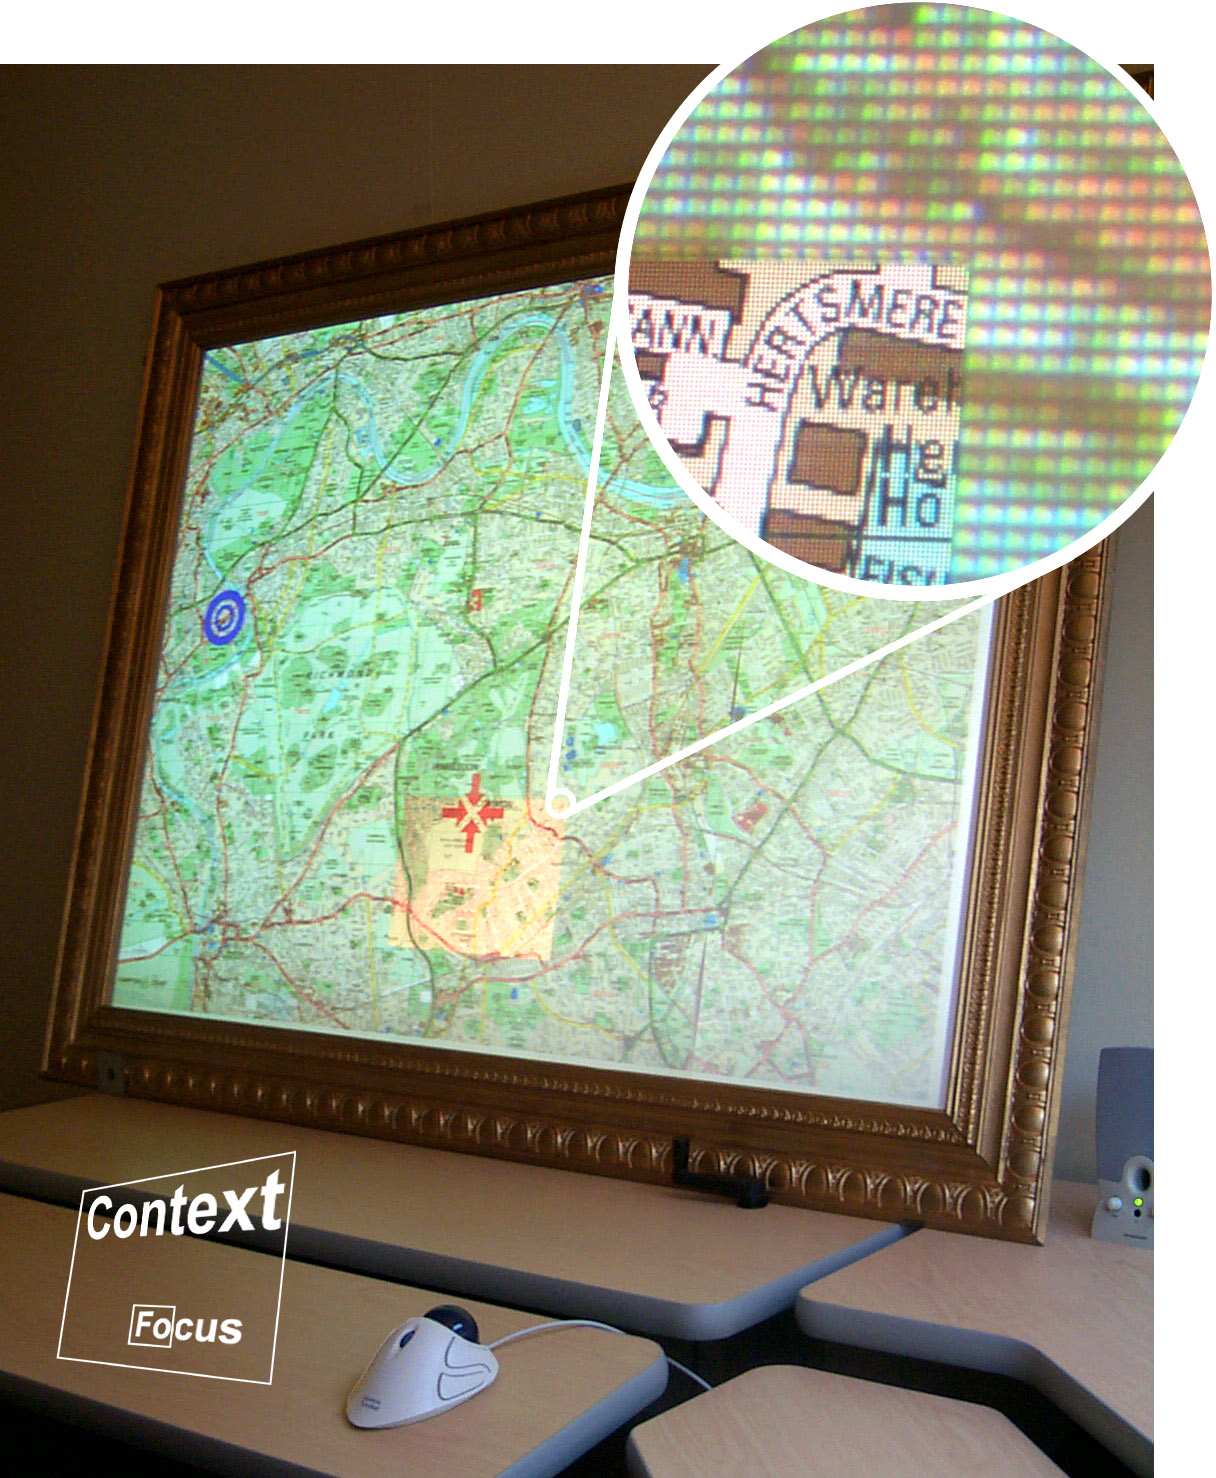
\includegraphics[width=\textwidth]{img/FullsizeMap}
\caption{A focus + context interface. 
The iconic illustration at the bottom left shows where the focus screen is located. 
The callout shows the different resolutions of focus and context area. Source: \cite{Baudisch2002}}
\label{fig:focus_context}
\end{figure}
They demonstrate a display that has an area with higher resolution nested inside a larger area with lower resolution.
A map is presented on the display, with its region of maximal interest (\textit{focus}) inside the area with higher resolution.
One can see that only this small region shows street names.

\todo{Define recognition over recall here?}

\subsubsection{Panning and zooming}
\label{subsubsec:panning_and_zooming}

``\textit{Panning} and \textit{zooming} refer to the actions of a movie camera that can scan sideways across a scene (panning) or move in for a closeup or back away to get a wider view (zooming)`` - \cite{hearst1999modern}.
This is an ubiquitous interaction form that creates a perception of space and movement in said space.
Is in most cases zooming is understood as physical zooming. For comparison with semantic zooming, see \autoref{subsubsec:semantic_zooming}.

\subsubsection{Semantic zooming}
\label{subsubsec:semantic_zooming}

A \textit{physical} zoom changes the size and visible details of objects. 
A \textit{semantic} zoom, on the other hand, changes the type and meaning of the information displayed by the object by using a semantic transition between detailed and general views of information \cite{Modjeska97}.

A thematically relevant example of semantic zooming is presented by Skupin \cite{Skupin2013}.
He automatically derives the thematic structure of a given domain.
As shown in \autoref{fig:som}, he visualized scientific publications from the field of biomedicine.

\begin{sidewaysfigure}[!]
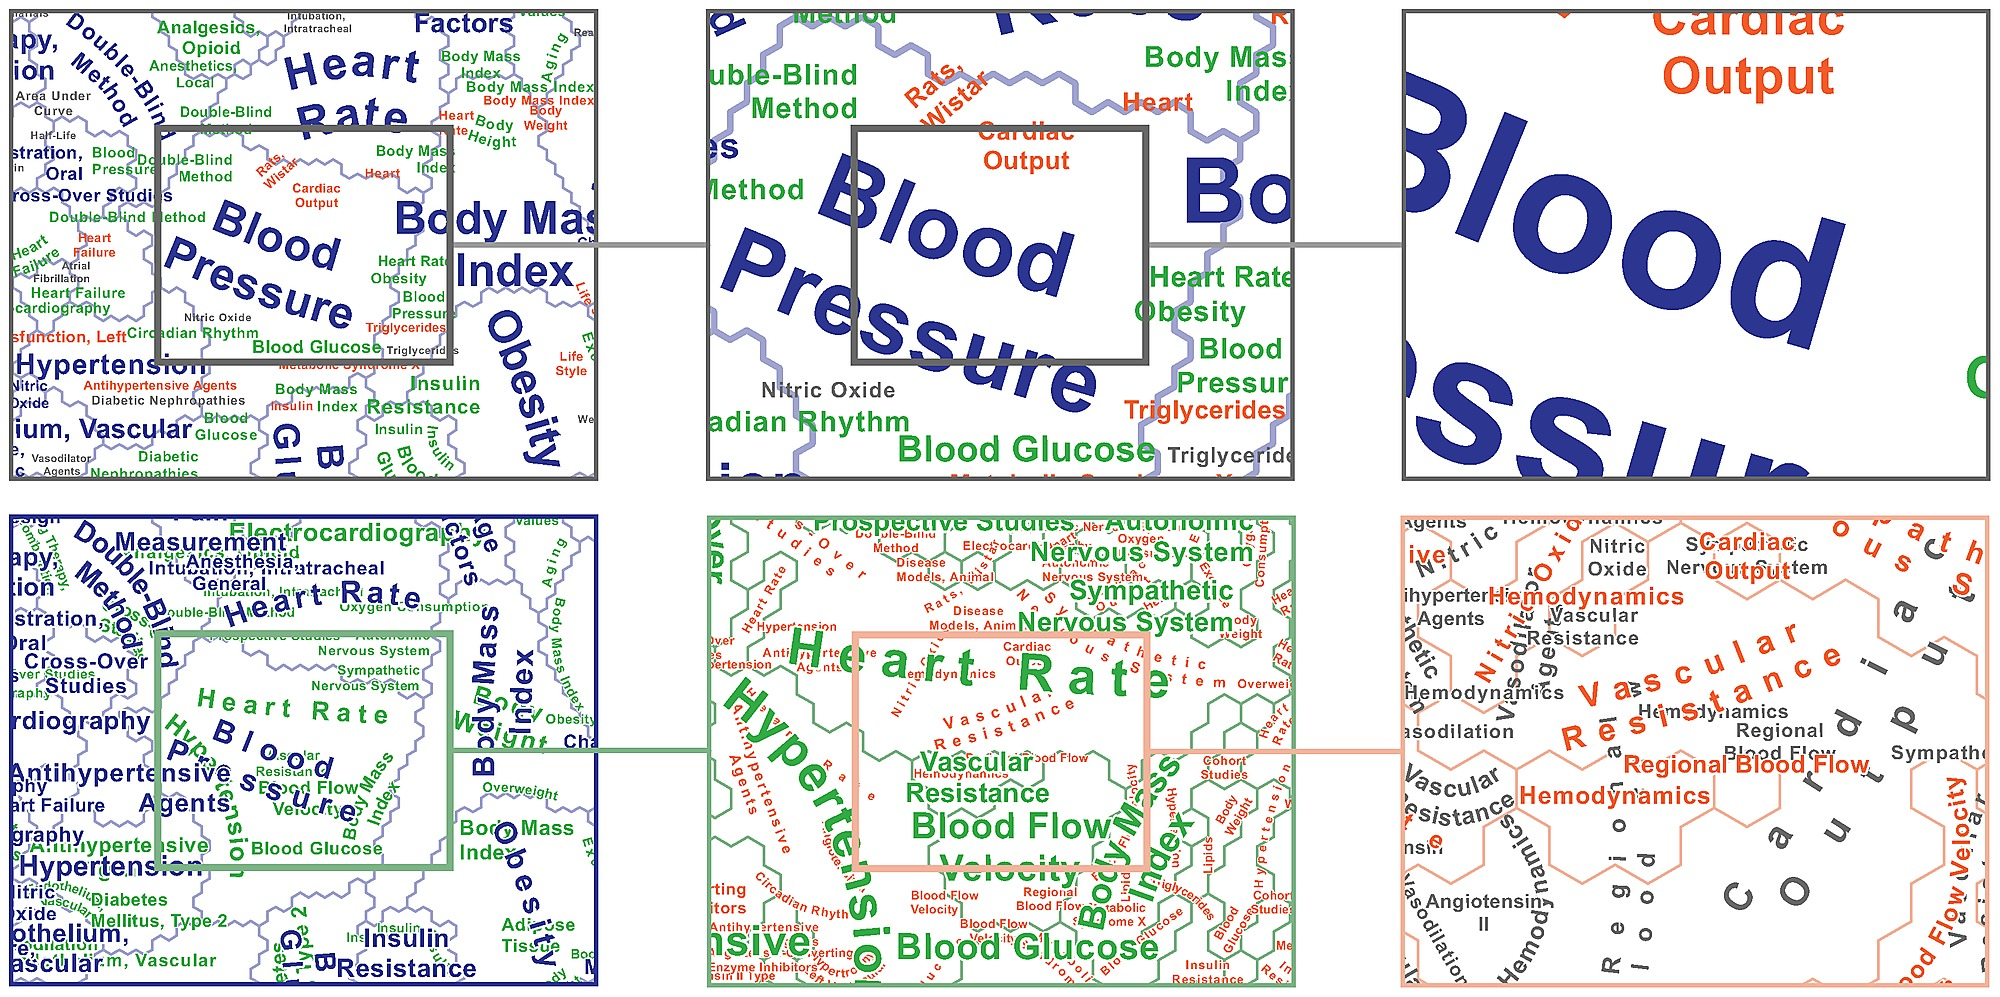
\includegraphics[width=\textwidth]{img/preview}
\caption{Geometric zooming (top) versus semantic zooming with successive revealing of lower levels of term dominance (bottom). Source: \cite{Skupin2013}}
\label{fig:som}
\end{sidewaysfigure}

One can observe that in semantic zooming, the level of detail increases with the zoom level.
Specifically, finer subareas with own labels and boundaries become visible.
Unfortunately, the zooming itself is not implemented in an interactive way in Skupin's case.
Instead, static images are pre-rendered for specific zoom levels.
Deciding when to switch between different levels of detail is a separate problem that we address in our work as described in \autoref{subsec:hierarchical_clustering}.

\subsubsection{Brushing and linking}
\label{subsubsec:brushing_and_linking}

``\textit{Brushing and linking} refers to the connecting of two or more views of the same data, such that a change to the representation in one view affects the representation in the other views as well''  - \cite{hearst1999modern}. 
Multiple views of the same data are usually implemented via different types of visualizations.
Common examples include combinations of scatter plots, bar charts, parallel coordinate views and maps.
Charts do not necessarily need to be of different types.
They may show different dimensions of the data instead (see \autoref{fig:correlation_matrix}).

\begin{figure}[!]
\centering
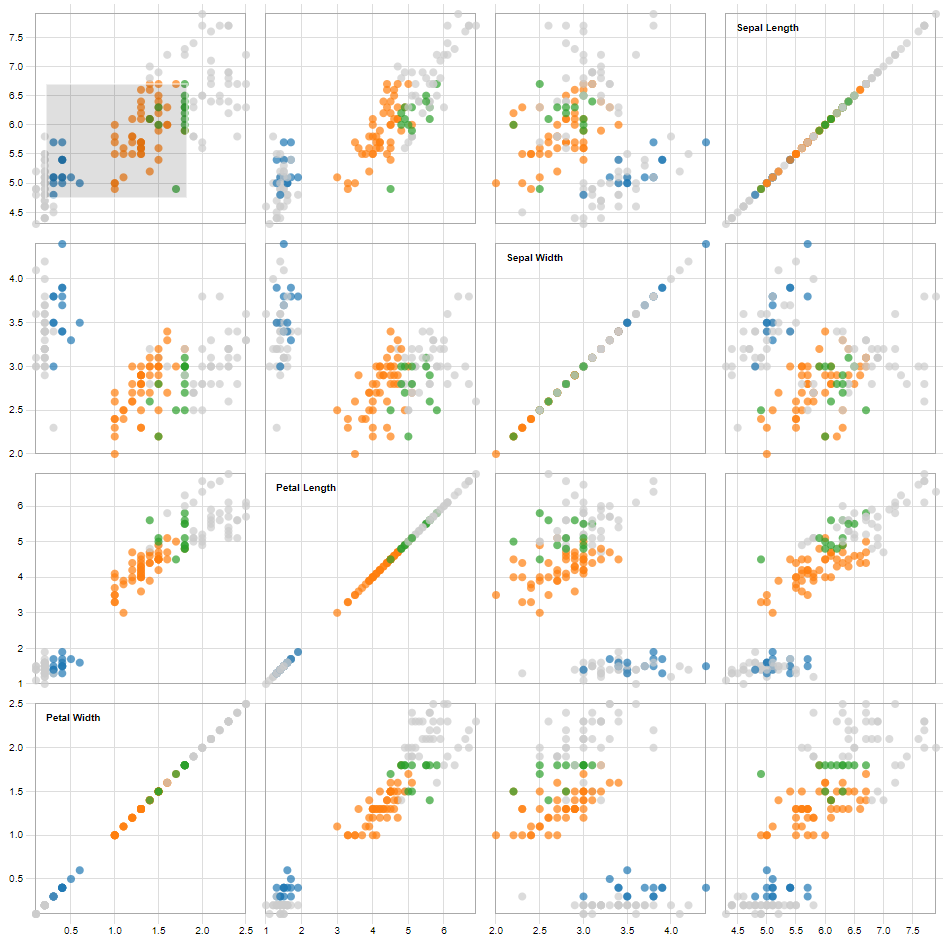
\includegraphics[width=\textwidth]{img/correlation_matrix}
\caption{Correlation matrix of a well-known Iris dataset as an example of brushing and linking. Linked views are all of the same type, which in this case is a scatter plot. Brushed view is in the upper-left corner. Image source and demo: \cite{Bostock2019a}}
\label{fig:correlation_matrix}
\end{figure}

\textit{Brushing} means selecting a part of the data in one of multiple views. 
A selection area is usually formed by dragging the cursor, hence the name \textit{brushing}.
Some form of visual indication is necessary to prevent confusion about what exactly has been selected.
\textit{Linking} refers to highlighting the selected data points in other view or views.
The data is ``linked'' through the selection.
A schematic example of coordinated views with brushing and linking can be seen in \autoref{fig:brushing_linking}.

\begin{figure}[!]
\centering
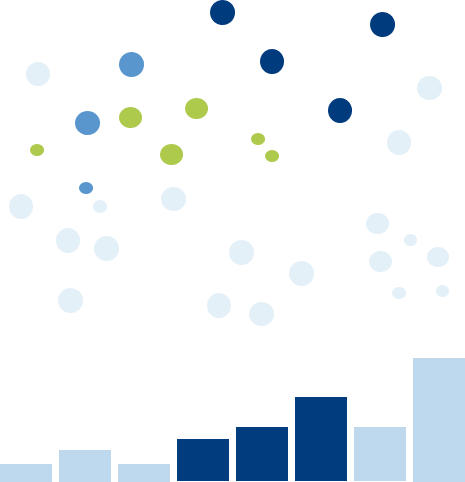
\includegraphics[width=0.4\textwidth]{img/brushing_linking}
\caption{A histogram and a scatter plot coordinated through brushing and linking. The data points that do not belong to the current selection are grayed out in both views.}
\label{fig:brushing_linking}
\end{figure}

\subsection{Machine learning}
\label{subsec:machine_learning}

\subsubsection{Word2vec}
\label{subsubsec:word2vec}

Word2vec was proposed by Mikolov \cite{Mikolov2013}. 
It is a neural network architecture for computing continuous vector representations of words in an n-dimensional space.
The model learns to predict words based on their context.
With enough training data, the hidden layer learns that semantically similar words can be represented with similar vectors.
Those word representations are called \textit{word embeddings} and typically have between 100 and 300 dimensions, while less than 50 dimensions usually don't represent the semantics well enough.

Semantic relationships expressed by word embeddings can be of multiple types.
\cite{Mikolov2013} evaluated semantic and syntactic relationships in question-answer pairs such as city-in-state (i. e. Chicago - Illinois), man-woman (i.e. brother - sister), opposite (ethical - unethical), nationality-adjective (Switzerland - Swiss).
If two words are close in the embedding space, it might also mean that they are synonyms or often appear together in texts.
An illustrative overview of concepts behind word2vec, its training and parameters can be found in \cite{Alammar2019}.

\subsubsection{\gls{tsne}}
\label{subsubsec:tsne}

\gls{tsne} is a dimension reduction technique proposed by \cite{LaurensvanderMaaten2008}.
The aim of the technique is to map high-dimensional data to a two- or three-dimensional space.
At the same time, the structure of the high-dimensional data should be preserved as much as possible.
In other words, \gls{tsne} defines a probability distribution in high-dimensional space and tries to preserve it for low-dimensional space using \textit{gradient descent}.
Gradient descent is an iterative optimization algorithm which aims to find a minimum of a function by taking small steps in the direction of the steepest decline.
The optimization is initialized randomly and is in the case of \gls{tsne} defined by a non-convex cost function, which means that risk of getting stuck in local minima exists.
It is, however, completely acceptable to run the algorithm multiple times and choose the best result.
\gls{tsne} succeeds in preserving both global and local structure of the data, which makes clusters visible at several scales.
An excellent interactive overview of \gls{tsne}'s parameters (especially perplexity) and their influence on resulting behavior of the algorithm can be found in \cite{wattenberg2016how}.

\subsection{Definitions from the patent domain}
\label{subsec:definitions_from_the_patent_domain}

This section contains some basic knowledge about the patent system which is a prerequisite for an understanding of the patent visualization tools related to this work (described in \autoref{sec:state_of_the_art}), and also for an understanding of our own approach (described in \autoref{ch:concept}).
We show how patent documents are structured. 
We also define some terminology from the patent domain that we use throughout this work: patent family, citations and \gls{ipc} classes.

\subsubsection{Structure of a patent document}
\label{subsubsec:structure_of_a_patent_document}

Each patent document possesses the following attributes:
\begin{itemize}
\item \textit{Application number} -  a unique identifier, starts with country code of the registration country. Example: US-5448677-A.
\item \textit{Country code} - stands for the code of the patent office the application was submitted to. 
While some countries, like the US, have their own designated patent offices, there are patent offices, such as the European Patent Office, that allow patents to be valid in multiple countries.
In those cases, terrestrial validity of patents is a complex topic.
For the purposes of simplification, we only consider the code itself (e.g. US or EP) in this work.
\item \textit{Priority date} - the date when the priority patent was submitted (see \autoref{subsubsec:patent_family_and_priority_document} for details on priority).
For our purposes this date is considered as the creation date of the patent.
\item \textit{Assignees} - a list of one or many individuals (inventors) or institutions to which the rights to the invention belong to. It is a categorical attribute.
\item \textit{\gls{ipc} classes} - a list of one or many codes from the \gls{ipc} classification (see \autoref{subsubsec:ipc_classification} for more details) describing the thematic areas of technology the described invention is related to. It is a categorical attribute of a hierarchical nature.
\item \textit{Citations} - a list of patents (identifiable by their application numbers) cited by the given document.
\item \textit{Family identificator} - a number that all members of one patent family share.
\item \textit{Title} - a text attribute describing the invention very briefly . It often does not contain enough useful information if used by itself, but adds some clarity when combined with the abstract.
\item \textit{Abstract} - by analogy with scientific publications, it is a brief summary of the invention.
\item \textit{Claims} - detailed description of the invention and its aspects that should be protected (claimed) by a patent.
This is the field with the most textual information as it can be hundreds to thousands of words long.
Our main data source, Google Patents Public Datasets \cite{IanWetherbee2017}, only provides claims for patents registered in the US.
\end{itemize}

This list is not extensive and only includes fields that are relevant to this work.
For the above-described fields, we distinguish between \textit{textual content} of a document (title, abstract and claims) and the \textit{metadata} which includes all remaining information.

\subsubsection{Patent family and priority document}
\label{subsubsec:patent_family_and_priority_document}

Patents can be assigned to the same \textit{patent family}.
Protection of intellectual property for a patent is restricted to the country the application was submitted to.
Therefore, many inventions are registered in patent offices in multiple countries.
The patents covering one invention across several countries constitute a family.
The earliest patent from a family is called a \textit{priority document}.
Families can also be registered in the same country when they describe different aspects of the same invention.

\subsubsection{Forward and backward citations}
\label{subsubsec:forward_backward_citations}

A patent may include a list of tens to hundreds of citations defined by their application numbers.
When a new patent application cites an already existing patent, it indicates that the cited patent is already known to the applicant \cite{Cotropia2013}.
The older patent in this case is considered \textit{prior art}. 
The new application must provide claims that are novel and non-obvious in the view of the prior art. 
It is in the interest of the applicant to show (through a citation) that they have thoroughly studied already existing patents.
This is analogous to scientific publications where the authors have to review state-of-the-art before proposing novel approaches.

The citations directly defined in a patent, i. e. links to older documents that are being \textit{cited}, are called \textit{forward citations}.
\textit{Backward citations} are the same links from the point of view of the older patent.
They show the patents \textit{citing} the current one.
As it is impossible to know how a patent will be cited in the future, an explicit list of backward citations does not exist and has to be assembled by reversing forward citations.

\subsubsection{International Patent Classification}
\label{subsubsec:ipc_classification}

Each patent is assigned at least one, but usually multiple \gls{ipc} codes.
The \gls{ipc} hierarchy breaks the whole of humanity's patented technological knowledge down into thematic areas the inventions pertain to.
One \gls{ipc} class is an alphanumerical code which is hierarchical in nature and is based on prefixes, i. e. it starts with one letter and with addition of further symbols corresponding new nodes in the hierarchy tree appear.
The tree structure is of the constant depth of five levels and, as we learned in the expert interviews (described in \autoref{subsec:implications}), those levels have own names and are composed according to certain rules (see \autoref{table:ipc_classes_structure}).

\begin{table}[h!]
\centering
\begin{tabular}{||l l l l||} 
 \hline
 Name & Format & Example & Example title \\ [0.5ex] 
 \hline\hline
 Section & One letter & H & Electricity \\ 
 Class & Two-digit number & H04 & Electric communication technique  \\
 Subclass & One letter & H04N & Pictorial communication, e.g. television \\
 Group & One-to-three-digit number & H04N5 & Details of television systems \\
 Subgroup & Two- or three-digit number & H04N5/76 & Television signal recording \\ [1ex] 
 \hline
\end{tabular}
\caption{Structure of \gls{ipc} classes}
\label{table:ipc_classes_structure}
\end{table}

\section{State-of-the-art visualization approaches}
\label{sec:state_of_the_art}

After all prerequisite concepts have been introduces, we review the state of the art with regard to explorative visualization approaches.

Federico et al. \cite{Federico2017} surveyed 21 existing visualization approaches for patents and 109 for scientific documents such as papers, focusing on non-commercially available tools. 
They distinguish between four data types that can be visualized: \textit{text}, \textit{citations}, \textit{authors} and \textit{metadata}.
We focus our review of state-of-the-art on approaches that visualize 1) text alone, 2) other data types alone and 3) text in combination with other data types.
A separate section is devoted to a group of comparable themescape-based approaches.
In the following, a selection of works discussed by Federico et al. is expanded by some other approaches which they did not include.

\subsection{Text-based visualizations}

Johnson et al. \cite{Johnson} present a similar visualization approach to ours with regard to processing the text data for the visualization. 
They use a word2vec model trained on ca. 1.5 million patent texts and compose document embeddings through averaging of word embeddings as well.
They, however, only focus on textual content and disregard visual representation of metadata.
An overview of the whole dataset is not provided.
Instead, one needs to query the data by keywords and only subset corresponding to the query is then shown (see \autoref{fig:johnson}.
The only interaction available apart from querying is the selection of a single patent by clicking on the corresponding point, so that patent details are displayed.
The approach proposes no method to automatically label data points to provide an overview.

\begin{figure}[!]
\centering
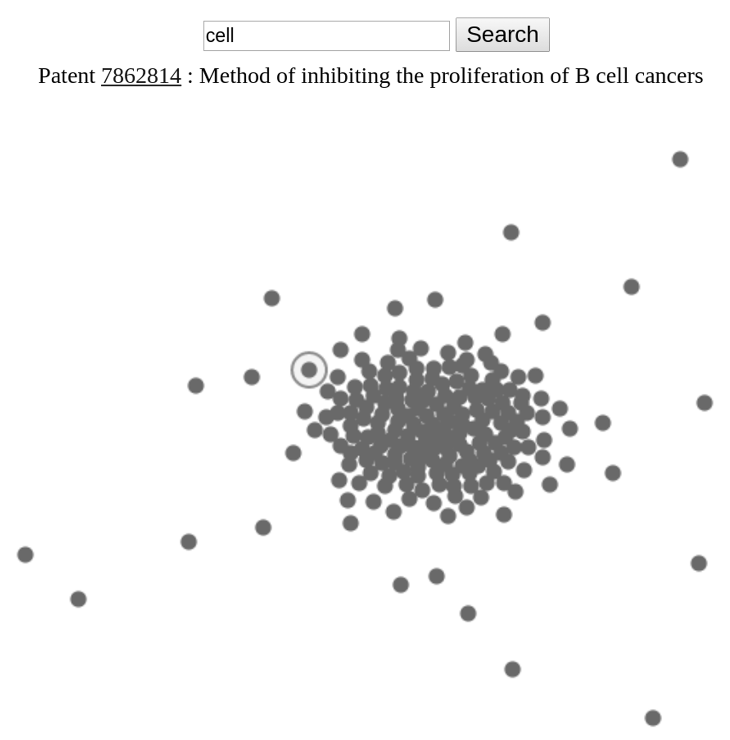
\includegraphics[width=0.5\textwidth]{img/johnson}
\caption{The visualization proposed by \cite{Johnson}. Output of a query for ``cell''. The point in a circle shows the currently selected patent.}
\label{fig:johnson}
\end{figure}

Skupin \cite{Skupin2002} \cite{Skupin2004a} applies a cartographic approach to create maps of non-geographic information, more specifically, conference abstracts.
In a successor work (see Figure \autoref{fig:skupin}), Skupin et al. \cite{Skupin2013} visualize medical publications based on MeSH terms, which are analogous to tags assigned to scientific articles.
In all of those works, a type of \gls{ann} called \gls{som} is used. 
The network is trained on a term-document-/MeSH-document matrix. 
This way, each neuron is assigned multiple terms as labels.
In \cite{Skupin2013}, the neurons are then clustered in the following way: ``if two neurons are neighbors in the two-dimensional neuron lattice and they share the same top-ranked label term, then their boundary is dissolved, thus forming a larger polygon, a neuron label cluster'' \cite{Skupin2013}.
The same procedure is duplicated for the second and third top-ranked label terms, and the resulting three clusterings are then overlaid on the same map and distinguished by color.
Cluster size declines with the dominance of the term, which means the end result displays multiple levels of semantic detail.

\begin{figure}[!]
    \centering
    \subfigure[Zoomed-out view of a complete map of medical literature and detailed views of some regions. Blue, green and red labels indicate clusters derived from the first, second and third top-ranked label term, respectively. Source: \cite{Skupin2013}]
    {
        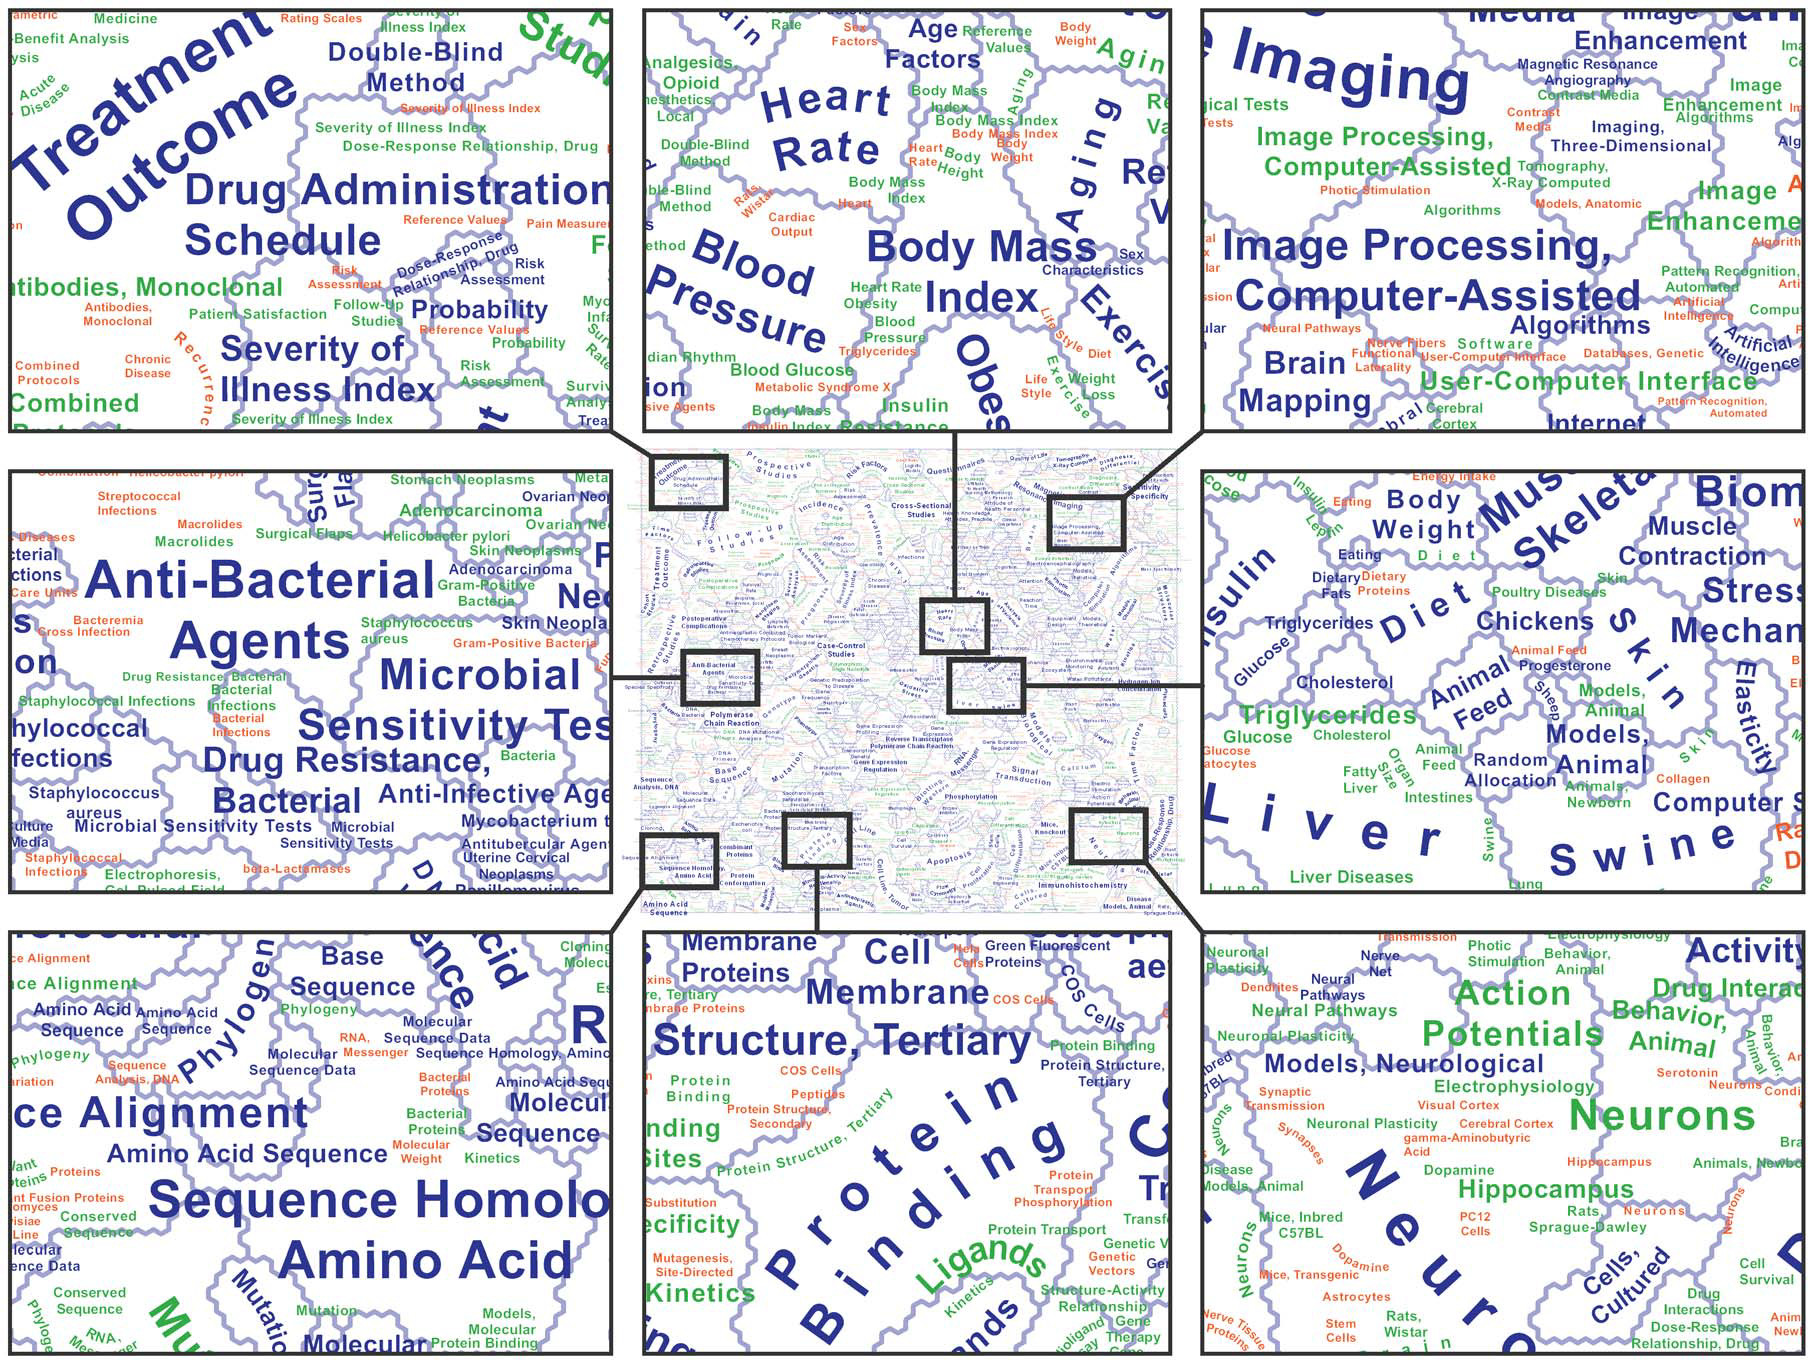
\includegraphics[width=\textwidth]{img/skupin}
        \label{fig:skupin}
    }\\
    \subfigure[Visualization of conference abstracts with simultaneous overlay of three levels of a hierarchical clustering. Source: \cite{Skupin2002}]
    {
        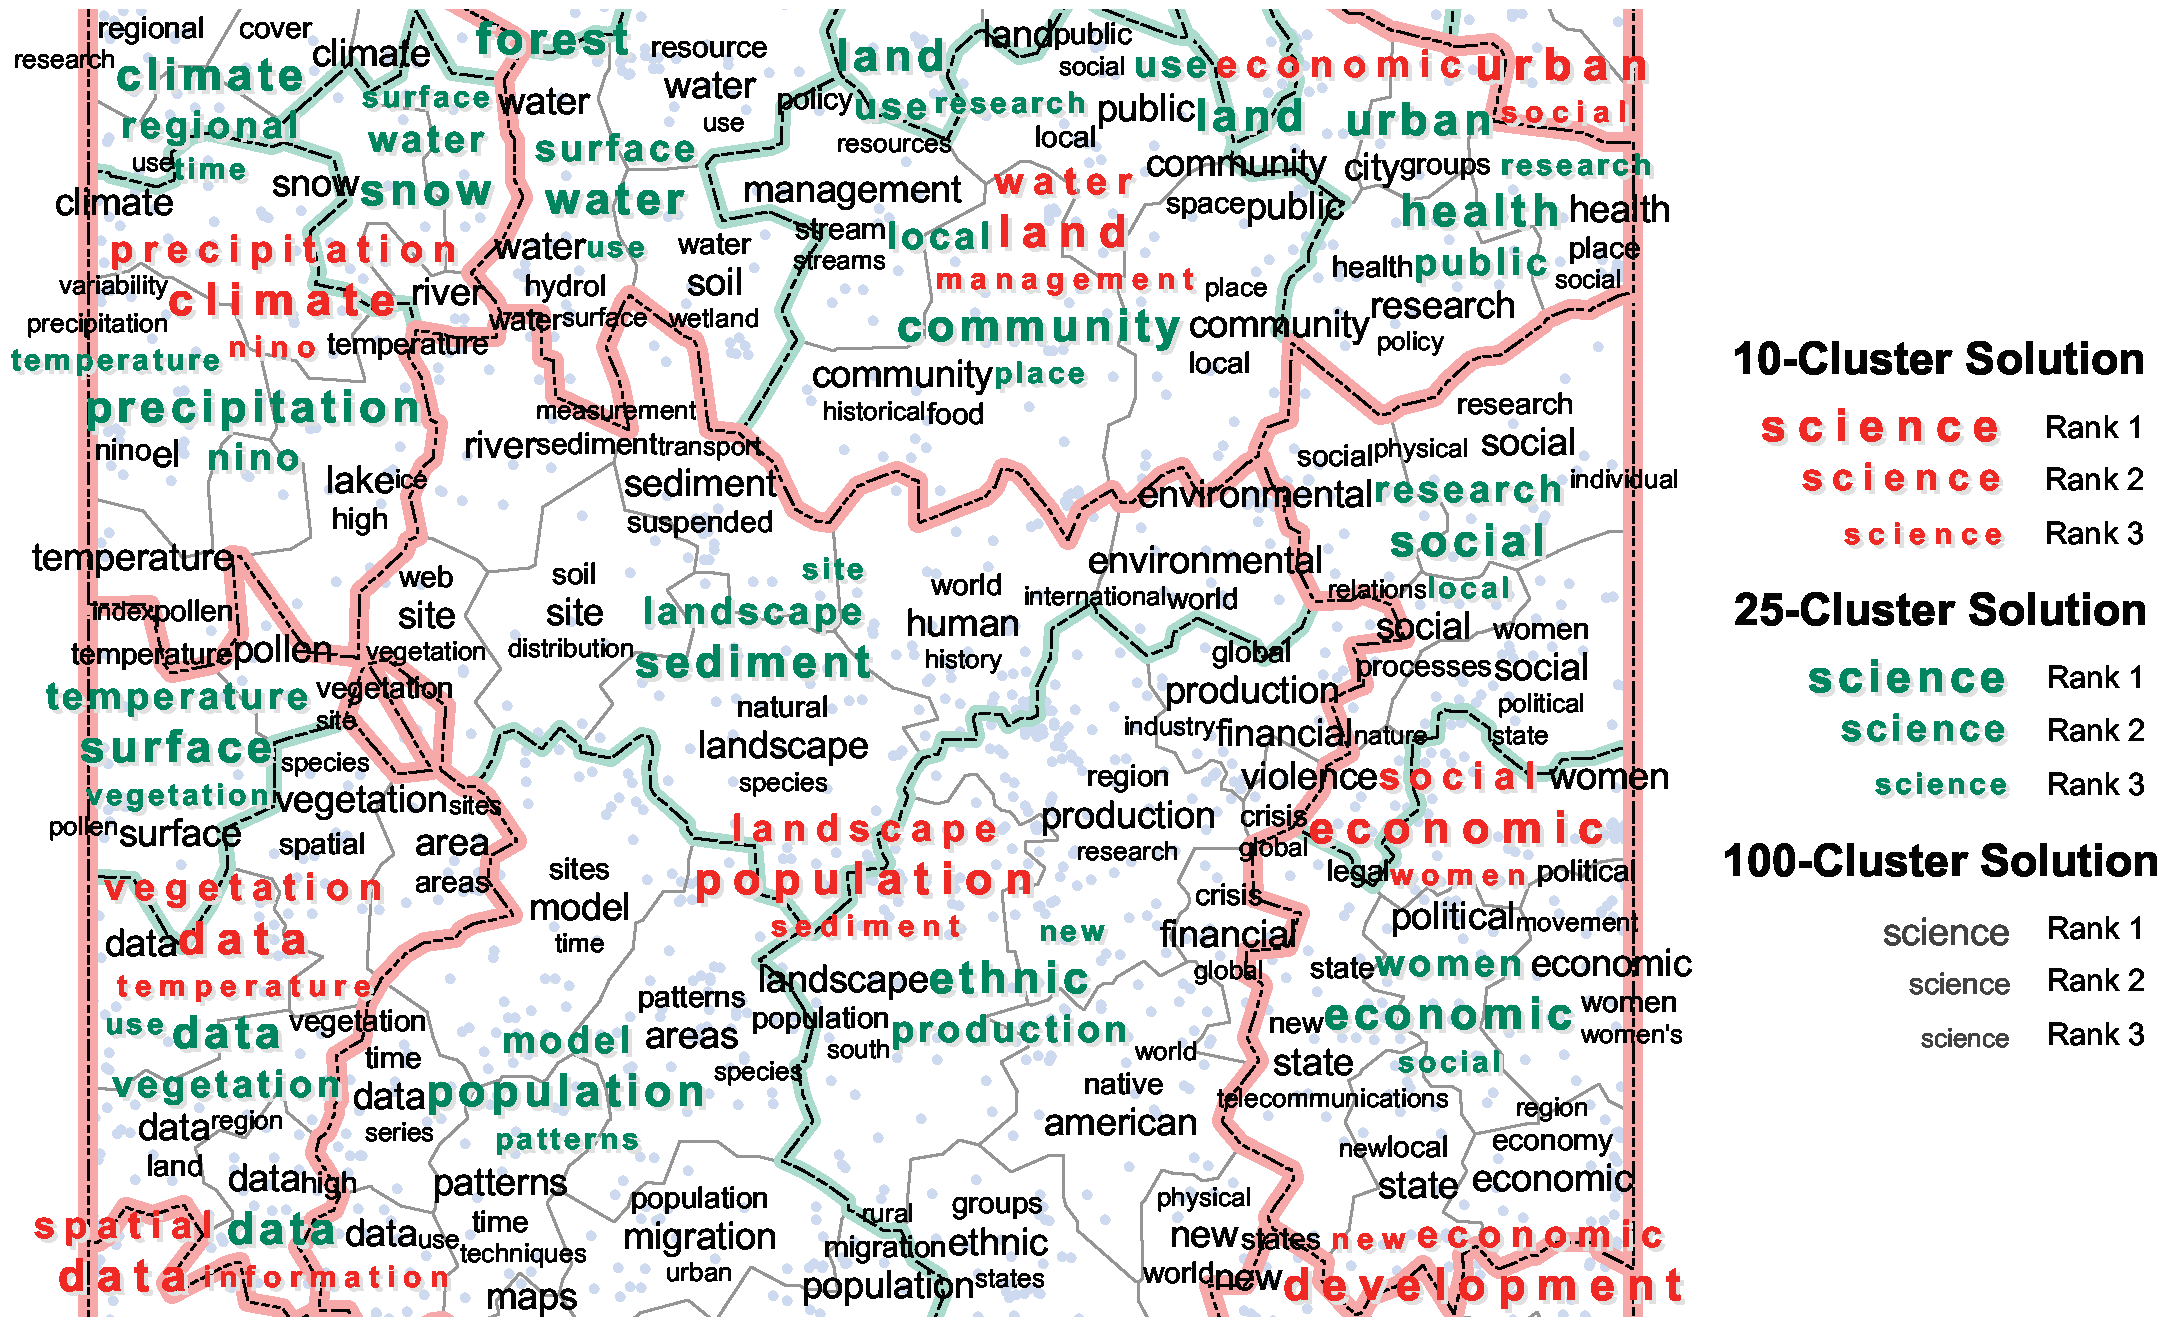
\includegraphics[width=\textwidth]{img/skupin1}
        \label{fig:skupin1}
    }
    \caption{Skupin's maps of knowledge domains}
    \label{fig:skupin_all}
\end{figure}

In \cite{Skupin2002} and \cite{Skupin2004a}, Skupin uses an alternative clustering method - hierarchical clustering.
From the tree structure built on neuron similarities he derives three to five clustering levels as shown in Figure \autoref{fig:skupin1}.
This approach served as an inspiration for our own hierarchical clustering based on similarities between patent documents.

Our approach builds upon Skupin's ideas and aims for a comparable result, while the features of the data and the processing methods are different.
Visualizations proposed by him are either static or provide a basic zooming interaction while limiting the richness of display.
We, on the contrary, specifically focus on supplementing a hierarchical themescape with interactivity for effective exploration.

Choo et al. \cite{utopian} present UTOPIAN (\textbf{U}ser-driven \textbf{T}opic modeling based on \textbf{I}nter\textbf{a}ctive \textbf{N}onnegative Matrix Factorization).
They perform topic modeling based on a bag-of-words representation of a document.
A hard-clustering algorithm is then applied to the documents, which means that each document is assigned to only one topic.
A modified version of \gls{tsne} is utilized to draw a node-link diagram with topics/clusters distinctly separated as shown in \autoref{fig:utopian}.
Edges are drawn between pairs of data points whose distances are below a user-specified threshold.
Most importantly, the approach gives the user a high level of control over the topic modeling result.
Merging or splitting topics, creation of a new topic based on a specified document or a certain keyword are possible.
Choo's approach influenced our initial idea of drawing a fully connected graph of documents which would dynamically reform itself after some documents are filtered out (see \autoref{subsec:initial_concept} for details).
We, however, did not pursue this idea further because of performance considerations.

\begin{figure}[!]
\centering
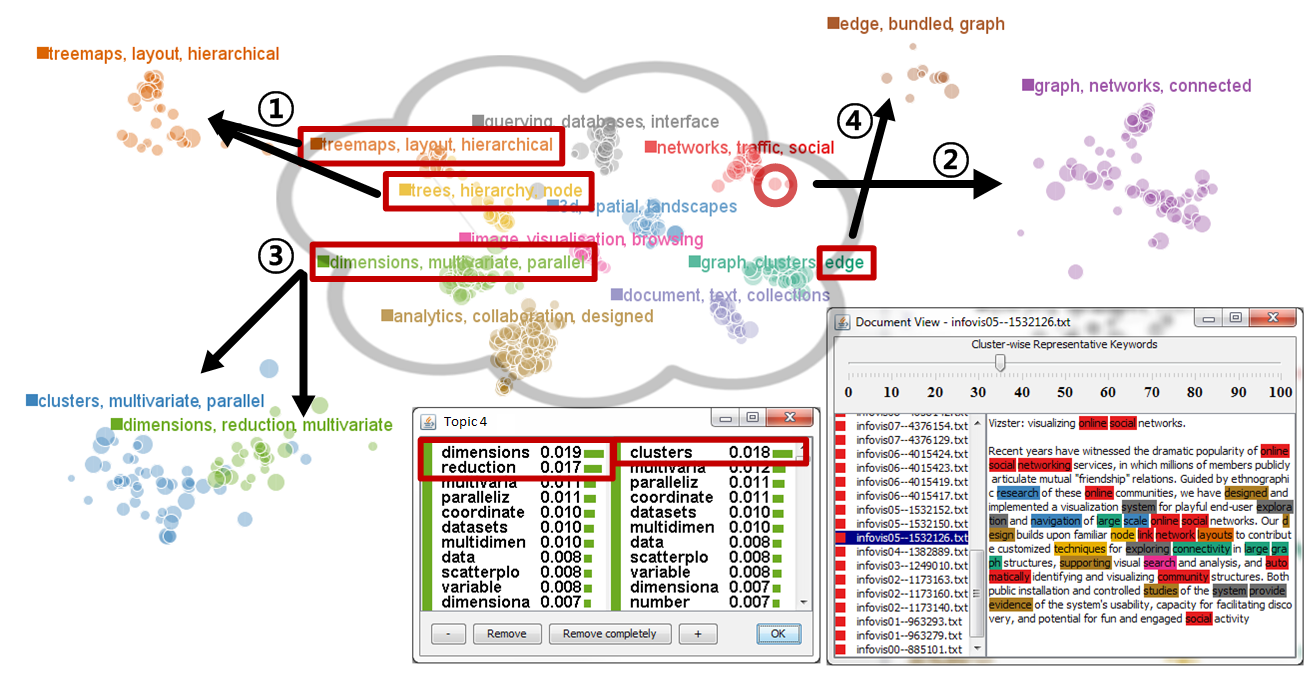
\includegraphics[width=\textwidth]{img/utopian}
\caption{UTOPIAN by \cite{utopian}. Given a scatter plot visualization generated by a modified \gls{tsne}, it provides capabilities for 1) topic merging, 2) document-induced topic creation, 3) topic splitting and 4) keyword-induced topic creation. The user can adjust topic keyword weights (bottom-middle) and see representative keywords in the document viewer (bottom-right).}
\label{fig:utopian}
\end{figure}

\subsection{Visualizations based purely on metadata}

Patent data is distinguished by a significant amount of metadata attached to each record: hierarchical classification, assignees, citations, patent family information, etc.
Many works deal with one or a number of these attributes \cite{Zhao2013} \cite{Wittenburg2015} \cite{Herr2014a} \cite{Giereth2007} \cite{Garfield2004} \cite{Chen2004} \cite{abello}.
However, Federico et al. emphasize that “only few works adopt, refine, or develop techniques for visualizing classification data. Other data types are just ignored in most approaches” \cite{Federico2017}.
Because of this, we aim to derive value specifically from the hierarchical representation of \gls{ipc} classification data.

Wittenburg et al. \cite{Wittenburg2015} make extensive use of metadata for faceted visualization with what they call embedded bar charts.
They order the company, decade of filing date, country and \gls{ipc} class vertically over each other and represent the distribution of values within those attributes through widths of blocks as seen on \autoref{fig:wittenburg}.
The embedded bar charts use negative space within the blocks to display temporal development of a company's patenting behavior.
Unfortunately, Wittenburg's approach results in a cluttered view and therefore lacks visual scalability when many companies and especially \gls{ipc} classes are present in the data.
Nevertheless, we build upon their idea about displaying distributions of metadata attributes in a stacked order.

\begin{figure}[!]
\centering
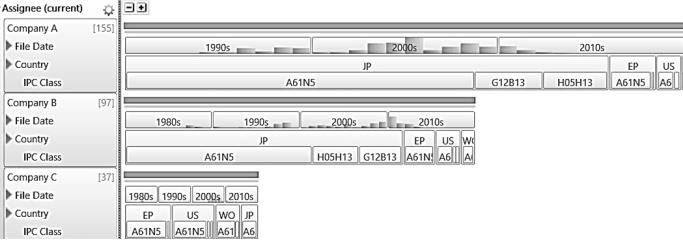
\includegraphics[width=\textwidth]{img/wittenburg}
\caption{A visualization layout proposed by \cite{Wittenburg2015}, a so called embedded bar chart. The distribution of metadata attributes in the dataset is represented by a hierarchy of attributes: assignee, then date of filing, then country, then \gls{ipc} class.}
\label{fig:wittenburg}
\end{figure}

\subsection{Visualizations based on text in combination with other data types}

%User interaction provides immense added value in the task of finding patterns in data. 
%However, Federico et al. note that most visualizations only made limited use of interaction techniques such as detail-on-demand, focus + context or coordinated multiple views. 
%This research gap needs to be addressed specifically because interaction plays a big role in tackling the challenge of scalability for the steadily increasing number of text documents.

Many approaches capture thematic similarities between documents with help of topic modeling \cite{nakazawa} \cite{gretarsson} \cite{Dou2011} \cite{Jiang2016}.
They position a document depending on the degree to which it belongs to the corresponding topic.
For example, Dou et al. \cite{Dou2011} uses the parallel coordinate metaphor to present a probabilistic distribution of a document across pre-detected topics as seen in \autoref{fig:dou}.
With an interactive ThemeRiver view they present the temporal development of the topics.
Lastly, they use a scatter plot to show the distribution of single-topic vs. multi-topic documents.
Pie glyphs within the scatter plot describe the topical contribution to a specific document.
We consider the parallel coordinate plot a suboptimal choice to represent a large number of similar dimensions such as >10 topics.
Even though the topic axes are ordered by similarity, the positive and negative correlations between topics become spread over the >10 vertical axes, which makes them hardly perceptible.
Nevertheless, this approach served as an inspiration for our own glyphs in the form of a pie chart.

\begin{figure}[!]
\centering
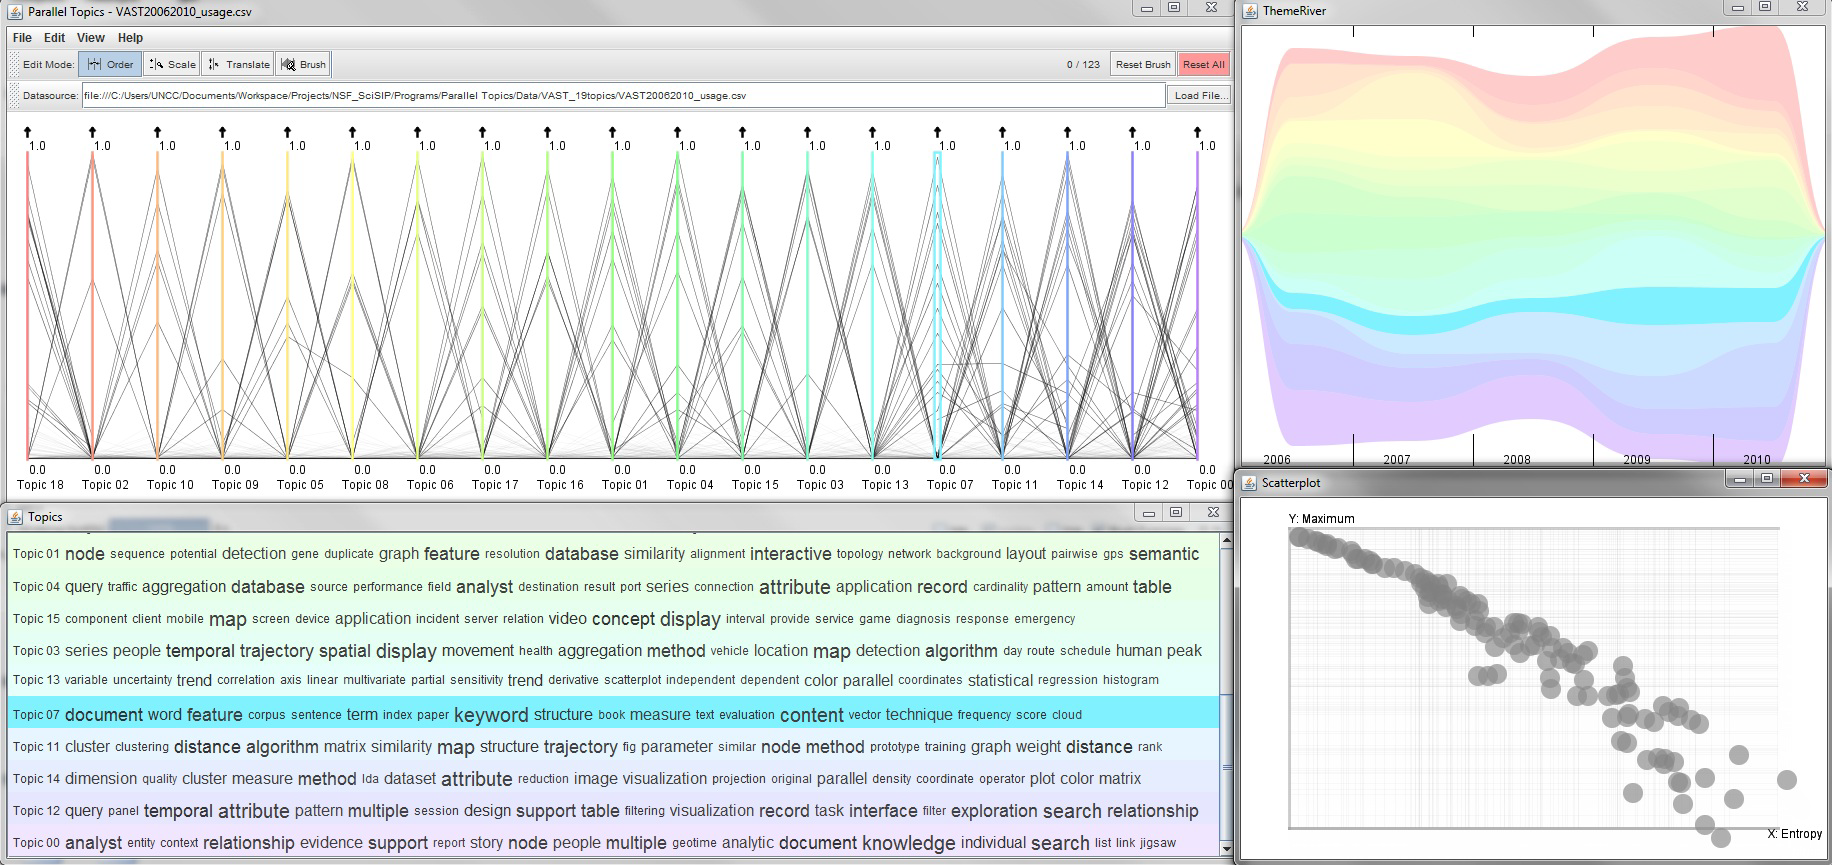
\includegraphics[width=\textwidth]{img/dou}
\caption{ParallelTopics by \cite{Dou2011}. Top left: Document Distribution view, top right: Temporal view, bottom left: Topic Cloud, bottom right: Document Scatterplot.}
\label{fig:dou}
\end{figure}

Jiang et al. \cite{Jiang2016} present a comparable approach to Dou et al. as seen in \cite{fig:jiang}.
They detect tens of topics using a hierarchical topic model.
Each topic is then represented as a vocabulary-length feature vector where each dimension corresponds to the word's probability in a latent semantic space.
The topic vectors are then reduced to two dimensions via \gls{mds} and are shown in the form of a scatter plot.
This approach comes close to our idea of making patterns in the semantic space visible.
Unfortunately, it does not provide a representation of how separate documents relate to topics.
It also involves only the temporal dimension of documents and no as an addition to their textual content, no other metadata is represented.

\begin{sidewaysfigure}[!]
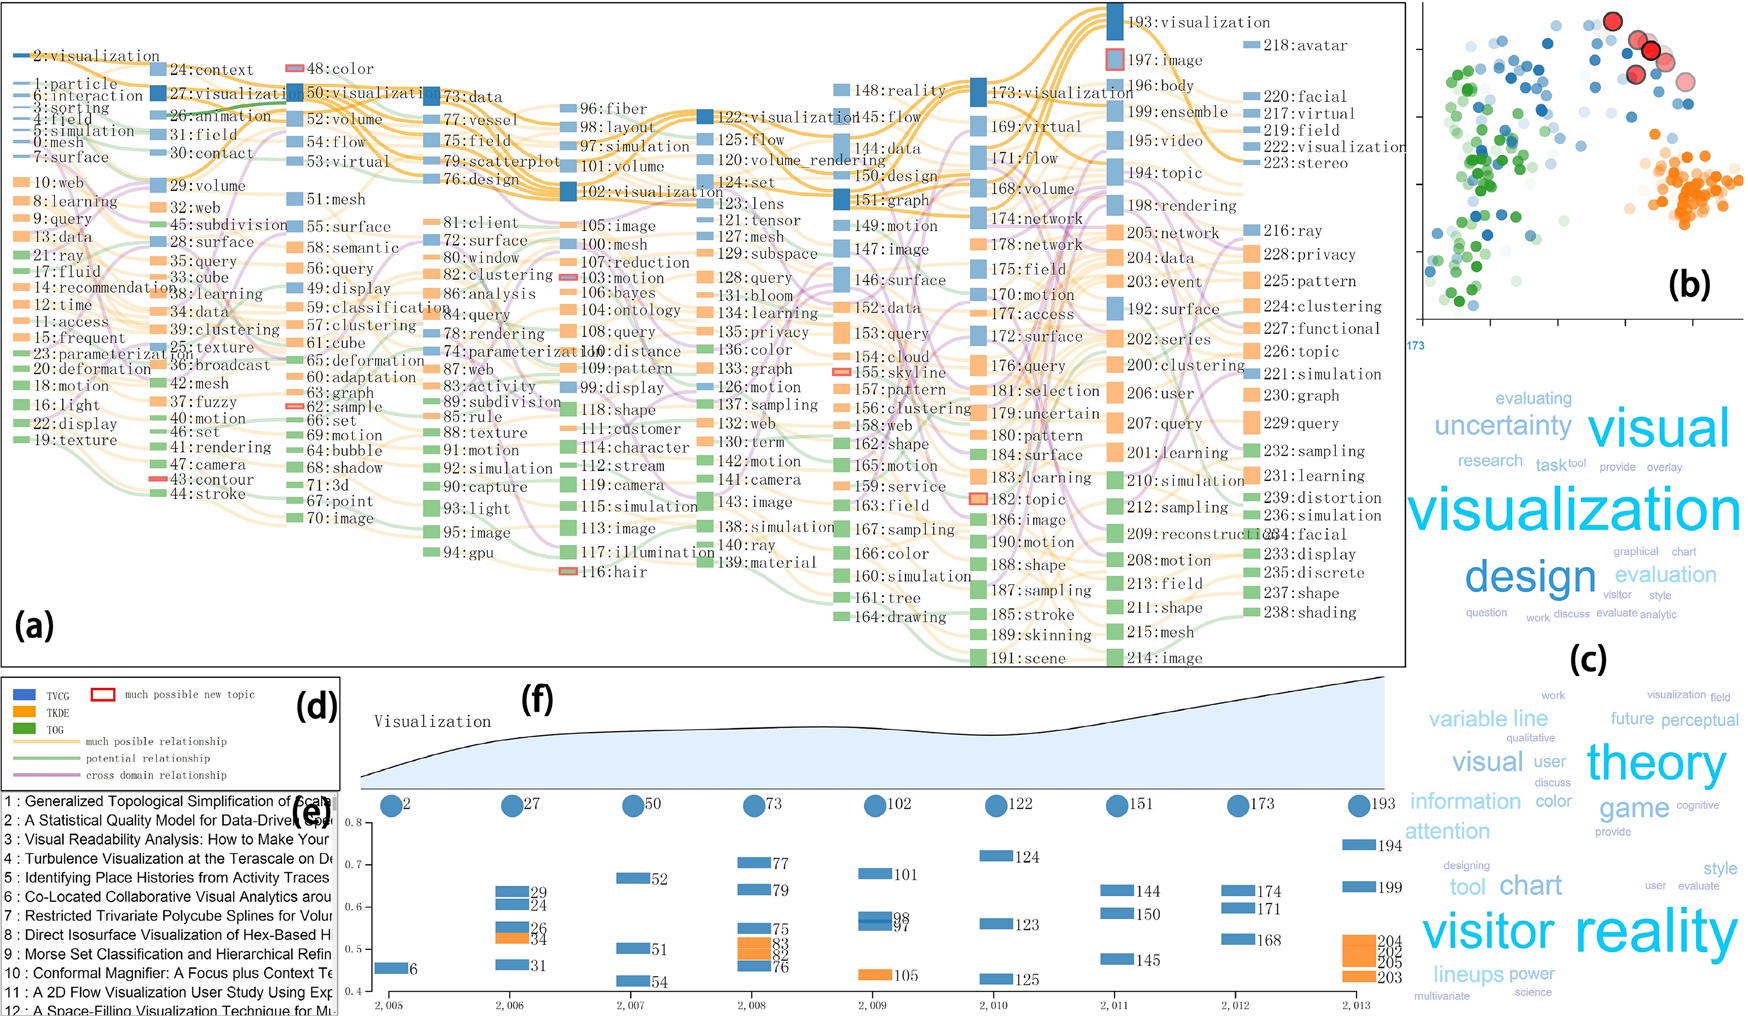
\includegraphics[width=\textwidth]{img/jiang}
\caption{A visualization approach by \cite{Jiang2016}. a) sankey diagram presenting the temporal development of numbered topics; b) scatter plot showing the topics in 2D space; c) word cloud of the selected topic and subtopics;  d) legend; e) titles of papers belonging to the selected topics; f) stream diagram illustrating the topic trend with a scatter plot to represent topic similarities. }
\label{fig:jiang}
\end{sidewaysfigure}

\subsection{Themescapes}
Visualization approaches that produce themescapes constitute a separate noteworthy category.
They include commercial tools such as VxInsight \cite{Boyack2002}, Thomson Reuter’s Aureka and STN's AnaVist.
Information about those tools is limited because of their cost, but \cite{Ruotsalainen2008} provides an extensive comparison.
There are also some non-commercial approaches such as IN-SPIRE \cite{hetzler}. 
All of those approaches utilize the metaphor of points in a landscape comprised of ``mountains'' and ``valleys'' as seen in \autoref{fig:aureka}.
Mountains group patents with similar textual content via word-frequency-based similarity metrics.
The height of a mountain peak corresponds to the document density in the area.
A peak is usually labeled with a list of automatically extracted relevant terms.
Skupin's work takes advantage of the map metaphor as well, but does not completely fit into this category because he does not use the third dimension to represent the amount of documents in a cluster.

In most themescape-based approaches, the user can highlight points on the landscape which correspond to a certain author, patent assignee, time period, country, etc.
Thus, a distribution of metadata values can be explored.
Moreover, coordinated views supplement the main landscape view by providing statistics in form of histograms, co-occurrence matrices, pie charts, citation graphs, etc. (see \autoref{fig:anavist} for an example from AnaVist).

The little information that is publicly available about the commercial themescape-based tools seems to indicate that all of them use document representations based on frequency and/or distribution of words.
In such classical machine learning methods, words are treated like indices in a dictionary and there is no concept of context or similarity between words.
In our work we compare one such approach (\gls{tf-idf} document vectors) with a newer neural-net-based approach that takes semantics of words into account.

\begin{figure}[!]
\centering
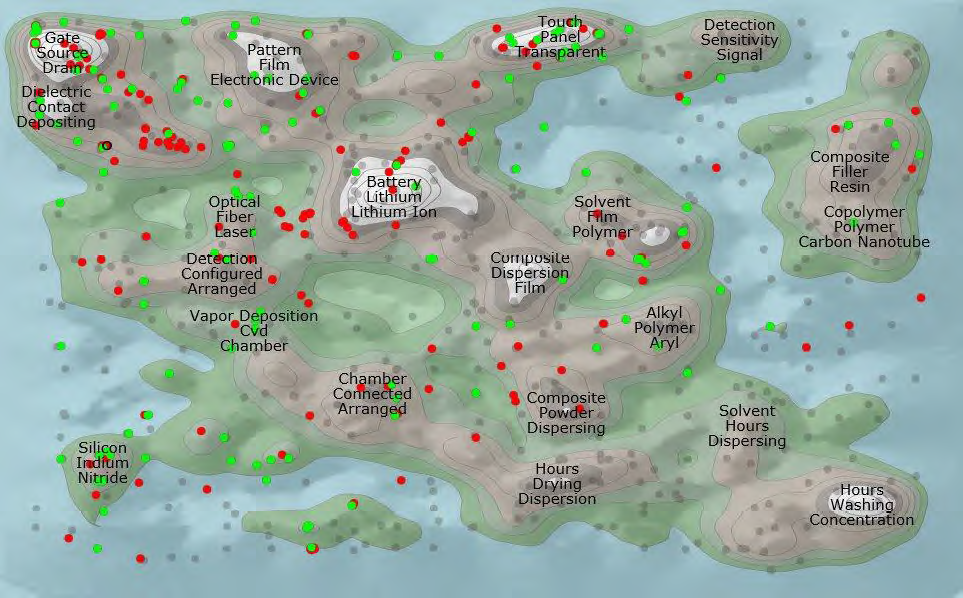
\includegraphics[width=\textwidth]{img/aureka}
\caption{A patent landscape map about graphene produced with Aureka. Highlighted are Samsung's patents published in 2013 and 2014. Image source: \cite{graphene}}
\label{fig:aureka}
\end{figure}

\begin{sidewaysfigure}[h!]
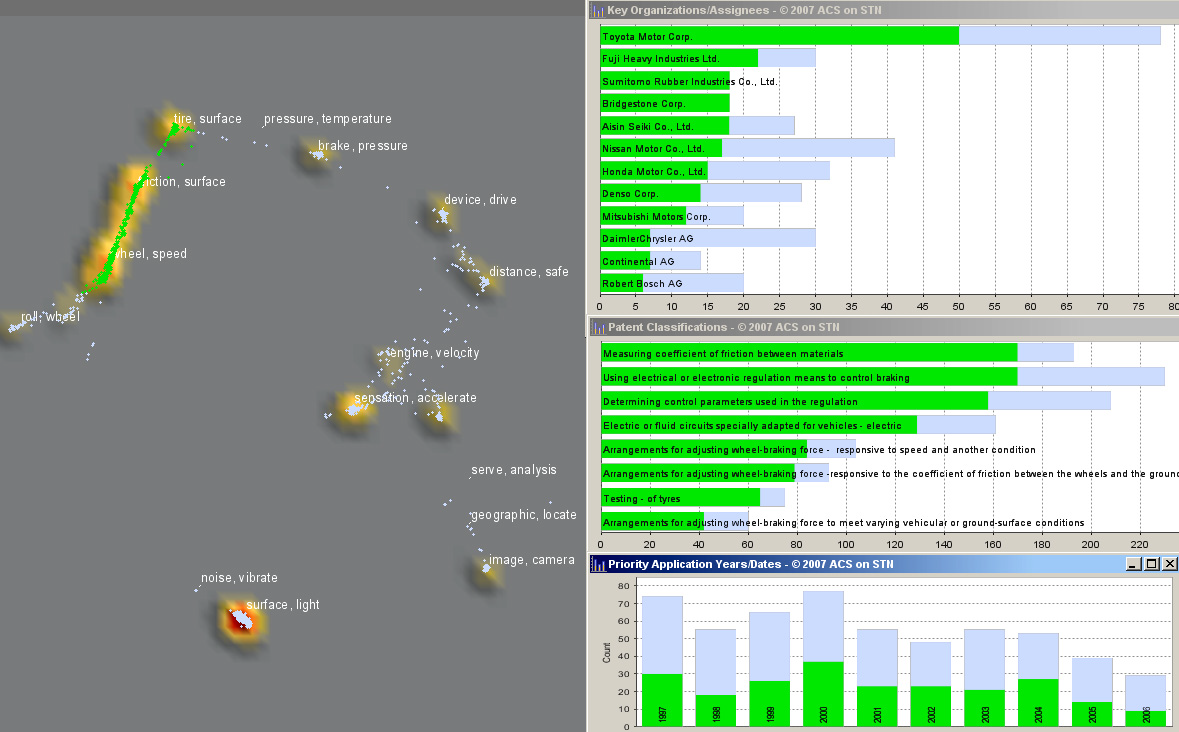
\includegraphics[width=\textwidth]{img/anavist}
\caption{Screenshot of STN AnaVist, a commercial tool for patent landscaping. A selected subset of the data is highlighted in green. Image source: \cite{Ruotsalainen2008}}
\label{fig:anavist}
\end{sidewaysfigure}

\subsection{Summary}

Many approaches use topic modeling as a way to give meaning to the positions in the visualization space.
Others use similarity metrics based on word frequencies to cluster documents.
Only one approach (Federico et al. \cite{Federico2017}) uses semantic word embeddings instead of word-frequency-based features.

Very few works handle patent classification data, which is why we explicitly focus on finding an appropriate visual metaphor for \gls{ipc} classes.

Ultimately, we are unaware of any approach that 1) relies on semantic embeddings to show local and global structures within a dataset, 2) organizes themes into a conceptual hierarchy via clustering and at the same time 3) enables exploration of document metadata through additional visual dimensions or interaction techniques.
This is the research gap we address in this work.
%% LaTeX2e class for student theses
%% sections/content.tex
%% 
%% Karlsruhe Institute of Technology
%% Institute for Program Structures and Data Organization
%% Chair for Software Design and Quality (SDQ)
%%
%% Dr.-Ing. Erik Burger
%% burger@kit.edu
%%
%% Version 1.3.3, 2018-04-17
\chapter{Case study}
\label{ch:case_study}

After we have covered the basic concepts and reviewed the existing visualization approaches, we define the framework for the case study which directs our solution and, later, helps to evaluate it.

\section{Design of case study}
\label{sec:design_of_case_study}

A \textit{case study} is an empirical method aiming at investigating contemporary phenomena in their context. 
While it does not uncover causal relationships as well as a controlled experiment would, it provides deeper understanding of the studied phenomenon and is flexible \cite{Runeson2009}.
Nevertheless, a case study has to be carefully planned.

\subsection{Plan for the case study}
\label{subsec:plan_for_case_study}

According to \cite{robson2002real}, a plan for a case study has to include:
\begin{itemize}
\item Objective—what to achieve?
\item The case—what is studied?
\item Theory—what is the frame of reference? 
\item Research questions—what to know?
\item Methods—how to collect data?
\item Selection strategy—where to seek data?
\end{itemize}

In this section we answer those questions.

Tools already exist to support exploration of corpora of text documents in general and the patent landscaping process specifically.
Therefore, the case study has an \textit{improving} objective.

The objective and the research questions of this work have already been covered in detail in \autoref{sec:objectives}.

The \textit{case} that is being studied is the task of patent landscaping.

The study operates under the assumption that semantic embedding results in a similarity measure that is meaningful for human perception. 
This assumption defines the \textit{frame of reference}.

Next, methods for data collection and data selection strategy have to be defined.
We use \textit{first degree} data collection techniques, more specifically, user interviews and a think-aloud study complemented by a \gls{sus} questionnaire.
The participants for those studies are experts from the patent domain.

\textit{First degree} data collection techniques are methods in which the researcher is in direct contact with the subjects and collects data in real time\cite{Lethbridge2005}.
Second and third degree techniques mean collecting data without direct participant interaction or using data that already exists, respectively.
A comparison of techniques of various degrees of access can be seen in \autoref{fig:degree_techniques}.

\begin{figure}[h]
\centering
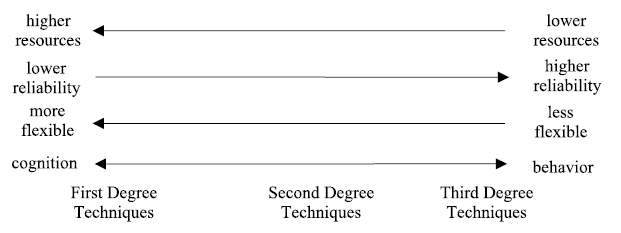
\includegraphics{img/degree_techniques}
\caption{Cost, reliability, flexibility and cognition vs. behavior compared. Source: \cite{Lethbridge2005}}
\label{fig:degree_techniques}
\end{figure}
First degree techniques require more time and effort from both researcher and study participants.
This is due to the fact that they tend to produce a large amount of data that needs processing.
On the positive side of this trade-off, first degree techniques provide the researcher with more flexibility and control over data collection.
Most importantly, first degree techniques allow the researcher not only to understand \textit{how} the task is performed (behavior), but \textit{why} (cognition).
The downside is that the gathered data relies on imperfect human recollection, so care must be taken if complete accuracy of reported facts is important.
Since we are interested in overall cognitive processes instead of minutia, we implement first degree techniques in our case study.

\subsection{Procedures for data collection}
\label{subsec:procedures_for_data_collection}

After having settled on using first degree data collection techniques, in this section we define how the data is to be collected.
This includes a detailed discussion of the user studies that produce the data to collect.

\paragraph{Formative study}~\\
First, a formative study in the form of expert interviews serves to understand scenarios in the patent landscaping task and formulate the requirements. 
The purpose of this first stage of data collection is to acquire subjective, qualitative results since actual human experiences provide valuable insight into benefits and drawbacks of existing solutions. 
Accordingly, \textit{semi-structured} interviews are chosen to understand the users’ mental model of the task.
A semi-structured interview consists of a mix of open and closed questions.
This type of interview is common in case studies \cite{Runeson2009}.
It allows the researcher to follow the natural development of the conversation, improvise and explore the subject at hand while making sure that all relevant topics are addressed.
We discuss the results of the formative study in \autoref{sec:interviews}. 

\paragraph{Ideation}~\\
After the first data collection stage, a concept for the visualization itself must be developed. 
The concept is influenced by the insights gained in the formative study. 
The result of the decisions made at this stage is a digital mockup representing the future interactive prototype (see \autoref{ch:concept} for details).
An implementation phase that follows consists of data preprocessing, applying chosen semantic methods and implementing chosen interaction techniques in a usable interactive prototype (see \autoref{ch:implementation} for details).
After the first proof-of-concept prototype is complete, a short feedback meeting with the potential users takes place .
This helps gather first reactions to the concept and, when necessary, adjust further iterations.

\paragraph{Summative study}~\\
An evaluation of the approach is concluded by the second data collection stage.
The execution of this stage is covered \label{ch:evaluation}.
One of the purposes of the second data collection stage is to uncover cognitive problems and mismatches between the user's mental model of the task and the proposed system.
The second purpose is to evaluate the impact of semantic embeddings as compared to a traditional approach such as \gls{tf-idf} features as document vectors. 
To do that, participants are divided into two groups. 
One group evaluates the traditional approach first and the approach with semantic embeddings afterwards. 
For the second group, the order is reversed.

To gather direct qualitative feedback about usability, a think-aloud study is planned.
The think-aloud approach has its roots in cognitive psychology and is scientifically established \cite{Simon2006} \cite{Ericsson1980}.
It was originally applied in studying short-term memory processes.
Two embodiments of the think-aloud method exist. Ericsson et al.
\cite{ericsson1984protocol} keeps the influence of the experimenter on the outcome to a minimum with rigid procedures.
Contrarily, \cite{Boren2000} et al. approach the experiment as a dialogue.
The participant is still encouraged to talk most of the time.
The researcher mostly listens and acknowledges what is being said, but is allowed to ask questions or intervene in case the participant is lost or a bug in the tested system prevents further progress.
The two techniques were evaluated in \cite{Krahmer2004}.
The outcome shows that the subjects' evaluations were consistent between methods.
However, the subjects completed more tasks and felt less lost with approach from Boren et al.
We therefore choose this embodiment of think-aloud for the qualitative part of our summative study.

For quantitative feedback, we measure the usability score resulting from the use of the prototype.
This helps verify that the visualization based on the proposed approach is easy to use and satisfies the requirements.
For that, \gls{sus} questionnaire \cite{Brooke1996} is chosen.
It is preferred to other questionnaires such as \gls{csuq} \cite{Lewis1993} and \gls{quis} \cite{Chin2003} because it produces reliable results even with small number of participants \cite{Tullis2004}. 
Moreover, it is short, simple and addresses different aspects of user's reaction to the tested system as a whole instead of its specific features.
Alternating positive and negative questions (``I thought the system was easy to use'' vs. ``I found the system unnecessarily complex'') require attention from participants and provide more robust results.
\cite{Laubheimer2018} proposes to combine a \gls{sus} scale with a follow-up question about reasons for the given rating to derive further qualitative insights. 
We follow this suggestion. 

\paragraph{Study subjects}~\\
Experts with experience in patent landscaping from FIZ Karlsruhe serve as subjects of the study. 
According to Nielsen \cite{Nielsen2000}, about 70\% of the insight can be learned from three participants.
Additional participants, especially those after the fifth one, bring merely diminishing returns. 
For this reason, the study is kept small with 3 participants for user interviews and 4 for the think-aloud and \gls{sus} part.

Analysis of the data collected during the second data collection stage allows drawing conclusions regarding the objectives of the study.
Those are described in \autoref{sec:discussion}.

\section{Interviews}
\label{sec:interviews}

Since the formative study defined in the previous chapter had a direct impact on the development of our approach described in \autoref{ch:concept}, we cover the study itself and its results in this section.
First, we describe the organizational and methodological aspects of conducting a semi-structured interview, which is an integral part of the formative study.
After the organizational and methodological aspects follow the descriptions of conversations with patent experts.
We conclude by a summary of how the interviews shaped our understanding of the patent domain and, subsequently, how they influenced the development of a concept for our approach.

\subsection{Procedure}
\label{subsec:procedure}

Three patent experts were interviewed in a semi-structured format as defined in \cite{robson2002real}. 
After greeting the participant, each interview started with some warm-up questions about participant's background. 
Afterwards followed the main part with the most important questions about the domain of patent landscaping itself.
The interview was concluded by cool-down phase with more general questions.
The questions covered relevant aspects of a patent landscaping process such as data quality, usage scenarios and working with different abstraction levels.
A full questionnaire for the interview can be found in \autoref{sec:semi_structured_interview_questionnaire}.

Best practices for conducting user interviews were studied and adopted to the best of interviewer's ability.
Here we list the guidelines that we followed based on \cite{Portigal2013}:
\begin{itemize}
  \item Before scheduling the interview, ask participants if you are allowed to record them talking.
  It is virtually impossible to actively listen and steer the conversation while taking extensive notes.
  An audio recording is usually sufficient.
  Don't forget to check recording equipment before first interview starts.
  \item The questions should not assume a certain point of view. 
  For example, ``How do you feel about X?'' is better than ``Why is X bad?''.
  Ask even if you think you know the answer, you might be surprised.
  \item Show that you understood what the interviewee is saying and ask for clarification. 
  For example, ``You said X, could you please tell me more about it?''.
  \item If questions come up while the interviewee is speaking, don't interrupt them. 
  Write the question down and follow up later.
  \item Speak slowly, don't show hurry.
  If the time is running out, prioritize.
  \item Pay attention to interviewee's body language and try to imitate it when appropriate. 
  Try to prevent defensive poses such as crossed arms.
  \item Leave long pauses after the interviewee's replies.
  Silence is mildly uncomfortable and serves as a prompt to keep talking.
  It also gives the participant a chance for contemplation, allowing them to formulate additions to their last thought.
  \item After the main part of the interview is finished, ask the participant if they have questions for you or would like to tell you something you both had not discussed yet.
  \item After completing the interview thank the participant, stop the recording and note the main topics of the conversation.
\end{itemize}

All participants were to some degree familiar with STN AnaVist, which is an interactive visualization software specifically created for use in the patent domain.
As seen in \autoref{fig:anavist}, it displays a patent map with labeled clusters and allows the users to select an area to compute statistics about the patents in that area as compared to the whole dataset.
Prior exposure to STN AnaVist most probably shaped experts' expectations for a patent landscaping tool.
%Moreover, in their daily work routine the experts use non-visual /move to discussion

The interviews provided valuable insights into workflows and mental processes of patent experts. 
In the the descriptions of the conversations we only elaborate on discussion points that are relevant to the development of our approach. 
The issues not covered here nevertheless significantly contributed to our understanding of the patent domain.

We refer to the participants by the letters of the Greek alphabet and singular ``they'' for both genders to preserve their anonymity.
The grammatical form of singular ``they'' also applies for any (potential) users we mention throughout this work.

\subsection{Participant Alpha}
\label{subsec:participant_alpha}

Participant Alpha has the most experience with patent landscaping.
They composed patent landscape reports and are very familiar with the landscaping tool STN AnaVist and presented it to clients.

Participant Alpha characterized creating a patent landscape as an iterative process. 
It consists of multiple feedback loops that run until converging to a satisfactory result.
 
The first feedback loop involves understanding the needs of the client better. 
It starts when a client commissions a patent analysis and explains their requirements to the expert.
The mutual understanding of the task is difficult to achieve, especially when it evolves based on illustrative results. 
Therefore, after the patent expert presents the client with the result of the current iteration, the client may influence the focus of the analysis.
The expert incorporates the client's suggestions into the further workflow.

The second feedback loop concerns the level of abstraction in the query to the patent database.
Participant Alpha pointed out that the patent attorneys often use very generic vocabulary compared to scientific publications such as papers.
This allows the claimed invention to be protected in a wider variety of embodiments.
Patent offices work against this tactic by demanding a sufficient level of detail to prevent claims from being too broad.
As a result, patent expert sometimes has to experiment with making terms of the search query more or less generic.
If a query consists of parts A, B and C, a combination of generic search terms for A and B and specific terms for C might be followed by a combination of specific terms for A and C with generic terms for B.
Thus, possible combinations of generic and specific terms for parts of the query are tested iteratively until the query result is satisfactory.
The optimal level of detail for each part of the query constitutes a substrategy, and such substrategies are merged in the final query.

Participant Alpha highlighted the importance of uniform names for assignees and inventors. 
They reported a recent ``information flood'' from Asia, especially from China, which necessitates uniform rules for transliterating proper nouns.
According to the participant, uniform names of patent assignees are a distinguishing feature of high-quality datasets that is required by clients.
Non-uniform names make aggregating data, i. e. counting, unreliable.

The participant made a distinction between two kinds of patent landscaping.
One involves looking at a patent set in a quantitative way through the set of metadata attributes.
It helps answer questions such as who are the biggest competitors, since when they have been active, how many applications do they have, in which countries are they active.
The second kind involves better understanding of the technology domain and ability to subdivide it into subdomains.
The participant named freedom-to-operate research as a possible scenario for this kind of analysis.
In this area they saw potential for use of semantic methods such as the contribution of this thesis.

The participant described multiple definitions of a patent family. 
The most widely accepted one and also the broadest one is ``simple family'', which constitutes a group of patents associated with the same priority document.
Simple family may contain patents with claims that differ significantly because they protect different parts of the same invention or take into account regional differences.
Creators of patent databases such as Derwent also create their own definitions of family which are more narrow and typically contain almost identical patents only.

Aside from the freedom-to-operate scenario, the participant also mentioned 1) whitespot analysis, 2) searching for cooperation partners and  3)``licensing out'' patents that are not in company’s core portfolio as valid scenarios where a patent landscaping tool has successfully been used or might be useful.
If one searches for a widespread technology, whitespots can be recognized where a few data points are on their own and not in any big cluster.

Participant Alpha emphasized strongly the importance of data quality. 
They reported that a patent in a full-text database might be about 100 pages long, while same patent in an added-value database, such as Derwent, might be about 2 pages.
This difference is explained by the fact that texts in an added-value database are rewritten by professional writers to a more concise and understandable form.
Added-value databases are used as a default option during a patent search.
Full-text databases are only searched when necessary.

While on the topic of patent classification systems, participant Alpha reported that \gls{ipc} is used by virtually all patent offices worldwide and covers about 98\% patent documents.
Though \gls{cpc} has more meaningful and better structured hierarchy, it is assigned to only 40\% of documents and is therefore unreliable if used by itself.
The participant named subclass level (i. e. A61K), main group (i. e. A61K6) and subgroup (i. e. A61K6/02) as most widely used levels of the \gls{ipc} hierarchy.
Some \gls{ipc} codes are assigned consistently and are suitable for searching using \gls{ipc} codes only, while others require searching with help of key terms. 

\subsection{Participant Beta}
\label{subsec:participant_beta}

Due to their background, this participant has some experience in text mining, especially annotating patent texts.
Accordingly, initial questions led to a detailed discussion on this topic.

Participant Beta pointed out that machine translation, \gls{ocr} artifacts and different writing styles make automatic analysis error prone.
Participant Beta repeated Participant Alpha's assertion about quality of the data playing a crucial role in automated analysis.
The participant elaborated that sometimes the user might get an impression of some trends happening, while in reality they only can be attributed to the noise and errors in the data.

According to Participant Beta, it is difficult to separate citations from the rest of the text, and noise in data occurs when this process was not successful. 
Nevertheless, assuming that citations were recognized successfully, they constitute a very important kind of connection between documents and represent a very strong similarity. 
If A cites B, but they do not have similar key terms, the approach might be faulty.
Patent families should be grouped in an obvious way as well.

Considering usage scenarios, Participant Beta reported that in 80\% of all cases solely the distribution of assignees plotted by publication year was sufficient.
Moreover, participant expressed doubt about value of visual patent landscaping tools compared to traditional non-visual tools.
The participant themselves as well as other patent experts have difficulty interpreting the visual representation of a landscape.
The connection between terms that describe clusters is perceived as far from obvious and needs an explanation.
The meaning of valleys between the mountains in tools such as STN AnaVist is also confusing.
It is unclear to patent experts how one is supposed to recognize patterns and draw conclusions from such representation and what additional knowledge it provides.
Dislike for black-box algorithms was expressed by the participant and their acquaintances.

The participant provided some advice concerning processing of the textual content.

First, they recommended using patent title and abstract together because the title itself might be too short (i. e. one word) or not expressive enough.

Second, they advised to pay special attention to stopword removal. 
There are stopwords that apply for all English texts, such as ``is'', ``have'', etc. 
Stopwords specific to patent domain include structural markers such as ``patent application'', ``description'',  ``prior art'' or``claim''. 
The participant reported that during demonstrations of patent analysis software, they have regularly seen stopwords which should have been removed.

Third, Participant Beta highlighted the importance of not only single-word key terms but phrases that are two or three words long.
Such phrases may consist of nouns but also of adjectives and participles.
However, the participant's impression was that single-word key terms do not appear sufficiently often after key term extraction.
The participant disapproved of this, because some domains possess highly relevant one-word key terms. 
The situation was attributed by the participant to insufficient weighting by the extraction algorithm.

Participant Beta stated that the description field in a patent can be separated into multiple segments such as ``Background of the Invention'', ``Summary of the Invention'', ``Brief Description of the Drawings'', ``Detailed Description of the Preferred Embodiment'' and ``Claims''.
The segmentation is not a straightforward process because the format of the parts of the description varies significantly.
Assuming the segmentation is successful, ``Summary of the Invention'' and ``Detailed Description of the Preferred Embodiment'' provide most value.
The participant expressed curiosity to compare results of a semantic approach between the above-named description segments and ``Background of the Invention''.

\subsection{Participant Gamma}
\label{subsec:participant_gamma}

Participant Gamma had most experience with very specific questions from clients that needed quite specific answers. Typical size of a query result for them is 30-50 patents from which about 5 most relevant have to be selected and presented to the client.

Participant Gamma repeated statements from Participant Alpha about the iterative nature of a patent search. 
They both described the process in a very similar way: one should approach a search from multiple perspectives, develop multiple strategies and merge them at the end.

Participant Gamma explained that freedom-to-operate research needs very complete answers to the search query.
It is very important that no relevant patents are missing from the dataset, otherwise absence of any already protected inventions cannot be proven.

When it comes to working with single patent documents, the workflow is as follows. 
First title and abstract are read. When those are interesting enough, the full text is requested (which might require an additional fee) and studied. 

Participant Gamma echoed Participant Alpha's sentiment about limited usefullness of \gls{ipc} classes. 
For broad analyses they are found helpful, while the more specific the search becomes, the more weaknesses \gls{ipc} shows.

Due to the very narrow nature of requests Participant Gamma works on, they did not see data visualization as the main tool for the search task for them personally.
Instead, they saw it as a way to generate impressive visuals for the stakeholders or other non-experts. 
Nevertheless, they admit that visualization may be useful when dealing with large datasets. 
In this case, interaction and usable filtering features are seen as very important.
Participant Gamma acknowledged that demand for such patent visualization tools exists among their clients.

\subsection{Findings from user interviews and their implications}
\label{subsec:implications}

In this section, we briefly summarize the findings from the user interviews and how they influence our approach:
\begin{itemize}
\item Thematic consistency of IPC classes declines as one moves to the lower levels of IPC hierarchy. 
It also varies a lot depending on the specific technology domain.
One therefore should not expect a clear separation of classes in the semantic space during the clustering (see \autoref{subsec:hierarchical_clustering} for details) and the evaluation (see \autoref{ch:evaluation} for details on evaluation).
Nevertheless, patent experts work with all levels of IPC hierarchy.
\item Names of assignees (companies or individuals a patent belongs to) are often spelled differently throughout the dataset.
This makes grouping patents by assignee name unreliable.
Disambiguated assignee names are one of the characteristics of a quality dataset.
We therefore merge assignees with similar names via fuzzy string matching as a part of the preprocessing before we aggregate the documents (see \autoref{subsec:data_preprocessing} for details).
\item Patent language differs in form and structure from the common written language. 
Both general and very specific vocabulary is used in patent texts, and, accordingly, in patent searches.
Consequently, we use a language model trained specifically on patent texts because it reflects the peculiarities of the patent domain best.
We then attempt to produce generalizations of cluster key terms as described in \autoref{subsec:hierarchical_clustering}.
\item Special attention has to be paid to the elimination of stopwords that add no value to the general understanding. We describe the process of the stopword removal and the stopword lists we use in \autoref{subsec:data_preprocessing} ``Stopword removal''.
\item Patent's title is rarely sufficient to describe its content and thus should be considered together with the abstract. 
The ``Description'' field of a patent consists of segments that vary in relevance and are difficult to separate.
Since our data source does not provide a segmented description, we use another textual field named``Claims'' instead as described in \autoref{subsec:data_preprocessing}.
\item In patent-specific language there are a lot of established expressions that consist of multiple words.
This means it is not sufficient to only extract single-word key terms, which is why we extract both unigrams and bigrams to characterize content of patent documents and document clusters as described in \autoref{subsec:term_extraction}.
\item Belonging to the same patent family constitutes the strongest kind of connection between patents.
In most cases, patents from the same family should be adjacent in the semantic space.
At the same time, families with diverging content exist where this rule of thumb does not apply.
We use proximity of patent families as a minimal criterion which has to be met in the visualization space (see \autoref{subsec:embeddings} for details).
\end{itemize}
%% LaTeX2e class for student theses
%% sections/content.tex
%% 
%% Karlsruhe Institute of Technology
%% Institute for Program Structures and Data Organization
%% Chair for Software Design and Quality (SDQ)
%%
%% Dr.-Ing. Erik Burger
%% burger@kit.edu
%%
%% Version 1.3.3, 2018-04-17

\chapter{Visualization concept}
\label{ch:concept}

In the previous chapter we described how the interviews with the patent experts shaped our understanding of the patent landscaping task.
The knowledge gained in the process combined with the ideas gained from state-of-the-art approaches allowed us to develop a concept for the visualization.
In this chapter, we first outline the visualization concept in its final state.
We then cover the decisions that led to this stage.
Lastly, a brief summary of the data processing steps needed to produce document representations is given.
In the next chapter (\autoref{ch:implementation}), we present the separate components of the user interface of the visualization and of the data processing pipeline in their implemented form and discuss them in detail.


\section{Outline}
\label{sec:outline_visualization_concept}

In this work, we deal with semantic exploration of documents.
This refers to, on the one hand, the challenge of displaying high-dimensional \textit{semantic representations} of documents visually.
On the other hand, we support \textit{semantic interactions}, which means that the display adapts to the intentions of the user with regard to information density and level of detail.
These two topics are reflected in our concept.

A simplified representation of the visualization layout can be seen in \autoref{fig:schematic}.
The user interface consists of four interconnected parts: scatter plot, histogram, detail view and sunburst including breadcrumbs.

\textit{The scatter plot} is the main area of the visualization where each patent document is represented as a point.
Visualization space within the scatter plot is, effectively, the high-dimensional semantic space reduced to two dimensions. 
The user can navigate this space by panning and zooming (see \autoref{subsubsec:panning_and_zooming} for details on panning and zooming).
Each document is labeled by its relevant key terms which are extracted as described in \autoref{subsec:term_extraction}.
To keep the point labels readable, a heuristic is applied for optimal text density depending on the number of points within view and the zoom factor (see \autoref{subsubsec:points} ``Zooming'' for details).
Additionally, points and labels increase in size slightly to support the feeling of ``moving into'' the data.
Hovering over a patent makes its family connections, forward and backward citations to become visible as lines of different color and stroke type.

The documents are grouped into clusters that are characterized by a list of key terms.
The three most relevant key terms per cluster are always visible, and a full list of top 15 key terms is shown on demand when the user hovers over the cluster label.
Moreover, additional context for every single-word key term is provided by a list of words which are semantically similar to the term and occur often within the cluster.
We call those \textit{augmenting terms} and describe how they are generated in \autoref{subsec:hierarchical_clustering}.

There are three sizes of clusters produced by a hierarchical clustering algorithm.
As the user zooms into the scatter plot, large clusters are first substituted by medium-sized clusters and then by small ones.
This is an embodiment of the semantic zooming (see \autoref{subsubsec:semantic_zooming} for details on semantic zooming).

The histogram and sunburst views present metadata attributes from the dataset in an aggregated form. 
They enable filtering of the the data points within the scatter plot by brushing and linking (see \autoref{subsubsec:brushing_and_linking} for details on brushing and linking).
When filtering happens, a subset of the points in the scatter plot becomes grayed out, so that the user can focus their attention on the remaining documents.

\textit{The histogram} shows the temporal dynamics of patent activity represented by the number of patent applications per year.
A user can select a time interval by brushing .
A corresponding filter is then applied to the data.

\textit{The sunburst} is essentially a stacked pie chart.
It shows the distribution of patents across a given set of metadata attributes in the form of a hierarchy.
Patent assignee, country and \gls{ipc} classes can be used as levels for the sunburst hierarchy by themselves or in combination with each other.
The user can navigate back and forth between the sunburst hierarchy levels.
If one sector in the sunburst is clicked, it becomes the current root node and its children occupy the whole circle.
Then, with a click in the middle of the sunburst the user can go one hierarchy level up.
Moreover, colors of points in the scatter plot correspond to colors of sunburst sectors in their current state.
Pie-chart-shaped glyphs appear in place of points where there are multiple values per document, for example, multiple assignees.

The sunburst is complemented by \textit{breadcrumbs} analogous to the ones seen in website navigation.
They show the currently selected sunburst node and its predecessors.
After the breadcrumb path the percentage of all documents that correspond to the currently selected sunburst node is displayed.

\textit{The detail view} offers the possibility to study one patent document thoroughly in accordance with the principle of details-on-demand (see \autoref{subsubsec:visual_information_seeking_mantra} for details-on-demand).
The details for a patent become visible in the detail view when the patent is selected by clicking or hovered over.

All views are coordinated through user interactions, which fall into tree groups: selection, highlighting and resetting the current selection.
Those are implemented in a consistent way across all views: hovering with a mouse causes a highlighting of an object/group which is a preview of the selection, clicking means selecting an object/group and clicking on the background of a view resets the selection.
We apply the visual information seeking mantra (described in \autoref{subsubsec:visual_information_seeking_mantra}) to allow efficient exploration of the data.

\begin{figure}[!]
\centering
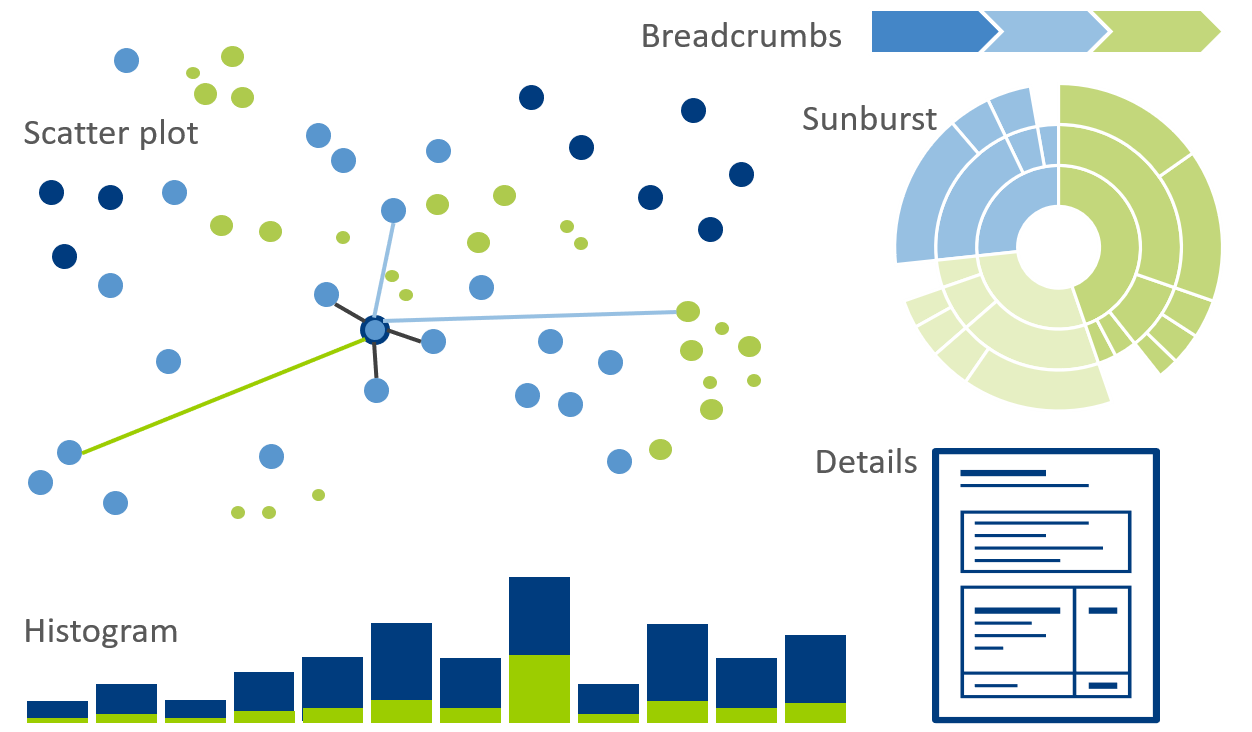
\includegraphics[width=\textwidth]{img/schematic}
\caption{A schematic representation of the visualization layout.}
\label{fig:schematic}
\end{figure}

\section{Ideation}
\label{sec:ideation}

In this section we justify the decisions that led to the creation of the visualization concept.
We then discuss the first iteration of the concept and the changes it went through during the development.

\subsection{Dimensionality of the visualization space}
\label{subsec:dimensionality_of_visualization_space}

The dimensionality of the embeddings that we intend to visualize is much too high to be plotted as it is.
A lower-dimensional presentation of the data must first be obtained via a dimension reduction technique. 
For that, a choice between 2D- and 3D-representation has to be made.
The latter provides an advantage in the sense that one additional dimension of the data can be displayed.
However, this gain comes with trade-offs with regard to usability.

Nielsen \cite{Nielsen1998} discourages using 3D for user interfaces.
He argues that while navigation in a 3D space looks impressive for an observer, it requires more cognitive resources from the user.
First, current interaction techniques are not specifically adapted for a 3D space and are cumbersome.
Second, even if the user successfully masters the controls, they still have to pay extra attention to navigating the 3D view in addition to navigating the information space.
The perspective itself introduces some usability problems. 
For example, remote objects are often hidden by nearby objects or are too small to be readable.
Additionally, it might be difficult to estimate the exact depth of an object or the distance between objects.

The plausibility of this line of reasoning has to be tested empirically.
Westerman et al. \cite{Westerman2000}, Banchs \cite{Banchs2014} and Fabrikant \cite{Fabrikant2007} performed comparison studies of 2D vs. 3D with regard to information retrieval tasks. 

Westerman et al. evaluated searching for objects in semantic spaces with multiple options for the amount of variance explained by all dimensions together.
They found that performance was generally poorer in three-dimensional condition with comparable amount of variance to a two-dimensional condition.
Moreover, they suggest that three-dimensional interfaces ``incur greater cognitive costs because of the demands of a more complex semantic mapping, i.e. maintaining a more complex mental model of the information space''.

In works of both Banchs and Fabrikant, 3D interfaces received positive feedback and were the participants' preferred representation.
In Banchs' study, the participants reported that the 3D platform allowed faster search, when in fact task completion times were lower for the 2D platform.
Notably, a higher percentage of tasks was accomplished successfully using a 3D platform.
Nevertheless, Banchs' conclusions match Nielsen's reasoning, namely that 2D interfaces are currently still more familiar to users.
Banchs highlights the performance of the visualization as one of the significant limitations, which was also mentioned by the participants.
This limitation also applies to our work, since our goal is to enable exploration of thousands of documents.

A notable exception from mentioned negative aspects constitute applications with entertainment purposes or for rendering physical objects in their solid form, where using 3D is encouraged \cite{Nielsen1998}.
Moreover, all above-mentioned arguments only apply assuming a pseudo-3D representation on a conventional two-dimensional computer screen.
A \gls{vr} application would define its own interaction techniques that feel natural for a 3D space.
Immersive data visualization in such environment using a \gls{vr} headset has been researched, for example in \cite{djorgovski2018immersive} and \cite{Hadjar2018}. 
Moreover, using a \gls{vr} environment implies a technology stack that is better adapted to displaying complex geometry, for example large point clouds.
Unfortunately, the advantages of a ``true 3D'' approach are not utilizable on a standard desktop workstation without extra hardware.

Ultimately, gaining one additional spacial dimension for representation is not worth the increased inconvenience of navigating the information space.
Therefore, we decided upon a 2D representation for our prototype.

\subsection{Choice of a suitable visualization metaphor for hierarchical data}

Most of the patent metadata attributes are of relatively common data types like date, string or list of strings.
But there is one attribute with an uncommon type and that is the \gls{ipc} class (described in \autoref{subsubsec:ipc_classification}), or more specifically, a list of \gls{ipc} classes.
\gls{ipc} classes are hierarchical in nature, which necessitates a suitable visual metaphor.

The \textit{treemap} as shown in \autoref{fig:treemap} is a space-filling type of diagram that was proposed by Shneiderman \cite{Shneiderman1992} and has often been used to visualize hierarchical data.
It uses nested shapes, usually rectangles, to represent the parent-child relationship.
A parent rectangle's space is divided into child rectangles along an axis that changes with each nesting level.
Size and color of rectangles represent various attributes of hierarchy nodes.
In an interactive version of a treemap, the user can select a node to examine its children in detail.
The available space is then redistributed to a subset of the hierarchy with the chosen node as its top.

\begin{figure}[!]
\centering
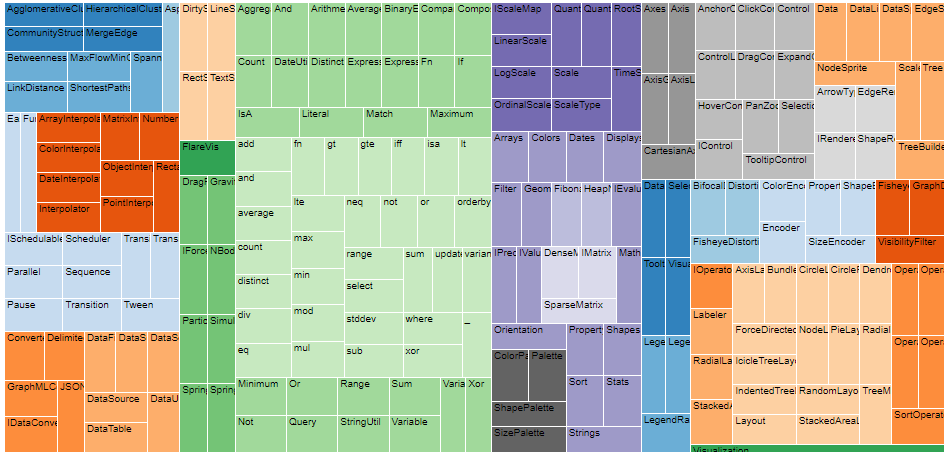
\includegraphics[width=0.7\textwidth]{img/treemap}
\caption{Treemap visualization of the class structure in a programming library Flare. Source: \cite{Takayuki2016}}
\label{fig:treemap}
\end{figure}

The \textit{sunburst} type of diagram was inspired by the treemap. 
It utilizes a radial layout in which child nodes are not contained in the parent nodes, but expand outwards from the circle center.
Size (angle) and color of the radial sectors can, just as with a treemap, represent chosen attributes of nodes in a hierarchy.
One can also navigate within the hierarchy by choosing a node to serve as a starting point in the center.

\cite{Stasko2000} evaluated treemap and sunburst in their study.
Their conclusion was that the sunburst ``more frequently aided task performance, both in correctness and in time, particularly so for larger hierarchies. The explicit portrayal of structure appeared to be a primary contributor to this benefit.''
Supported by this finding, we initially chose to use a sunburst for a fairly large hierarchy that is the \gls{ipc} classification.
Later, an idea emerged that the attributes represented by sunburst do not necessarily have to be of a hierarchical nature.
It is possible to ``stack'' multiple categorical attributes, for example country and assignee, to produce subgroups/child nodes which are represented in a sunburst.
Moreover, it is also possible to combine categorical and hierarchical attributes to show, for example, a distribution of \gls{ipc} classes per country.
In our visualization concept, we evaluate the feasibility of using metadata attributes of various types in a sunburst diagram.

\subsection{Initial concept and its evolution}
\label{subsec:initial_concept}

The initial concept was inspired by a demonstration of coordinated views showing mock data by \cite{Johnson2018}.
This demonstration implemented brushing and linking (see \autoref{subsubsec:brushing_and_linking} for more on brushing and linking).
The demonstration consists of a scatter plot on the left, a histogram on the right and an additional representation of a time axis at the bottom (see \autoref{fig:idea}).

\begin{figure}[!]
\centering
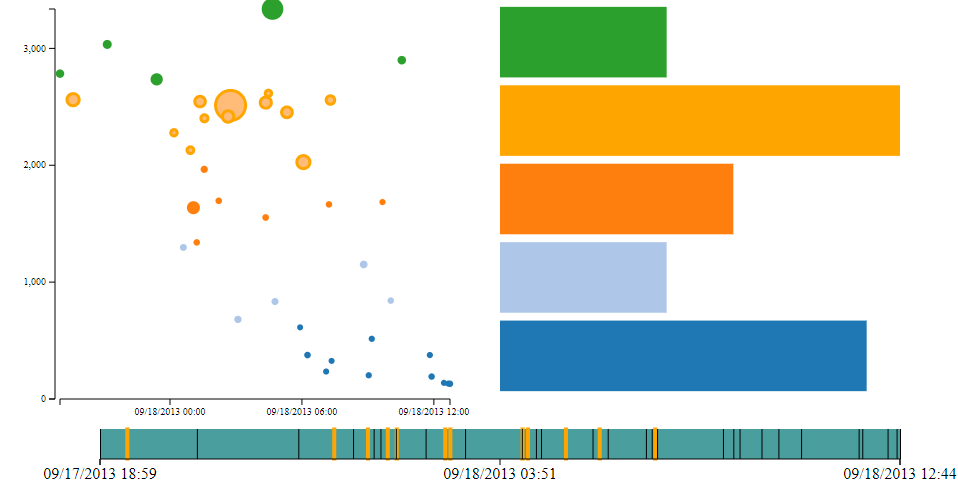
\includegraphics[width=\textwidth]{img/idea}
\caption{Demonstration of coordinated views that served as an inspiration for our concept. Image source and demo: \cite{Johnson2018}}
\label{fig:idea}
\end{figure}

The Y-axis of the scatter plot corresponds to a numerical dimension in the mock dataset, while the X-axis represents timestamps of data points.
The histogram splits the values of the numerical dimension into five bins.
The element at the bottom of the demo is essentially a \textit{rug plot}, i. e. it denotes the X-positions of data points by tick marks that look similar to tassels on a rug.
A classic example of a rug plot can be seen in \autoref{fig:rug_plot}.

\begin{figure}[!]
\centering
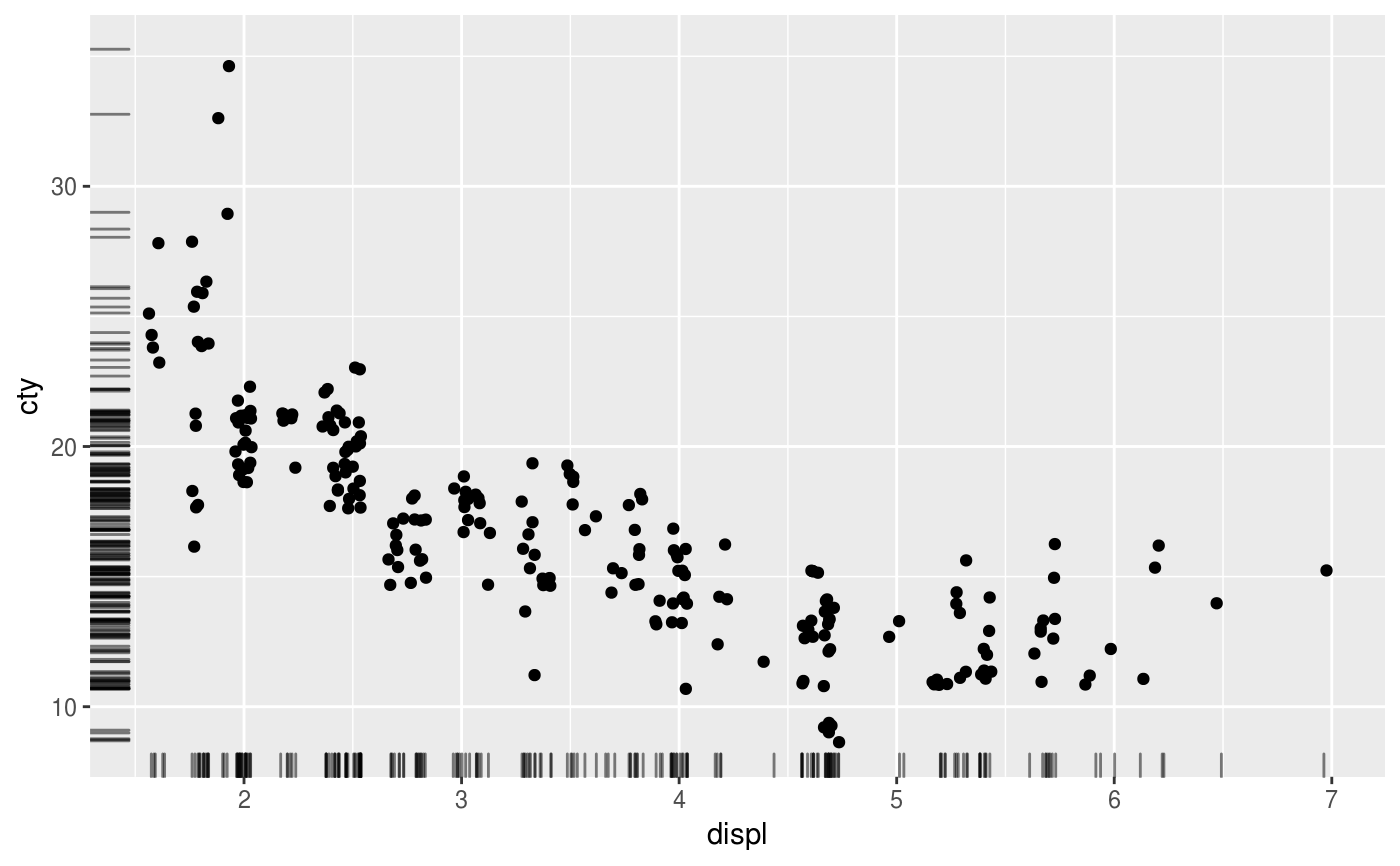
\includegraphics[width=\textwidth]{img/rug_plot}
\caption{A scatter plot is augmented with a rug plot. The rug plot shows distribution of the data points with regard to X and Y coordinates. Image source: \cite{rug}}
\label{fig:rug_plot}
\end{figure}

Rug plots are used to illustrate the distribution of a variable along the axes, in this case the time axis.
Usually, a rug plot is drawn as a part of the original plot (scatter plot, line plot, histogram, etc.), but in this instance it has been separated from the corresponding scatter plot.
The main purpose of the element is to enable selection of the data by brushing and linking, which is why we and the author refer to it as the \textit{brush element}.
The histogram values are recomputed in accordance with the updated selection.
Moreover, when the mouse is hovering over the histogram bins, corresponding data points are highlighted both in the scatter plot and in the brush element.

The first iteration of our visualization concept  (see \autoref{fig:sketch}) was built on ideas borrowed from the above-mentioned demonstration by \cite{Johnson2018}.

\begin{sidewaysfigure}
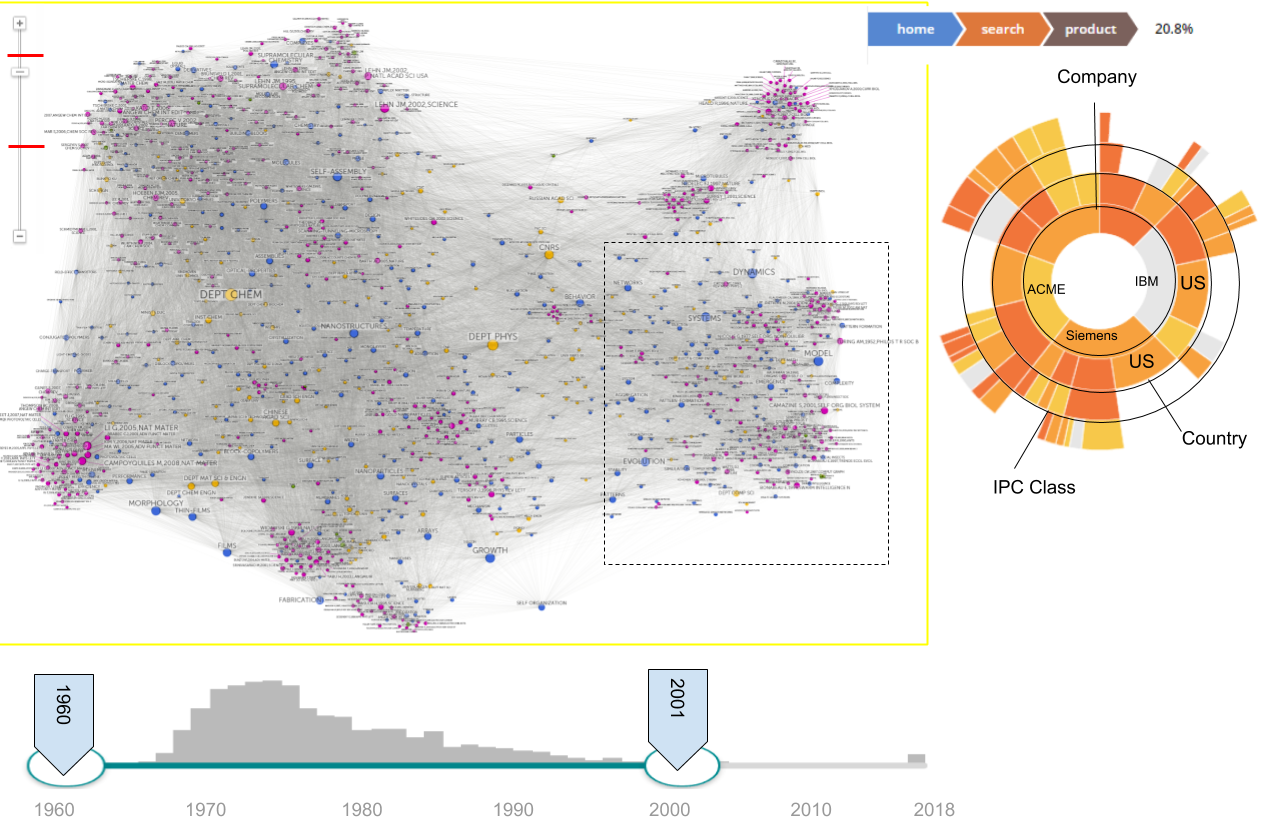
\includegraphics[width=\textwidth]{img/Visualization_mockup}
\caption{The first iteration of the visualization concept. Source of the graph picture: \cite{Latour2012}, source of the sunburst picture: \cite{Ribecca2019}.}
\label{fig:sketch}
\end{sidewaysfigure}

Firstly, it was the idea of a main area that contains data points and is influenced by controls on the edge of the display.
Displaying distribution of patent applications over time and the ability to select a time interval we consider especially useful for the patent landscaping use case.
Therefore, we decided to implement the same linking and brushing functionality, yet considering the size of the data, a histogram with yearly bins was judged more fitting to show the distribution over time.

Secondly, inspired by the ideas from \cite{Johnson2018} and \cite{Wittenburg2015}, our UI concept was designed to show a distribution of the dimensions of the data.
In our case those attributes are mostly categorical, and \gls{ipc} classes are also hierarchical in nature.
The wish to display multiple dimensions of the metadata resulted in our choice of a sunburst chart in the place of a histogram in the original demonstration.
This decision was partly motivated by Wittenburg et al. \cite{Wittenburg2015}, who make extensive use of metadata in their faceted visualization (see \autoref{fig:wittenburg}).
They show the assignee, country and application year as a vertical stack of blocks where the width of a block corresponds to the number of patents with the corresponding attribute value. 
Unfortunately, their approach results in a cluttered view and therefore lacks visual scalability.
We address the scalability problem via interactivity, i. e. through the fact that it is possible to change levels of a sunburst chart 1) through navigating up and down the hierarchy of attributes and 2) by choice of different sets of metadata attributes to be charted.
For more details on our implementation of the sunburst chart see \autoref{subsec:sunburst_and_breadcrumbs}.

The main area of our visualization was initially conceived as a fully connected graph.
Similarities between each pair of documents were supposed to correspond to the attraction forces in the force-directed graph layout.
When a part of the dataset would be eliminated through filtering, the corresponding graph nodes would disappear and the whole layout would rearrange itself.
Effectively, the process would amount to computing and then dynamically updating a \gls{tsne} representation of the dataset. 
An interactive demonstration of such a layout is presented in \cite{Strayer2018}.
While it would certainly be of value to cluster subsets of the data dynamically depending on the selection, performance considerations outweigh the benefits.
Therefore, a scatter plot with static positions of data points was chosen as a viable alternative.

Initially, the concept included no standalone detail view.
Instead, the idea was to display some tooltip elements directly above the currently chosen patent and above patents related to it.
Type and amount of the information presented in the tooltips were supposed to change depending on current selection and zoom level according to the principle of \textit{semantic zooming}.
Upon further consideration it became clear that such tooltips would cover a significant portion of the scatter plot and would therefore render it unusable.
The decision was made to place the detailed patent information to the available space in the lower-right corner.

The zoom control in the upper-left corner is an idea borrowed from various interactive map interfaces.
The red markings were supposed to show boundaries between different detail levels of hierarchical clustering.
Ultimately, we implemented different visual indications that sufficiently support the feeling of ``moving into'' the landscape and back, so this part of the initial concept was omitted.
Other elements were utilized in the prototype without changing much.

\section{Data processing}
\label{sec:pipeline}

Before a dataset can be displayed in a visualization, it has to be processed in a preparatory step.
\autoref{fig:pipeline_single} and \autoref{fig:pipeline_all} present an overview of the processing pipeline which is necessary to produce data for the visualization.
In this section, we give a brief overview of the steps, which are covered in more detail in \autoref{sec:implementation_of_data_processing}.

\begin{figure}[!]
\centering
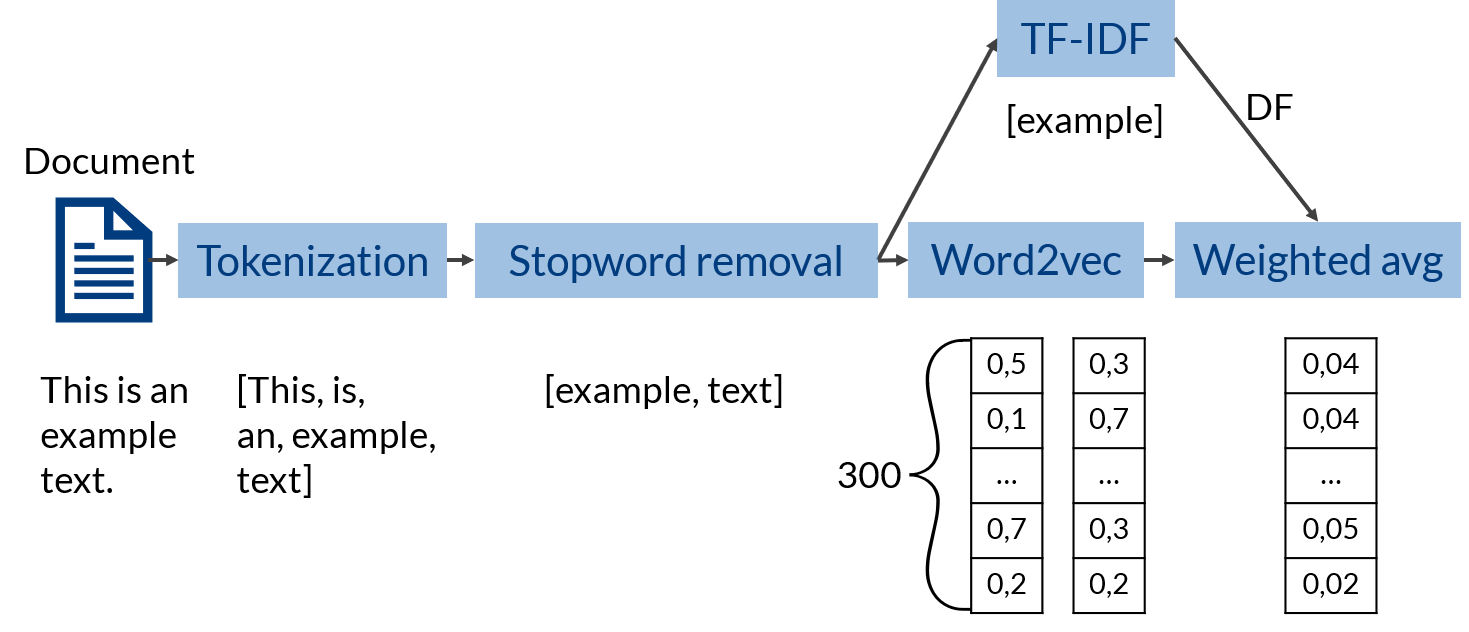
\includegraphics[width=0.9\textwidth]{img/pipeline_single}
\caption{Pipeline of processing steps for a single patent document}
\label{fig:pipeline_single}
\end{figure}

First, each patent needs to be processed individually (see \autoref{fig:pipeline_single}).
This starts with splitting the textual part into separate words and removing stopwords.
Stopwords include general grammar-related words such as ``is'', but also patent-specific vocabulary such as ``embodiment''.
Then, for each word a 300-dimensional embedding is retrieved from the word2vec model explained in more detail in \autoref{subsec:data_source}.
A vector representing the whole document is composed by aggregating the word vectors as a weighed average.
Each word is weighted with its IDF.
Our purpose is to make semantic similarities and differences tangible, but numerical document vectors do not provide an explanation of why any pair of documents are close or distant. 
Therefore, TF-IDF is also used to extract relevant key terms per patent.

\begin{figure}[!]
\centering
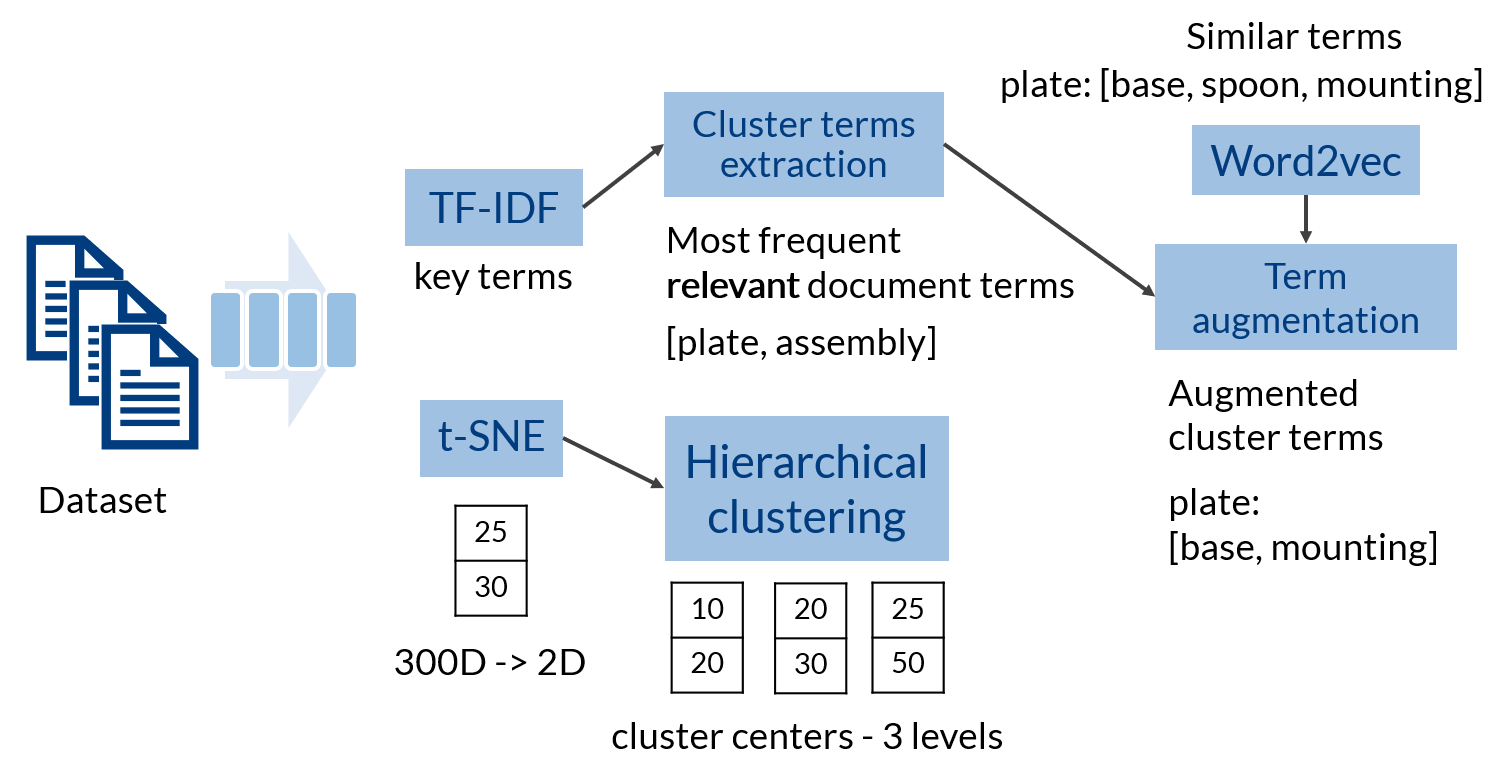
\includegraphics[width=0.9\textwidth]{img/pipeline_all}
\caption{Continuation of the pipeline after all individual patents have been processed}
\label{fig:pipeline_all}
\end{figure}

Second, after all document vectors and document key terms are computed, the processing on the dataset as a whole can begin (see \autoref{fig:pipeline_all}).
300-dimensional document vectors are reduced to two dimensions with \gls{tsne} to fit the visualization space.
This enables hierarchical clustering, which splits the dataset into a number of clusters on three detail levels, resulting in large, medium and small clusters.
It is crucial for user's understanding to know what common semantic characteristics the grouped patents share.
To cover that, we extract the key terms per cluster.
We take most relevant terms per document and count them across all patents within a cluster. 
The terms with most occurrences are assigned to the cluster to explain its thematic focus.

To aid the understanding of cluster key terms, for each single-word term we retrieve similar words from the above-mentioned word2vec model.
We then check whether those similar words occur in more than 10\% of the patents in the cluster.
If that is the case, the word is added to the list of augmenting terms for the given key term.
For example, if we try to augment the term \textit{plate}, the word2vec model might retrieve \textit{base, spoon, mounting} as similar words because they often appear in similar contexts with \textit{plate}.
Assuming the dataset is not about cutlery, \textit{spoon} does not appear in many patents, but \textit{base} and \textit{mounting} might. 
Therefore, \textit{base} and \textit{mounting} are the terms that provide context for the term \textit{plate} in the given cluster.

Herewith the processing of the textual part of the patent dataset is complete.
As for metadata, some of the attributes can be used in the visualization as is, while others require special processing (see \autoref{subsec:data_preprocessing} ``Parsing of metadata attributes'' and \autoref{subsec:hierarchies}).
We elaborate on the processing of both textual and metadata parts of a patent dataset in \autoref{sec:implementation_of_data_processing}.


%% LaTeX2e class for student theses
%% sections/content.tex
%% 
%% Karlsruhe Institute of Technology
%% Institute for Program Structures and Data Organization
%% Chair for Software Design and Quality (SDQ)
%%
%% Dr.-Ing. Erik Burger
%% burger@kit.edu
%%
%% Version 1.3.3, 2018-04-17

\chapter{Implementation}
\label{ch:implementation}

After having defined the concept for our approach as described in the previous chapter, we created a proof-of-concept prototype to evaluate our approach.
In this chapter, we describe both the visual part of the implementation and the behind-the-scenes processing which serves to prepare the data to be visualized.

The code of the implementation can be found at \url{https://github.com/gingergenius/patent-embedding-visualization}.

\section{Implementation of the data processing}
\label{sec:implementation_of_data_processing}

In this section we describe what data source we use.
We then justify our choice of programming languages and tools.
Finally, we elaborate on the data processing pipeline described briefly in \autoref{sec:pipeline}.

\subsection{Data source}
\label{subsec:data_source}

Google Patents Public Datasets \cite{IanWetherbee2017} is a data source available for public use on Google’s BigQuery platform. 
It contains full-text patent publications for the US and bibliographic data (abstract + metadata) for patents filed in the rest of the world (see \autoref{subsubsec:structure_of_a_patent_document} for the description of data fields per patent).
The database has about 100 million patent document records and is updated quarterly. 
While a quick examination of a sample of the data revealed some format errors, probably resulting from optical recognition, most of the text is readable.
This data source is therefore sufficient for a quality analysis.

We extracted four separate datasets about different technology domains from Google Patent Public Datasets:
\begin{itemize}
	\item \textit{Hair dryer} contains approximately 250 patents. It was included in the codebase from \cite{Abood2018a} and consists purely of patent applications from the US. Because of relatively small size of this dataset, separate thematic areas within it are not clearly distinguishable.
	\item \textit{Video codec} contains about 1600 patents. It was also included in the codebase from \cite{Abood2018a} and consists purely of patent applications from the US. This dataset consists overwhelmingly of patent families of different sizes. Because of that, it is suitable for evaluating how well the family similarities are handled by the semantic embeddings. However, because of our unfamiliarity with the topic of video encoding, an alternative dataset was necessary for the evaluation.
	\item \textit{3D printer} with roughly 1000 patents was produced by us using a query adapted from an existing patent landscaping report \cite{report_3d}. The full text of the query can be seen in \autoref{sec:3d_printer_query}. The dataset consists of both US and non-US patents. Non-US patents have only abstract text available while US patents have all textual fields available, of which we use the abstract and claims. We wished, however, to exclude effects resulting from different text lengths, but still make a considerable number of patents available for exploration. Consequently, we additionally prepared the contact lens dataset.
	\item \textit{Contact lens} consists of ca. 2600 patents and was based on a query adapted from an existing patent landscaping report \cite{report_lenses}. The full text of the query can be found in \autoref{sec:contact_lens_query}. We restricted this dataset to US-only patents so that we would be able to work with both the abstract and claims for the whole dataset. The contact lens dataset contains a variety of topics and is large enough for interesting exploration tasks. This is why we chose it for our evaluation.
\end{itemize}

Additionally, FIZ Karlsruhe kindly provided one more dataset extracted from the \gls{wipo} database on the topic of diesel engines (ca. 4500 patents).
The patents in it had both abstract and claims available, but no citation or family information.
Moreover, multiple languages were present in the text and everything beside English had to be filtered out.
This dataset was necessary to check how the approach performs on large data.
Unfortunately, it could not be used for the evaluation with experts because of the missing metadata attributes.

Many existing pretrained models for word embeddings are based on general vocabulary. 
Language and especially vocabulary in patent documents deviate significantly from general speech, which must be taken into account. 
Abood et. al \cite{Abood2018a} provide a word2vec model trained on 5.9 million patent documents. 
It contains a 300-dimensional embedding for each of 110239 words in its vocabulary.  
We make use of this model for our semantic analysis to compute document embeddings.

\subsection{Choice of technology}
\label{subsec:choice_of_technology}

Python \cite{python} is chosen as the programming language for preparing the data for visualization. 
It is an extremely widespread language in the field of machine learning with a great number of libraries available.
Of those libraries, Tensorflow \cite{tensorflow} in combination with Keras as a high-level \gls{api} \cite{keras} is a state-of-the-art library for neural networks. 
In fact, \cite{Abood2018a} used them in their approach for data preprocessing and for creating the word2vec model we use.
We based our approach on their codebase, so Tensorflow and Keras were also inherited by us.
Other widely used Python libraries we take advantage of are Numpy \cite{numpy} and SciPy \cite{scipy} for scientific computing and scikit-learn for machine learning.
Finally, JupyterLab \cite{jupyterlab} with an IPython \cite{ipython} kernel is selected as the development environment of choice because of ease of quick prototyping.

For the interactive visualization itself, information visualization frameworks such as Axiis \cite{axiis}, Bokeh  \cite{bokeh}, D3.js \cite{Bostock2019}, Altair \cite{altair}  and several others were considered. 
For the given problem, creating both custom user interaction techniques and custom visualization layouts consisting of new forms of charts is required. 
Unfortunately, most visualization frameworks do not support this.
Instead, they restrict the developer's alternatives to pre-determined chart types.
Coordinated interactions between views are either not supported or very limited.
Consequently, D3.js is chosen as the visualization framework with most flexibility.
It requires a hands-on, low-level approach to programming, where the developer has to manually define SVG shapes and bind their attributes such as position or color to the data.
However, this is exactly why D3.js provides the necessary level of control for the implementation of our prototype.

\subsection{Data preprocessing}
\label{subsec:data_preprocessing}

In \autoref{subsec:data_source}, we mentioned multiple datasets that were prepared for the visualization in the course of this work and the queries used to produce them.
In this section, we describe the preprocessing steps that are executed for each patent document within a retrieved dataset.

The diesel engine dataset was, unlike the others, not derived from Google Patents Public Datasets, so it required some minor additions to the pipeline.
The data structure was slightly different and therefore had to be transformed for compatibility.
Moreover, the patent texts had to be cleaned as there were some \gls{xml} tags present that we removed.
Additionally, the diesel engine dataset included a non-negligible amount of text in French and German within the patent claims. 
To filter out non-English text, we split the text into sentences and detected their language using the Python library langid \cite{Lui2012}.
This language detection tool utilizes a multinomial naive Bayes classifier trained on n-grams to reliably produce a robust result independently of domain and text length \cite{Lui2011}.

The interviews with the patent experts indicated that title, abstract and claims are the most valuable textual parts of a patent document for understanding the described invention.
Other textual parts, such as background art or description of figures, do not contribute significantly to the essence of the invention.
Therefore, for all further steps we concatenate the patent's title, abstract and, when available, its claims.
This way, we maximize the length of relevant textual content taken into account.
We do not consider the three above-mentioned textual fields separately for sake of simplicity.
However, for future work it might be worth examining how different textual parts of the same document compare to each other when semantic methods are applied to them separately.

\paragraph{Tokenization}~\\
The proper preprocessing starts with \textit{tokenization}, which means splitting the text into tokens.
Tokens in our case are not characters or sentences but words since we use word embeddings from a pre-trained word2vec model.
We use a \verb|Tokenizer| class from Keras which replaces all punctuation except the apostrophe character with spaces.
It then translates the whole text to lowercase and splits the text into words divided by spaces.
The last step is replacing the numbers that occur separately or as parts of a word with a \verb|_NUMBER_| token. 

\paragraph{Stopword removal}~\\
After we have successfully tokenized the data, the next step in the pipeline is the stopword removal to increase the amount of meaningful information per document.
We use two stopword lists: one is a general list of English stopwords from Natural Language Toolkit \cite{bird2009natural} and the other one is a patent-specific list kindly provided by FIZ Karlsruhe.
The latter list includes words like ``comprised'', ``abovedescribed' and ``obtained'' which often appear in patent texts and do not contribute to the meaning.
Words shorter than 3 characters or longer than 50 characters are eliminated as well.
Finally, when the number of meaningful words per patent becomes clear, we remove all patent documents that contain less than 30 words.
The amount of the remaining text at this stage varies between the datasets, but in all cases it followed a left-skewed distribution with a mode of approximately 250 words and an average of 500 up to 1000 words.
Distributions for diesel engine and contact lens can be found in \autoref{fig:text_length_distributions}.
 
\paragraph{Parsing of metadata attributes}~\\
This step is independent of the processing of textual content, but instead prepares the metadata attributes for visualization.
Metadata attributes such as references, assignees and \gls{ipc} classes are included in the data as a string made up of comma-separated values, so we split the list to get each separate value.
For \gls{ipc} classes, we compute a list of unique codes for all levels of the \gls{ipc} hierarchy per document (see \autoref{table:ipc_classes_structure} for description of levels).

The assignee names present a challenge with regard to the data quality.
Institutions' legal names are written out in a very inconsistent way throughout the data.
There are often multiple variants with parts of the name which are abbreviated in some cases but not in others.
Different branches or subsidiaries of the same company are also often present.
Lastly, there are errors and misspellings as well, partly as a result of \gls{ocr} artifacts.
This last point applies to assignee names signifying private persons as well as companies.

We would like to be able to reliably group patents by their assignees.
For this, we merge similar assignee names with \textit{fuzzy string matching}, which is a technique of finding strings that are approximately the same.
We use the Python library \verb|FuzzyWuzzy| \cite{Cohen2011}, which is based on Levenshtein distance between two sequences of characters.
The Levenshtein distance is a measure of similarity composed of the number of character deletions, insertions or substitutions required to transform one string into another \cite{levenshtein}.
The value returned by the library is not the absolute distance but a similarity percentage that takes string length into account.
We use a simple similarity threshold of 88\% to determine which assignees to combine into one entry.
The threshold value was chosen empirically to provide sufficiently good results.
Fuzzy string matching allows us to reduce the number of unique assignees in the dataset by 10-15\%.
However, false positives (match detected where none exists) and false negatives (existing match not detected) could not be completely excluded from among the matches.

\subsection{Sunburst hierarchies}
\label{subsec:hierarchies}

As we would like to use the sunburst control for arbitrary combinations of metadata attributes, corresponding hierarchical aggregations need to be computed.
For that, we consider \gls{ipc} class, country, assignee by themselves and also all possible permutations (orderings) of those attributes of size two.
We do not consider stacking all three attributes as sunburst levels because of space restrictions and because the groups after the third division would become very small.
However, it would only be effective for larger datasets and documents with multiple non-hierarchical metadata attributes.

For metadata attributes, we distinguish between a single value per document (e. g. country), a list of values per document (e. g. assignee) and a hierarchical code such as an \gls{ipc} code or a list of such codes.
This allows us to adjust how the aggregation is computed depending on the type of the attribute.
For \textit{value attributes}, we can just group all documents by their unique values of the corresponding attribute.
For \textit{list attributes}, a single document can be referenced in multiple hierarchy nodes, so it should be counted multiple times.
\textit{Code attributes} are essentially multiple list attributes in a certain order (section, class, subclass, group, subgroup) with one extra condition: a subclass from one \gls{ipc} code (for example, N04N) can only count as a child of its own class (N04) and not some other class (B02).

As mentioned in \autoref{subsubsec:sunburst}, because patents simultaneously belong to multiple nodes, a total number of patents in the hierarchy may exceed the size of the dataset.
In this case, the values of all nodes are normalized so that they yield 100\% when combined.
The normalization starts from the shallowest hierarchy level and then goes into the depth.

\subsection{Key term extraction}
\label{subsec:term_extraction}

We extract relevant key terms per document so that the user can get a first impression of the content of a document with just a quick glance.
For this extraction we use \gls{tf-idf} which is a widely used weighting technique to determine most important words or phrases in a corpus.
Essentially, the more often a phrase occurs in a document, the most important it is for this document (\gls{tf}).
At the same time, the more often the same phrase occurs throughout the whole document corpus, the less explanatory power it has (\gls{idf}).

For our data, unigrams (single words) and bigrams (two-word phrases) produce most meaningful results.
To exclude extremely rare terms and spelling mistakes, only phrases that occur in more than ten documents are considered for their relevancy.
Additionally, we also explicitly exclude terms appearing in over 20\% of the corpus from consideration because they are unlikely to result in an information gain.
For each patent, we save a list of ten terms that were most highly ranked by \gls{tf-idf} for visualization.

\subsection{Embeddings}
\label{subsec:embeddings}

\paragraph{Document vectors}~\\
The purpose of this stage is to produce a representation of a document based on the words it consists of.
The input of this step is a sanitized list of words per patent, which is a result of the tokenization and stopword filtering operations described in \autoref{subsec:data_preprocessing}.
We compute each document embedding as a weighed average of the embeddings of words the document contains.
300-dimensional word embeddings are retrieved from the pre-trained word2vec model provided by \cite{Abood2018a}.
The weighting factor for each word is its \gls{idf}, which at this point had already been computed as described in \autoref{subsec:term_extraction}.
Adjusting the weight of a word by its frequency in the corpus takes the varying importance of separate words into consideration and therefore helps capture themes in the dataset in a better way.
Weighting with \gls{idf} has been successfully used for computing semantic similarity \cite{Zhao2015} \cite{NAGOUDI2018}, \cite{Arora2017} and for sentiment analysis \cite{Correa2017}.
In our case, we found that compared to non-weighted word averages, weighted word vectors result in a clearer separation of clusters after dimension reduction compared to non-weighted word vectors.
The documents were more likely to gather into dense groups instead of being distributed uniformly.
A comparison of weighted and non-weighted word averages can be seen in \autoref{fig:weighted_vs_average_diesel} and \autoref{fig:weighted_vs_average_contact_lens}.

\begin{figure}[!]
    \centering
    \subfigure[Non-weighted average]
    {
        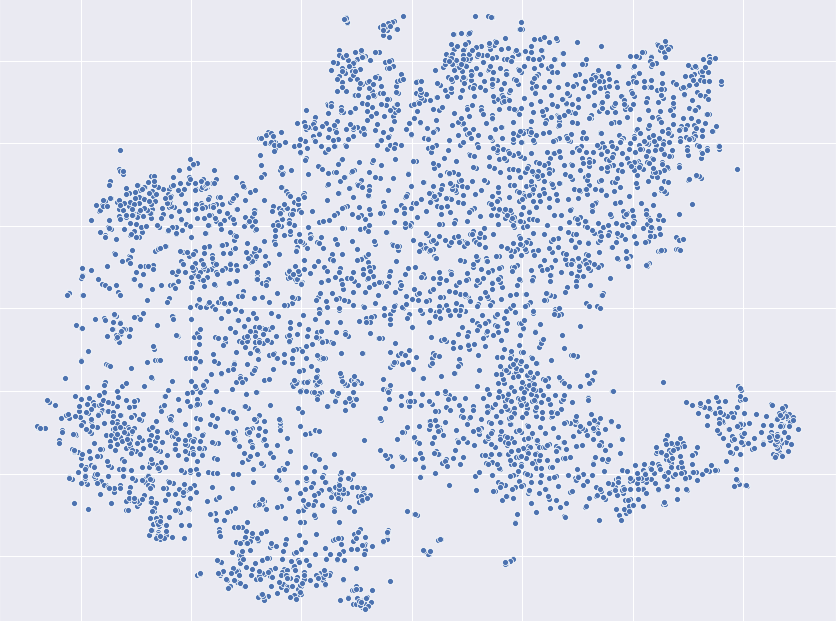
\includegraphics[width=0.95\textwidth]{img/diesel_avg}
    }\\
    \subfigure[Weighted average]
    {
        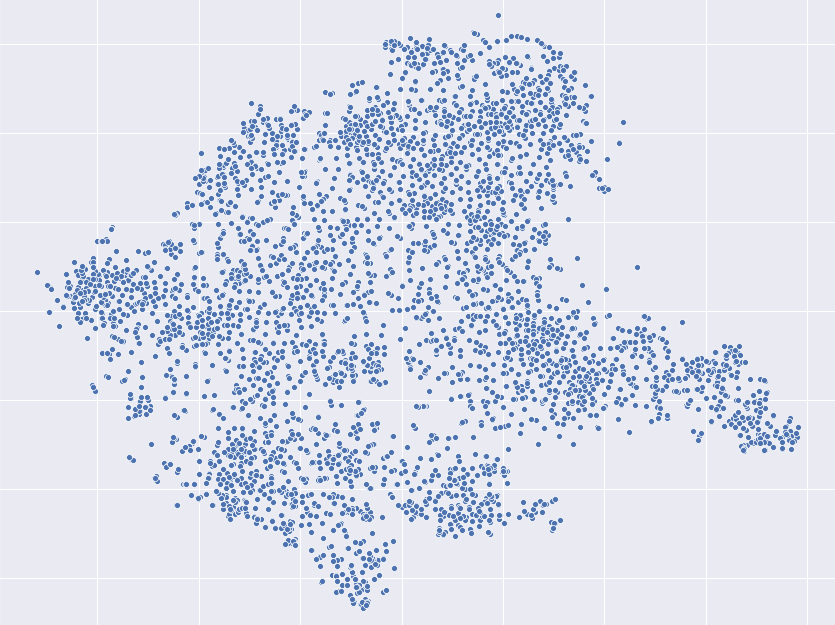
\includegraphics[width=0.95\textwidth]{img/diesel_weighted}
    }
    \caption{A comparison of document vectors computed with and without \gls{idf} weighting. Diesel engine dataset.}
    \label{fig:weighted_vs_average_diesel}
\end{figure}

\paragraph{Dimension reduction}~\\
Points in a very high-dimensional space are not suitable for an understandable visualization.
For the purposes of visualization we need to transform document vectors into a two-dimensional space so that any patterns in the data become recognizable.

We compared multiple dimension reduction techniques such as metric and non-metric \gls{mds} \cite{OConnell2006}, Isomap \cite{Tenenbaum2000}, \gls{pca} \cite{hotelling1933analysis}, \gls{umap} \cite{McInnes2018} and \gls{tsne} (see \autoref{subsubsec:tsne}).
In the interviews, patent experts emphasized that patents from the same family possess a great degree of semantic similarity and one should expect them to be placed closely to each other (see \autoref{subsec:implications}).
Handling patent families correctly is a minimum requirement for a suitable dimension reduction technique.
For this reason, the comparison was conducted on the video codec dataset since it chiefly consists of patent families of different sizes.

Among the tested dimension reduction techniques, \gls{tsne} was the only one in which families were clearly identifiable and separated from their surroundings.
Figure \autoref{fig:tsne_video_codec} shows numerous ``clumps'' of closely situated points.
Further inspection showed that they mostly belonged to the same family, even when the family information present in the dataset was incomplete and did not explicitly list a connection.
In the majority of other cases, the patents within the groups belonged to the same assignee, dealt with the same invention and were therefore textually very similar (see Figure \autoref{fig:tsne_video_codec_double}).
When tested with other datasets, \gls{tsne} resulted in easily identifiable accumulations of points distinctly separated from each other by empty areas.
Other techniques were apt to clump the points into one big area or distribute them uniformly without defined groups.
Large sparse zones consisting purely of apparent outliers were also likely to appear.
For comparison, see \autoref{fig:other_dimension_reduction} for the results from other dimension reduction methods.

\begin{figure}[!]
    \centering
    \subfigure[The result of the dimension reduction by \gls{tsne}. The points are plotted in the same color and size to make close groups visible]
    {
        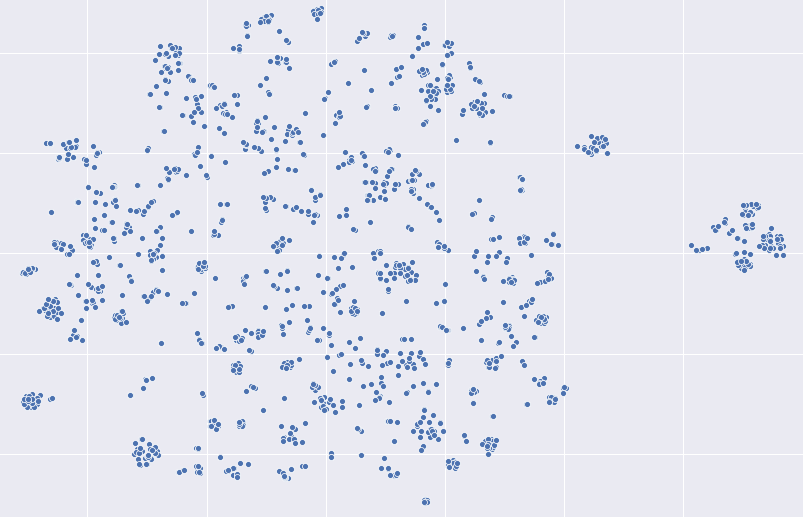
\includegraphics[width=\textwidth]{img/tsne_video_codec}
        \label{fig:tsne_video_codec}
    }\\
    \subfigure[Same coordinates as above, displayed in the interactive prototype. The patents from the same assignee are drawn in the same color, which shows that groups constitute patent families]
    {
        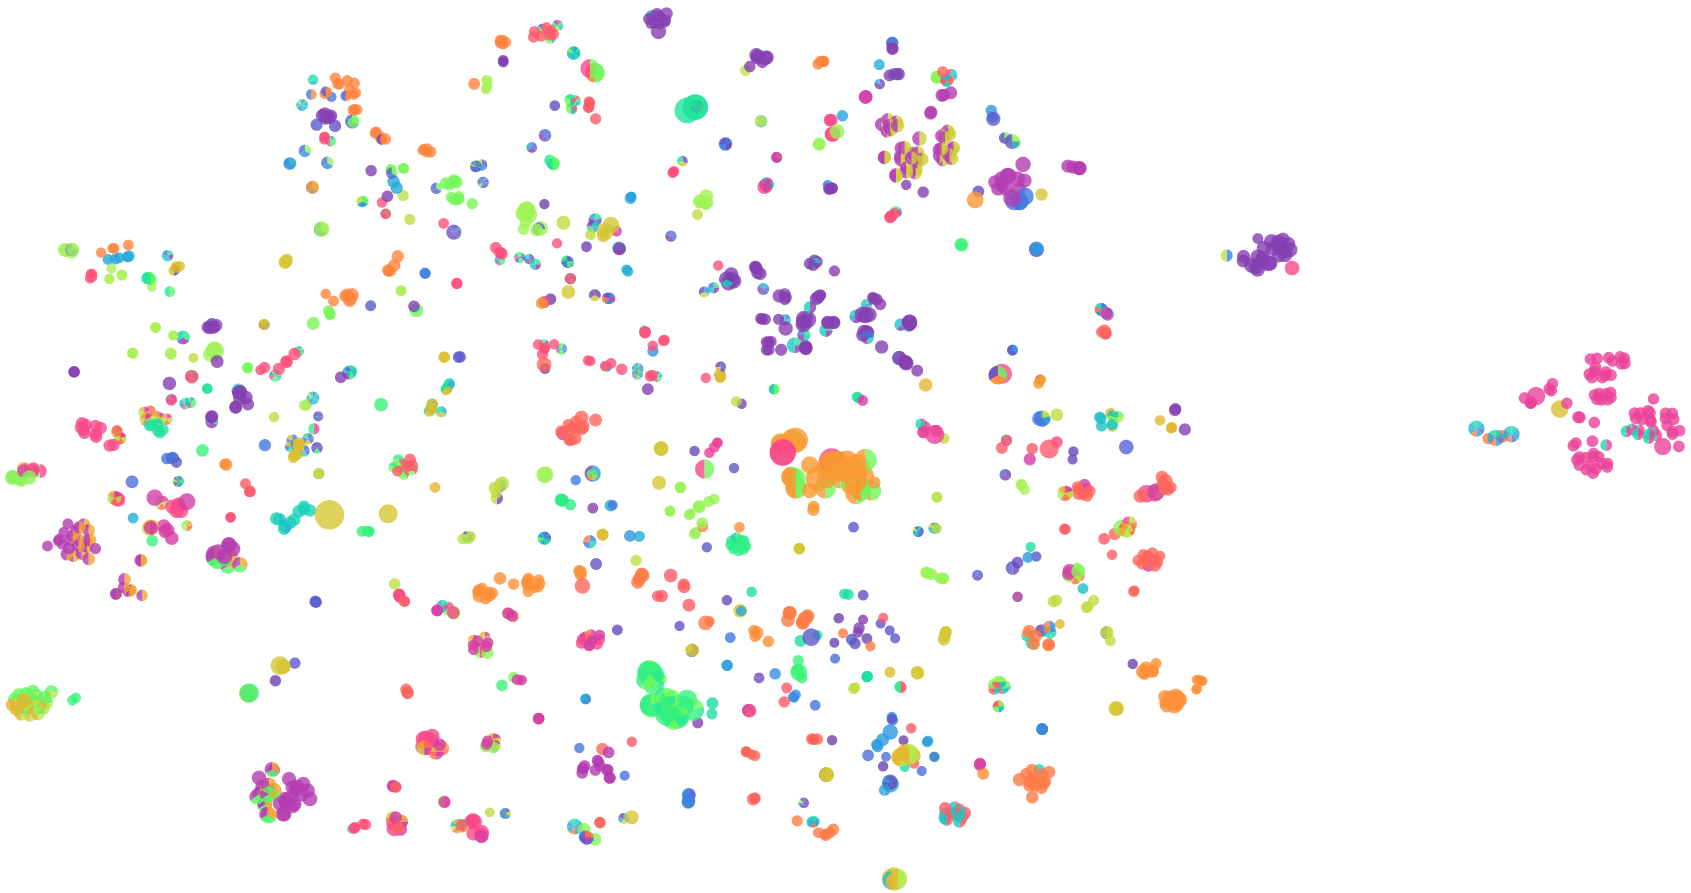
\includegraphics[width=\textwidth]{img/tsne_video_codec_assignees}
        \label{fig:tsne_video_codec_assignees}
    }
    \caption{The result of dimension reduction by t-SNE on the video codec dataset.}
    \label{fig:tsne_video_codec_double}
\end{figure}

As \gls{tsne} tries to retain distances from the high-dimensional space in the lower-dimensional representation (see \autoref{subsubsec:tsne} for details), a suitable \textit{distance metric} has to be used.
Distances in high-dimensional spaces behave in a non-intuitive way and currently there is no consensus on the ``best'' metric for all possible applications.
We experimented with multiple distance metrics such as euclidean distance, cosine similarity and manhattan distance.
The local structure of the data seemed stable independently of the used metric, only the relative placement of larger groups changed.
Ultimately, we settled on \textit{cosine similarity}, which is widely used in \gls{nlp} applications.
For two vectors A and B, cosine similarity is measured as the cosine of the angle between them.
It can be derived easily using a dot product as shown in \autoref{eq:cosine}.

\begin{equation} \label{eq:cosine}
\mathbf{A} \cdot \mathbf{B}=\|\mathbf{A}\|\|\mathbf{B}\| \cos \theta
\end{equation}

As a result of this stage, 300-dimensional document vectors have been transformed into two dimensions for visualization using \gls{tsne} with cosine similarity as a distance metric.

\subsection{Hierarchical clustering}
\label{subsec:hierarchical_clustering}

At this step we have 2D coordinates of all patents, but it is not immediately clear to the user why they are placed in a certain way. 
To explain the semantic similarities within groups at multiple levels of detail, we use agglomerative (bottom-up) \textit{hierarchical clustering}.
Essentially, is a process in which every data point is considered its own cluster at the beginning. 
Those singular clusters are then merged into their nearest clusters  one-by-one, and in the following iterations, clusters join the adjacent clusters until the whole dataset is joined into one single cluster.
The changes are tracked throughout the algorithm within a \textit{distance matrix}, in which pairwise distances between any two clusters are stored.
The process constructs a tree called \textit{dendrogram} which reflects the structure present in the distance matrix.

An example dendrogram is shown in \autoref{fig:example_dendrogram}.
Points E and F are the nearest pair of points in the dataset, so they are combined to a cluster EF on the first iteration of the algorithm.
The same thing happens to A and B on the second iteration.
Point D and subsequently point C join cluster EF and finally, cluster AB and cluster CDEF are merged to create a root node of the hierarchy.
Since it is a tree structure, there is no single correct number of clusters in a hierarchical clustering.
After every merge one can decide to make a ``cut'' as shown by the orange line.
At this specific level of detail, the dataset is then divided into a number of clusters equal to the number of dendrogram lines the cut crosses.

\begin{figure}[!]
\centering
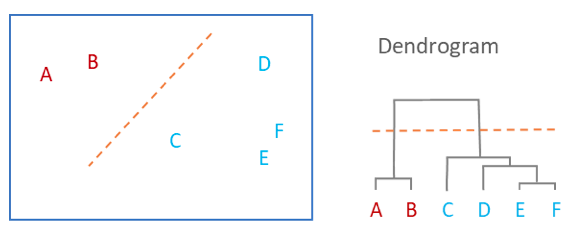
\includegraphics[width=0.7\textwidth]{img/example_dendrogram}
\caption{An example of dendrogram used in hierarchical clustering and its input data. Image source: \cite{Bock}}
\label{fig:example_dendrogram}
\end{figure}

A distance between any two points is clearly defined in a 2D space, but multiple definitions exist for distance between two clusters.
SciPy's \verb|linkage| method, which we used as an implementation of the hierarchical clustering, offers various options for calculating the distance between two clusters:
\begin{itemize}
	\item \verb|single| (Nearest Point Algorithm) uses the minimal distance between points from different clusters
	\item \verb|complete| (Farthest Point Algorithm) uses the maximal distance between points from different clusters
	\item \verb|average| uses $d(u, v)=\sum_{i j} \frac{d(u[i], v[j])}{(|u| *|v|)}$ where $u$ and $v$ are the two clusters and |u| and |v| are their respective cardinalities
	\item \verb|weighted| uses $d(u, v)=(d i s t(s, v)+d i s t(t, v)) / 2$ where clusters $s$ and $t$ were previously combined to form $u$ and $v$ is the remaining cluster
\end{itemize}

To identify the best algorithm, we computed a Cophenetic Correlation Coefficient \cite{sokal} for all above-mentioned algorithms on all five of our datasets.
The coefficient compares (correlates) the actual pairwise distances of all data points to those implied by the hierarchical clustering. 
The closer the value is to 1, the better the clustering preserves the original distances. 
The method \verb|average| consistently produced higher values of Cophenetic Correlation Coefficient across the datasets, which made it our preferred method.

Besides clustering in 2D space after the dimension reduction, we experimented with clustering in the original 300-dimensional document space as well.
The resulting structures were not preserved well during the dimension reduction.
The clusters were not clearly divided, which means it was impossible to draw a clear boundary between clusters.
This led to problems with placing cluster labels as described in \autoref{subsubsec:clusters}.
We therefore prefer clustering data in the same space where it is visualized.
This is due to a compromise that has to be made between representing the structures in the original high-dimensional space accurately and keeping the end result sufficiently simple for human cognition and therefore interpretable.

An example of a resulting dendrogram is shown in \autoref{fig:dendrogram_contact_lens}.
We manually chose three levels of detail for each dataset according to consistent principles.
We refer to the levels of detail in terms of \textit{large}, \textit{medium} and \textit{small} clusters.
\begin{itemize}
\item The number of large clusters should be between 3 and 7 depending on the structure of the dataset. 
At this level the most general topics in the dataset should be visible.
\item The number of medium clusters should be between 10 and 20, so that every large cluster is divided into approximately 3 to 4 smaller topics.
\item The number of small clusters should be between 40 and 70, so that every medium cluster is divided into 3 to 4 parts.
This finest level of detail is aimed at summing up patent families and very closely related inventions.
\end{itemize}
An example separation of a dataset into large clusters is presented in \autoref{fig:contact_lens_large}.

\begin{figure}[!]
\centering
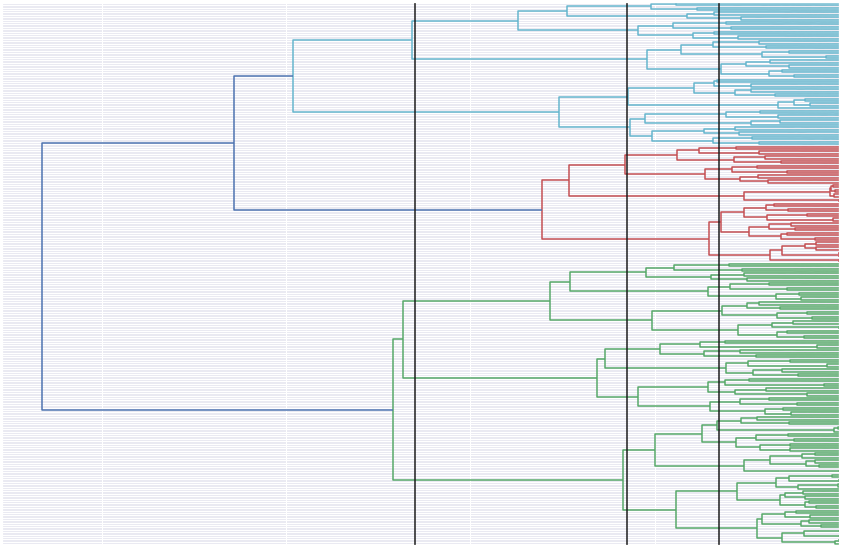
\includegraphics[width=\textwidth]{img/dendrogram_contact_lens}
\caption{Dendrogram computed on the contact lens dataset. The cutoff values for three detail levels are shown in black.}
\label{fig:dendrogram_contact_lens}
\end{figure}

\begin{figure}[!]
\centering
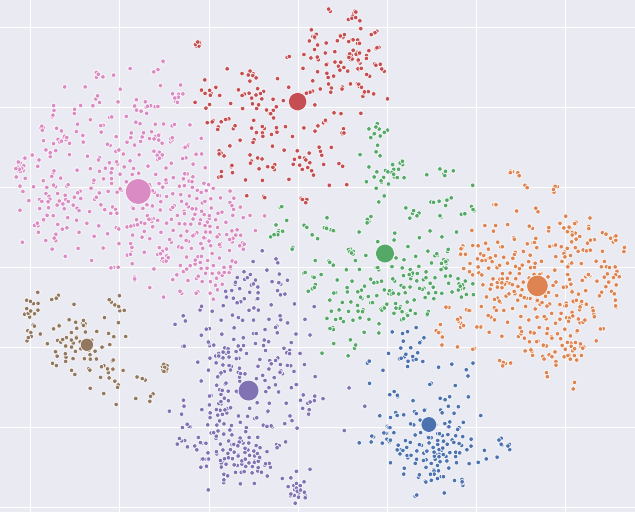
\includegraphics[width=\textwidth]{img/contact_lens_large}
\caption{The most abstract detail level (large clusters) of a clustering on the contact lens dataset. Each cluster has its own color. The circles represent cluster centroids and their radius corresponds to the number of documents within the cluster.}
\label{fig:contact_lens_large}
\end{figure}

To make the similarities between patents within a cluster explicit for the user, we summarize key terms from documents within the cluster to a list of cluster key terms.
As described in \autoref{subsubsec:points} ``Labels'', patent documents are characterized by a list of the 10 most relevant key terms as computed by \gls{tf-idf}.
Across the cluster, we count the occurrences of each term within those 10 document terms.
The 15 most frequently occurring key terms are considered most relevant for the given cluster.
This approach results in more general and common key terms for large clusters, with the specificity growing with each level of detail.

As described in \autoref{subsubsec:clusters}, we augment cluster key terms with similar words to put them into context and avoid ambiguity.
For that, we extract the 10 most similar words from the word2vec model used previously as candidates.
Most similar in this case means that the cosine similarities between word embedding vectors are maximal.
This is the most computationally expensive step in the pipeline since the similarity has to be computed for every single word in the model's vocabulary and for every cluster key term.
If a candidate appears in more than 10\% of documents in a cluster, it is considered an adequate enhancement for the given cluster key term.
Since the word2vec model we use only takes single words into account and does not contain embeddings for multi-word units, bigrams cannot be augmented this way.

The interviews with the patent experts showed that during a patent search, they describe the concept they search for in different levels of abstractness, e. g. umbrella terms and narrower terms (see \autoref{subsec:participant_alpha} and \autoref{subsec:participant_gamma}).
To aid the user's understanding of key terms we attempted to produce generalizations of cluster key terms which are called \textit{hypernyms}.
For example, \textit{chair} is a kind of \textit{furniture}, so \textit{furniture} is a hypernym for \textit{chair}.
These kinds of relationships between words in the English language have been manually captured in the WordNet database \cite{wordnet}.
Our attempt resulted in very similar hypernyms for all clusters that were too general to be useful, for example \textit{speed, base, length, element, metal, gas, velocity, constant, concentration}.
For this reason, we did not pursue this research direction further.

\section{Implementation of the user interface}
\label{sec:user_interface_concept}

In this section, we describe each component of the proposed visualization layout separately.
We examine how the dimensions of data are mapped to visual attributes.
We then describe how the views are coordinated through the way they react to user interactions.

A schematic representation of the visualization layout is shown in \autoref{fig:schematic}.
The layout consists of two columns and each of them is split into two rows as shown in \autoref{fig:columns_rows_layout}.
The first column takes 75\% of the screen's width and contains the scatter plot (80\% of the total height) and the histogram (20\% of the total height).
The second column fills the remaining 25\% of the total width and contains the sunburst with breadcrumbs in the top two-thirds and the detail view in the bottom third.
In the early versions of the prototype, the width and height of the layout's elements were fixed.
Later, we switched to relative sizes to become independent of the exact screen dimensions.
Nevertheless, the prototype is best viewed within a range of resolutions from 1600x900 to 1920x1080 pixels on a screen diagonal from 14 to 24 inches.
The main restriction to arbitrary scalability are the font sizes used in the user interface.
With resolutions smaller than mentioned above the overlap between text elements is likely to harm readability.
With larger resolutions text and point elements will be too small, but it can be alleviated by magnifying the whole web page.

\begin{figure}[!]
\centering
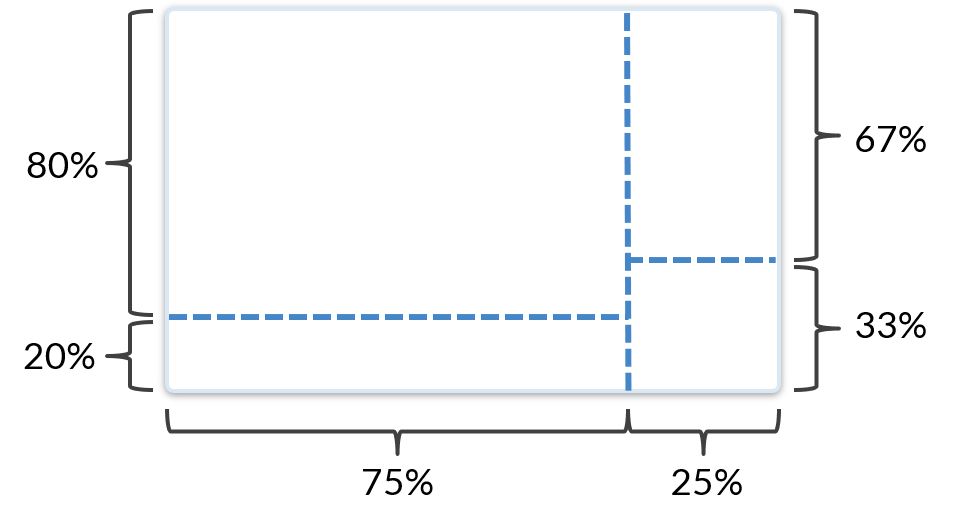
\includegraphics[width=0.6\textwidth]{img/columns_rows_layout}
\caption{Proportions of rows and columns in the dynamic layout.}
\label{fig:columns_rows_layout}
\end{figure}

\subsection{Scatter plot}
\label{subsec:scatter_plot}

The scatter plot is the main area of the visualization and is complemented by all other elements: histogram, sunburst + breadcrumbs and detail view.
It represents each patent as a point with coordinates that correspond to its position after dimension reduction with \gls{tsne}.
Additionally, points are grouped into clusters, each of which is indicated by its key terms.
In this subsection we discuss the depiction of single patents first. 
We then proceed to describe cluster representations.

\subsubsection{Points}
\label{subsubsec:points}
Each data point possesses multiple visual dimensions: position, size, color. 
In the following paragraphs we describe how they are mapped to dimensions of the data.
As mentioned before, the position corresponds to the coordinates in the semantic document space reduced to two dimensions.
Size and color are also utilized (see ``Size'', ``Color and glyphs'').\todo{cite suitability of visual dimensions}
They are complemented by connections between patents (see ``Connections'').
Lastly, each point is labeled with the top key terms of the corresponding patent.

\paragraph{Size}~\\
The size of a point depends on the number of forward and backward citations the patent has, all summed up.
The radius of the circle varies between 3 and 9 pixels when no zoom is applied.
The exact scale used in this mapping is dynamic and dependent on the dataset. 
The minimum size always corresponds to the lowest number of citations found per patent in the dataset and the maximum size to the highest number.
The interpolation between the two values is linear.
It is not uncommon for a patent to list hundreds of citations.
With this relative scale, we make sure that the size difference is always obvious to the user, regardless of whether the maximum number of citations per patent in the current dataset is 20 or 900.

\paragraph{Color and glyphs}~\\
Color of the points is a dynamic variable which is defined by the current state of the sunburst's hierarchy.
Specifically, whenever the user navigates to a different sunburst node, colors are newly assigned for its child nodes.
Patents that are outside of the scope of the current node are then completely hidden.
The remaining points in the scatter plot obtain their color depending on their value of the corresponding metadata attribute.

Earlier iterations of the prototype did not include a solution for displaying patents with multiple values of the given attribute.
Instead, they were assigned to the color of the least frequent attribute value.
The intuition behind this solution was to provide visibility to a group that otherwise would be less noticeable, especially if those least frequent values only occur in combination with others.

Eventually, we implemented \textit{glyphs} as a solution for the issue of multiple attribute values.
``A glyph is a graphical object designed to convey multiple data values'' \cite{ware2004information}.
Usually, glyphs possess multiple visual attributes such as color, position or length, which are mapped to different dimensions of the data.
In our case, however, they are restricted to depict only one dimension of the data, which can acquire one or more values.

Our proposed glyphs are depicted in the form of pie charts with a number of slices corresponding to the number of attribute values.
The slices are equally sized since all values of a given attribute are equally meaningful.
Since we wanted to keep the patent representations uniformly shaped, a circular multi-colored pie chart was an obvious enhancement of a single-colored circle.
The idea was also partially inspired by \cite{Dou2011}, where pie glyphs show the distribution of topics within a document. 

Naturally, the question about legibility of pie charts arose. 
If they were to contain too many slices, they would be impossible to decipher.
To check this, we computed the distribution of how many different values patents included for assignees and \gls{ipc} classes (see \autoref{fig:list_distribution}).
The values presented were computed on the contact lens dataset which is described in \autoref{subsec:data_source}, but they do not vary greatly between datasets.

On average, there are 1.56 assignees per patent, with an overwhelming majority of patents having only one assignee.
\gls{ipc} classes on the first glance look unsuitable for a pie chart with an average of 4.92 \gls{ipc} classes per document and a non-negligible amount of patents with more than 20 \gls{ipc} classes.
However, these numbers refer to unique \gls{ipc} classes throughout the whole \gls{ipc} hierarchy.
In reality, only one \gls{ipc} level is visible at one time, so we examined distributions after the first subdivision and before the last one to see how many classes truly have to be shown simultaneously.
On the subdivision level with single \gls{ipc} letters (e.g. A or B) there is an average of 1.87 values per patent, and on the group level (e.g. A21B1 vs. A21C3) it is 3.34, respectively.
This shows that in total, there is relatively little branching throughout the \gls{ipc} hierarchy with most of it happening on the last level. 
This means that the number of slices in a pie chart on each specific \gls{ipc} level is not too high for intelligibility.

\begin{figure}
    \centering
    \subfigure[Assignee]
    {
        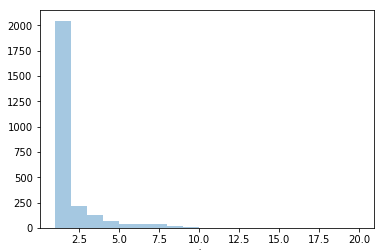
\includegraphics[width=0.45\textwidth]{img/assignees_distribution}
        \label{fig:assignees_distribution}
    }
    \subfigure[\gls{ipc} class]
    {
        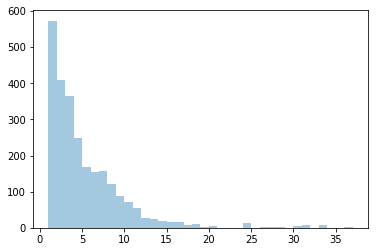
\includegraphics[width=0.45\textwidth]{img/ipc_classes_distribution}
        \label{fig:ipc_classes_distribution}
    }\\
    \subfigure[First letter of \gls{ipc} class (section)]
    {
        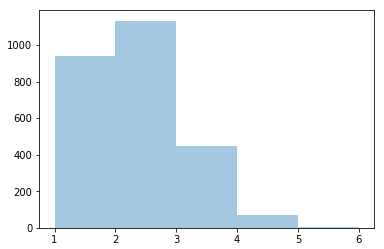
\includegraphics[width=0.45\textwidth]{img/first_letters_distribution}
        \label{fig:first_letters_distribution}
    }
    \subfigure[\gls{ipc} class on group level (4-6 characters)]
    {
        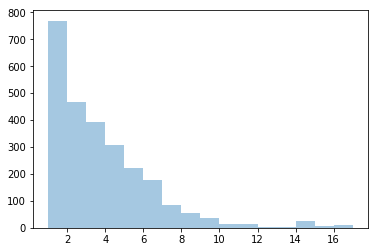
\includegraphics[width=0.45\textwidth]{img/before_slash_distribution}
        \label{fig:before_slash_distribution}
    }
    \caption{The distribution of the number of values per patent for assignee and \gls{ipc} class.}
    \label{fig:list_distribution}
\end{figure}

Using glyphs results in continuous areas with the same glyph appearance (see \autoref{fig:glyphs_areas}), which allows the users to make generalized assumptions about the content of those areas.
We evaluate how well glyphs fulfill their purpose in \autoref{subsubsec:hypothesis2}.
For simplicity, we refer to glyphs as points whenever the multiple attribute values are not essential to the current discussion.

\begin{figure}[!]
\centering
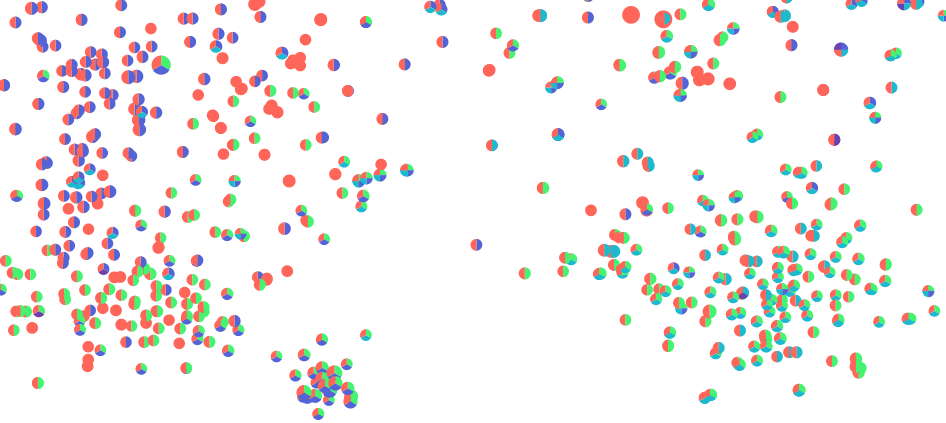
\includegraphics[width=\textwidth]{img/glyphs_areas}
\caption{Areas consisting of same kinds of glyphs on the contact lens dataset.}
\label{fig:glyphs_areas}
\end{figure}

\paragraph{Connections}~\\
Three kinds of possible connections between any pair of patents exist (see \autoref{fig:lines}).

\begin{figure}[!]
\centering
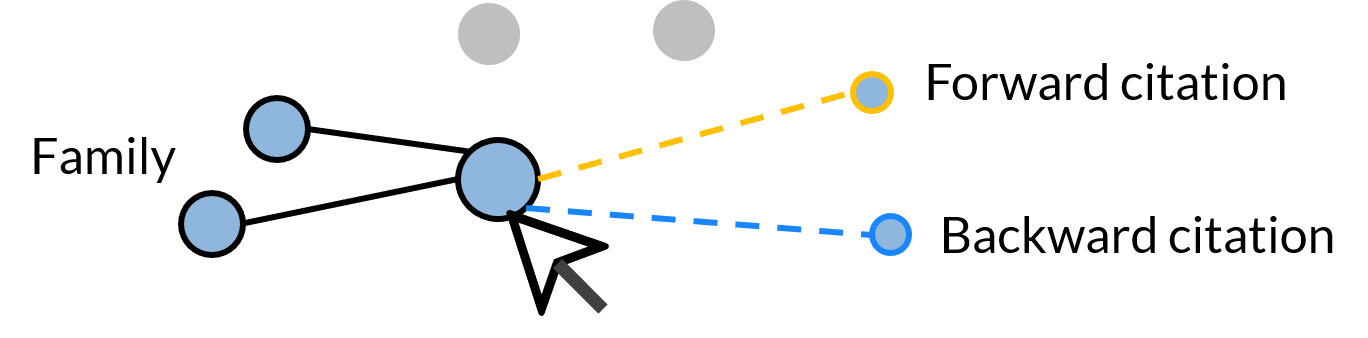
\includegraphics[width=0.7\textwidth]{img/lines}
\caption{Various kinds of connections between patents.}
\label{fig:lines}
\end{figure}

As described in \autoref{subsubsec:patent_family_and_priority_document}, patent families describe the same invention.
Being the same family is the strongest indication of a semantic similarity, which is why families mostly are represented by close-knit groups of points in our semantic approach.
We show connections to other family members with black solid lines.

Citations are another kind of possible connection between patents.
As opposed to family connections, they do have a direction.
Conventionally directed connections are shown with arrows, which is inapplicable in our case.
A single patent might have tens to hundreds of citations, which would result in a very cluttered representation if arrows were used.
Moreover, it is useful to be able to see at a glance the areas where the majority of citations come from and go to.
As described \autoref{subsubsec:forward_backward_citations}, if a new patent application cites an existing patent, it means the inventors are aware of the prior invention and see the novelty in their invention with regards to the prior invention.
This is called \textit{forward citation}, which we show with a yellow dashed line.
The opposite situation, i. e. from the point of view of an older patent, is a \textit{backward citation} shown with a blue dashed line.

We chose complementary colors (blue and yellow) because they signify exactly opposite things - opposite directions of citation.
Yellow is more of an ``active'' color, which signifies that currently selected patent explicitly mentions the citation.
Blue has a more ``passive'' role, which in our case corresponds to the fact that backward citations are not directly contained in the data, but are instead computed by reversing the connections.
Notably, yellow and blue both can be easily seen on black background.
It so happens that some patents are listed as both family members and citations, so dashed lines are designed to overlay the black lines and still be clearly distinguishable.
Additionally, a dashed line is usually perceived as less important than a solid line, which correctly represents the domain knowledge in this case.

Connections appear while the user is hovering over a patent with a mouse.
The user can also choose to select a patent by clicking on it.
In this case, the connections persist until the user switches their selection to another patent or resets the selection completely by clicking on the background area of the scatter plot.
The selection mode allows the user to highlight a patent of choice and examine its citations and family by hovering the mouse over them.
This interaction implements the principles of \textit{focus plus context} (explained in \autoref{subsubsec:focus_context}) and \textit{details on demand} (explained in \autoref{subsubsec:visual_information_seeking_mantra}).
The chosen patent is in focus and its citations and family provide a more detailed representation and also show some context, i. e. what prior art the patent refers to.

\paragraph{Labels}~\\
Each patent has a corresponding label that shows up to three top key terms as extracted by the TF-IDF algorithm (see  \autoref{subsec:term_extraction} for details).
Information density is an essential characteristic of any user interface that directly impacts usability.
To avoid cluttering the visualization space, we use use a heuristic to determine exactly what labels are shown and how many top key terms they include.

Our experiments showed that about 250 labels (consisting of one key term) for points can be shown simultaneously and remain mostly readable. 
So we decided to limit the labels to a maximum of 250.
This means that some points are shown unlabeled until the user restricted the area they are interested in to under 250 patents.
After each operation, such as filtering, panning or zooming, we count the points that are currently situated within the viewport.
We then divide that amount by 250.
If the resulting quotient $q$ is over 1, we round it up to the next integer to get $n$.
In this case, every $n$th point is labeled with its top key term. 
For example, if 980 patents are currently visible, every 4th of them gets labeled, and three-fourths of patents are shown with just a point without a label.
If $q$ is between 0.7 and 1, every patent in view is labeled with its top key term.
Usually, this happens during the examination of small clusters (see \autoref{subsec:hierarchical_clustering} for explanation of three cluster sizes), when the user's attention shifts to a single document.
For values of $q$ between 0.3 and 0.7, there is sufficient space for top two key terms and for values under 0.3 for three top key terms for every patent.

The above-mentioned value intervals are chosen to maintain a visual balance between points and their labels and to minimize overlapping text.
If the user wishes to examine further key terms beside the top three ones, they have the possibility to inspect them in the detail view (described in \autoref{subsec:detail_view}) along with complete information about the patent.
We provide the possibility for the user to comprehend the distribution of points and their colors without distraction before starting with the detailed analysis. 
To support this, we make all point labels invisible when the zoom level is less than 1.15.

The varying number and length of patent key terms result in a dynamic level of detail.
It is one of our multiple embodiments of the \textit{semantic zooming} mechanism (explained in \autoref{subsubsec:semantic_zooming}).
The evaluation (see \autoref{subsubsec:hypothesis5}) showed that our heuristic resulted in a readable representation for multiple levels of detail.

\paragraph{Zooming}~\\
Zooming causes a multiplicator to be applied to the point size.
The multiplicator value varies from 1x to 1.7x and is interpolated linearly depending on the exact zoom level.
The maximal possible zoom level is 10, but after it reaches 3, points and text in the scatter plot stop increasing in size, so further magnification only increases the distance between the points.
Thus, we intentionally increase the amount of white space to allow the user to focus their attention on specific patents.
Also, at this detail level, the documents are accompanied by a list of key terms which need to be readable.
Improved readability is also a reason for the additional white space.

The lines representing families and citations also change subtly with the zoom level.
Their width changes from 2 to 3 pixels to stay in proportion with the point size.

To allow users to quickly go back to the overview of the dataset, we added a ``Reset zoom'' button in the latest iteration of the concept.
This way, the users are able to go set the zoom level back to 1 with one click instead of turning the mouse wheel two to seven times depending on the size of the dataset.
We would like to mention that navigating to the maximum zoom level is rarely, if ever, continuous.
The user pauses to analyze the currently presented information to steer their further examination.
Therefore zooming into the dataset is not as cumbersome as zooming out without using the reset button would be.

\subsubsection{Clusters}
\label{subsubsec:clusters}
As described in \autoref{subsec:hierarchical_clustering}, we cluster patents hierarchically based on their distance in the 2D space, i. e. their proximity in the scatter plot.
From the computed agglomerative clustering we pick three specific cluster configurations, which provides us with three levels of detail.
We refer to them as \textit{large, medium} and \textit{small} cluster sizes.

Clusters are represented in the visualization by their key terms.
Since we are essentially generating a themescape, we considered a solution from the domain of map drawing.
On a map, labels for areas such as forests, deserts or lakes are often not straight but bent to match the shape of the area.
We tried to replicate this behavior by approximating the points in the cluster by a polynomial curve.
The cluster text was supposed to stretch and follow the curve to make the shape of the cluster visible.
The result of our attempts is presented in \autoref{fig:curves}.

\begin{sidewaysfigure}[!]
\centering
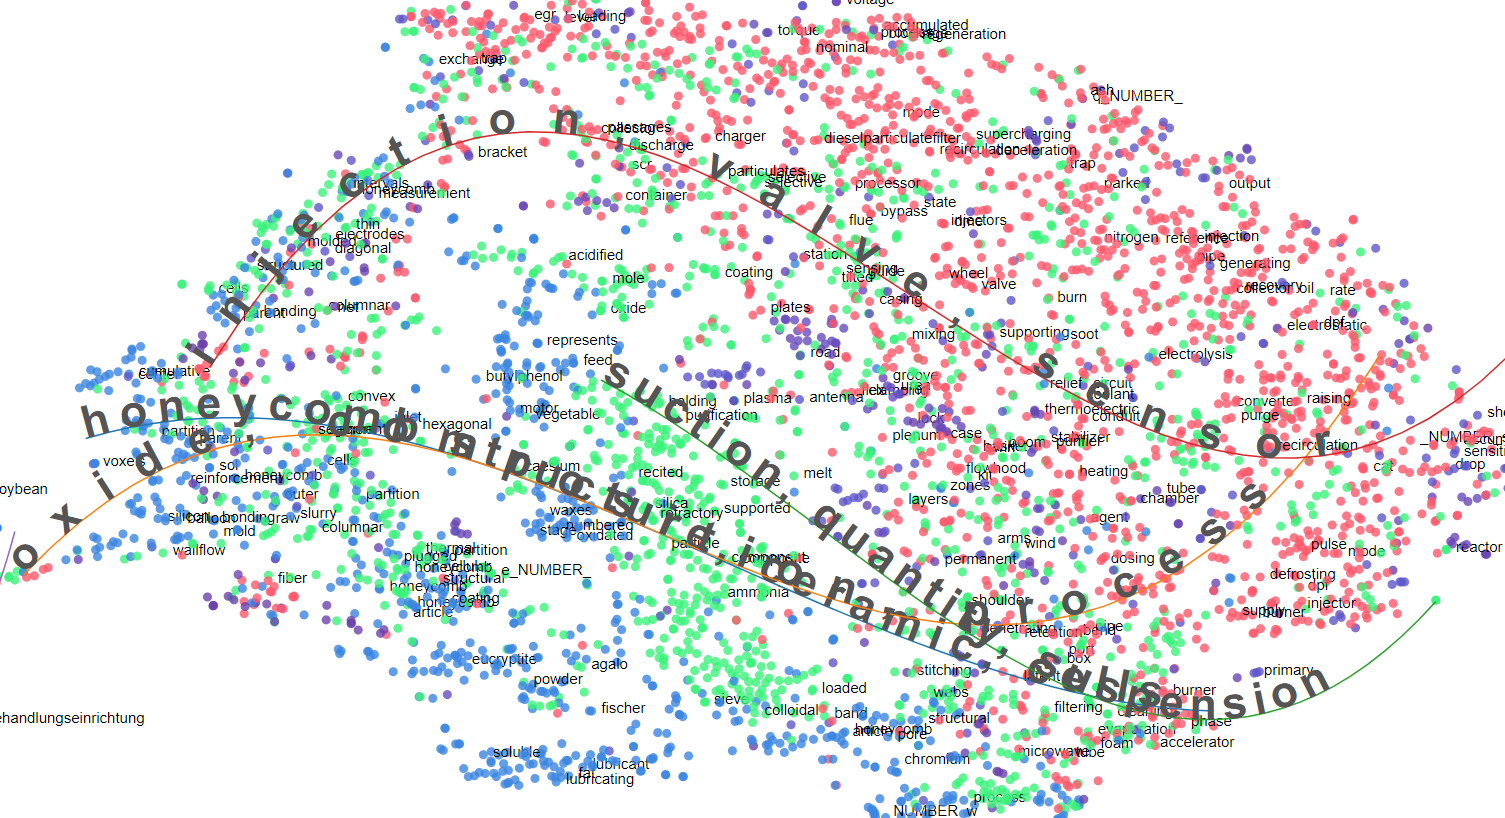
\includegraphics[width=\textwidth]{img/curves}
\caption{Cluster shapes approximated by curves on the diesel engine dataset. The text for cluster labels is placed on the curves.}
\label{fig:curves}
\end{sidewaysfigure}

At that stage, we were computing the whole clustering based on distances in the high-dimensional document space.
With this approach, dimension reduction to 2D resulted in elongated cluster shapes which, as we initially hoped, would be easy to approximate.
At the same time, elongated clusters were not separated clearly and often overlapped, which significantly reduced the quality of the approximating curves and the readability of text placed on them.
It was also difficult to adjust how the text should stretch depending on the length of the key terms and the length of the curve.
For these reasons, we decided not to pursue this direction of research further.
Notably, \cite{Skupin2013} uses the professional \gls{gis} software ArcGIS extended by the Maplex labelling engine to place labels on their themescapes with great success (see \autoref{fig:som} for an example themescape).
This speaks strongly for the potential of applying map drawing methods for non-geographical data.

In the current embodiment of our approach, each cluster is represented by its top three key terms situated exactly in the middle of the cluster.
To place them in a compact way, we show the most relevant term in the middle and complement it by the second and third terms above and below it.
The font size of the top term is bigger by three pixels to emphasize its importance according to principles of visual hierarchy.
Moreover, both visibility and font size differ between large, medium and small cluster labels depending on the current zoom level (see \autoref{table:font_sizes}).

\begin{table}[h!]
\centering
\begin{tabular}{||c c c||} 
 \hline
 Cluster level & Font size, pixels & Visible at zoom level \\ [0.5ex] 
 \hline\hline
 large & 23 to 28 & <1.6 \\ 
 medium & 18 to 22 & 1.5 to 2.1 \\
 small & 14 to 18 & 2.0 to 3 \\ [1ex] 
 \hline
\end{tabular}
\caption{Font sizes for different cluster sizes}
\label{table:font_sizes}
\end{table}

As the user zooms into the scatter plot, bigger clusters are replaced by smaller ones. 
This continues until the zoom level of 3, when the cluster labels disappear completely allowing the user to examine specific patents efficiently.
Notably, the visibility intervals overlap slightly.
This means that briefly, both large and medium or both medium and small cluster labels are seen.
The idea here is to make the transition between different levels of detail smoother.
The font size of cluster labels increases slightly while zooming in.
As mentioned before, points themselves and connections between points also increase in size.
This behavior is implemented in a consistent way throughout the scatter plot to support the feeling of ``moving into'' the dataset.

To optically balance out the increasing line thickness as the clusters labels become larger, we vary the font color slightly.
Labels for single patents are black, so we made little cluster labels a few shades lighter, which yields a dark gray.  
By analogy, medium and large clusters were also assigned gray color slightly lighter than at the corresponding previous level.
A comparison of black and our lighter alternative for large cluster labels can be seen on figures \autoref{fig:cluster_terms_black} and \autoref{fig:cluster_terms_gray}.
Additionally, the distinction between cluster terms and patent terms is accentuated by using unequal colors.
To strengthen the effect and increase readability on a colorful background, we draw a thin white contour around the cluster labels (compare figures \autoref{fig:cluster_terms_nowhite} and \autoref{fig:cluster_terms_gray}).

\begin{figure}
    \centering
    \subfigure[Black text with white contour]
    {
        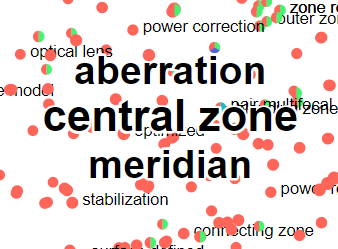
\includegraphics[width=0.4\textwidth]{img/cluster_terms_black}
        \label{fig:cluster_terms_black}
    }
    \subfigure[Gray text without contour]
    {
        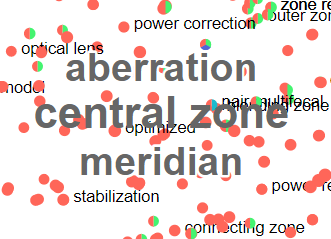
\includegraphics[width=0.4\textwidth]{img/cluster_terms_nowhite}
        \label{fig:cluster_terms_nowhite}
    }
    \subfigure[Gray text with white contour]
    {
        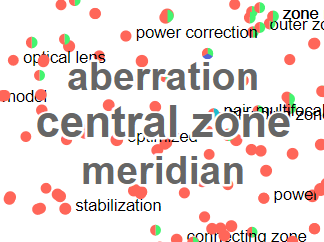
\includegraphics[width=0.4\textwidth]{img/cluster_terms_gray}
        \label{fig:cluster_terms_gray}
    }
    \caption{Font color and contour increase readability of cluster labels.}
    \label{fig:cluster_labels}
\end{figure}

Some of the cluster key terms are assigned a list of \textit{augmenting words} which provide context for occasionally unclear or ambiguous terms (see \autoref{subsec:hierarchical_clustering} for details on augmentation).
This information is not of a high-priority, thus we only display it on demand.
A tooltip with a list of augmenting words appears when and only when the user hovers over the corresponding term with the mouse.
No tooltip is shown when the given term possesses no augmenting words.
Naturally, there has to be a clear indication of what term out of three possible presented is enhanced with a tooltip.
There was no easy technical possibility to show the tooltip on the side of the corresponding term, so we placed it underneath the cluster label.
We make the current state of the interface explicit by highlighting in wine red color the term which the tooltip currently corresponds to as shown in \autoref{fig:tooltips}.

\begin{figure}[!]
\centering
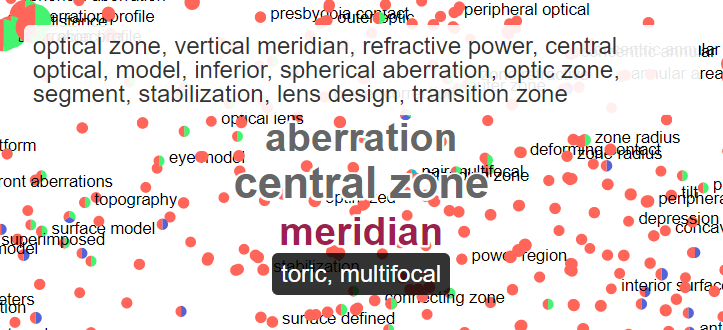
\includegraphics[width=0.8\textwidth]{img/tooltips}
\caption{Tooltip with augmenting words below and tooltip with all cluster terms above}
\label{fig:tooltips}
\end{figure}

Since we actually computed the top 15 key terms per cluster but had only been showing 3 of them so far, we decided to display the remaining 12, too.  
For that purpose, in the latest iteration of the prototype we added another tooltip, this time above the three terms, with distinctly different appearance to avoid any confusion.
The interaction follows the same pattern as with the first tooltip, i. e. it is displayed on mouse hover.

\subsection{Histogram}
\label{subsec:histogram}

The histogram view shows the number of submitted patent applications per year in the form of a bar chart (see \autoref{fig:histogram}).
It is, in fact, a histogram in which the bin size equals one year.
It allows the user to involve the temporal dimension into their perception of the data.
With a brushing interaction, the user can filter out the data outside the selected interval.
The selected window can be moved or expanded with the help of the handles on either side.
With a click on the background of the histogram the selection can be reset.
On the X-axis, only every second year is labeled to avoid overcrowding.
To compensate for that, the years of a current selection are shown in the upper-left corner.
It helps eliminate the need for mental computations as the user chooses a time interval of interest.

\begin{figure}[!]
\centering
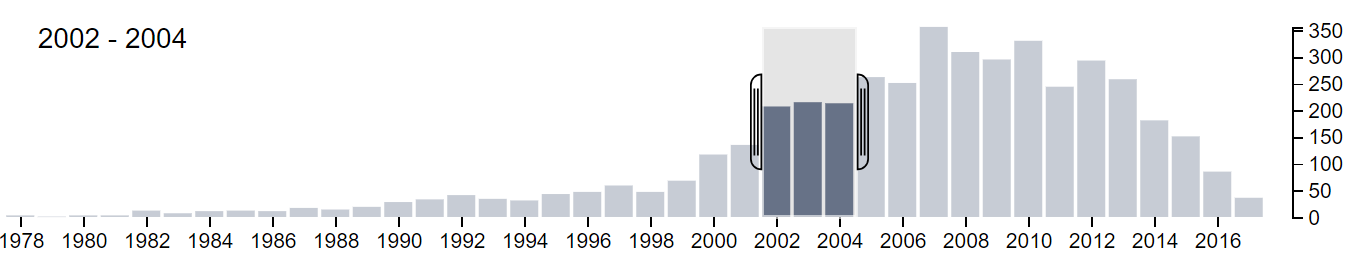
\includegraphics[width=\textwidth]{img/histogram}
\caption{Histogram view as seen on diesel engine dataset. The time interval from 2002 to 2004 is selected.}
\label{fig:histogram}
\end{figure}

The values in the histogram are computed based on the current top node in the sunburst.
Initially, the top node corresponds to the whole dataset, and then switches to its specific portions as the user focuses their attention on specific metadata attribute values.
The scale of the Y-axis of the histogram is adjusted dynamically as its maximum value changes.
Additionally, the histogram is directly involved in other forms of interactions between views that are described in \autoref{sec:interactions_between_views}.

\subsection{Sunburst and breadcrumbs}
\label{subsec:sunburst_and_breadcrumbs}

\subsubsection{Sunburst}
\label{subsubsec:sunburst}
Our implementation of sunburst is based on interactive demos from \cite{Asturiano} and \cite{Trott}.
The angle taken by nodes is linearly dependent on the number of patents that have the corresponding attribute value.
The nodes are sorted by their value in the descending order.
When there is enough space available, node names are displayed in the center of a node.
The text follows the node's arc and is surrounded by a white contour for a better readability.
The title of the node and an absolute number of patents belonging to it are also shown as a tooltip when the user hovers over the node.

The color of nodes on the first sunburst level is based on a cyclical rainbow color palette.
Basically, the angles within the interval $[0\textdegree, 360\textdegree]$ are mapped to a corresponding position from $[0, 1]$ on the color scale.
A node's angle for the purpose of this calculation starts at 0\textdegree and ends in the middle of the node's arch where its title is.
Because the color scale is cyclical, nodes nearing 360\textdegree have similar colors to those near 0\textdegree.
Child nodes expanding from the first sunburst level are assigned a spectrum of shades from darker than parent to lighter than parent.
This emphasizes that they belong to the parent.

When patents possess multiple values of the same attribute, for example, assignee or \gls{ipc} class, occurrences of each single value are bound to exceed the number of patents when summed up.
To represent that overlap correctly, we normalize the values so that they add up to a total of 100\%.
For example, assume there are two assignees A and B in a dataset, 80\% of patents have A as their assignee and 40\% have B.
This means that 20\% of patents have been submitted by A and B together.
To correctly represent the relative distribution, we would draw node A as $\frac{80}{80+40=120} = 67\%$ of the sunburst and node B as $\frac{40}{120} = 33\%$.

It is possible to navigate to deeper hierarchy levels by clicking on the chosen node.
To go back one level, the user needs to click on the circle in the middle of the sunburst which represents the current top node.
The transitions between two states are animated to emphasize the change in the system state: sunburst nodes fold and unfold like a fan.
Change in the state of the sunburst also directly affects the scatter plot: first, only points belonging to the currently chosen node stay visible, second, their colors change to match the new sunburst nodes.
In addition to clicking, the user can also hover over a sunburst node to see a preview of their choice.
In this case, not related patents are hidden in the same way as with clicking, but point colors stay as they are because the sunburst nodes have not yet changed their colors.
Only the nodes on the path to the currently highlighted node retain their color.
Remaining nodes are shown with a lighter color to keep all focus on the highlight.
The highlight is reset after the user moves the mouse outside of the sunburst's circle.

\subsubsection{Breadcrumbs}
\label{subsubsec:breadcrumbs}
\textit{Visibility of system status} and \textit{recognition over recall} are two of usability expert Jakob Nielsen's ten heuristics for user interface design \cite{Nielsen1994}. 
To take them into account, the first change from the initial concept was adding \textit{breadcrumbs} to the sunburst view.

Breadcrumbs are a metaphor most familiar to users from website navigation (see \autoref{fig:breadcrumb_examples} for examples).
The name originates from the German fairy tale about Hansel and Gretel, who left a trail of bread crumbs in the woods to be able to find their way back \cite{levene2011introduction}.
Breadcrumbs are applicable with hierarchically arranged navigation, i. e. when there is only one possible path to every node in the navigation tree.
According to \cite{Gube2019}, they are usually used as an optional aid to navigation and should be less prominent than the primary navigation element (which is the sunburst in our case).

\begin{figure}[!]
\centering
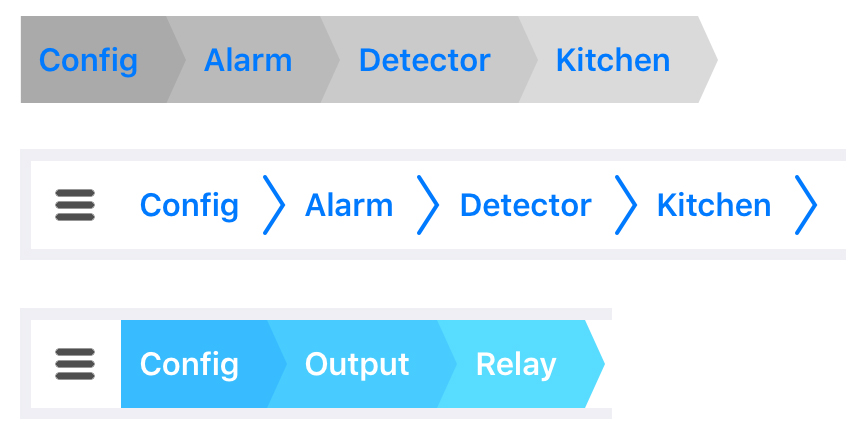
\includegraphics[width=0.5\textwidth]{img/breadcrumb_examples}
\caption{Different kinds of breadcrumb design. Image source:\cite{breadcrumb}}
\label{fig:breadcrumb_examples}
\end{figure}

With the first implementation of the sunburst, it soon became clear that some hierarchy nodes were too narrow to include their title within.
Moreover, the titles that could be shown were placed at different angles, which prevented a sequence of highlighted nodes from being read easily.
Breadcrumbs build a straight line, which increases readability.
Additionally, when a user switches to a deeper level of the sunburst hierarchy, the parent nodes are no longer visible. 
In accordance with the \textit{recognition over recall} principle, it should not be expected of any user to remember what parent nodes came before.
We included breadcrumbs as a visual aid that clearly and consistently represents the status of the system and reassures the users of the result of their actions, especially when they interact with small sunburst nodes.
The result can be seen in \autoref{fig:breadcrumbs_without_text}.
A percentage on the right side of the breadcrumb trail represents the fraction of patents from the currently highlighted hierarchy node with regard to the current root node.
It is especially useful when there is a significant overlap between node values because it shows the true value of the node independent of its normalized angle.

\begin{figure}[!]
\centering
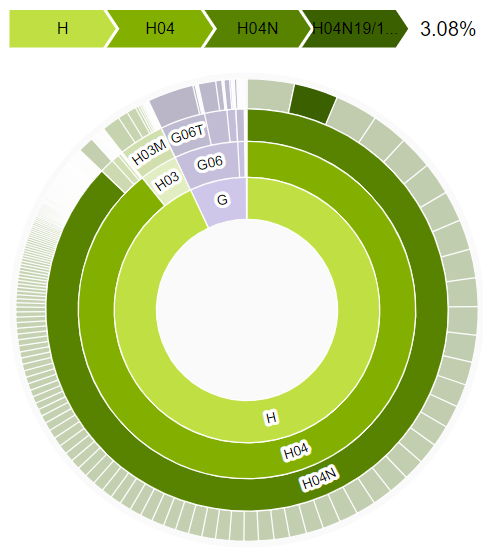
\includegraphics[width=0.7\textwidth]{img/breadcrumbs_without_text}
\caption{First version of breadcrumbs complementing the sunburst view.}
\label{fig:breadcrumbs_without_text}
\end{figure}

Short codes for \gls{ipc} classes fit well into the width of the line allocated to them.
To keep the breadcrumbs view concise for assignees as well, we chose only to show the first nine characters of a node's title followed by an ellipsis mark.
As assignee names can be over 30 characters long, the need to see full node titles remains.
The idea proposed by patent experts during a feedback meeting helped address this issue.
The experts wished to see full descriptions for \gls{ipc} codes, for example, ``optical elements, systems, or apparatus'' for class G02B (see \cite{ipc} for full schema).
This led us to complement the graphical brief breadcrumbs with a full-text part as seen in \autoref{fig:breadcrumbs_text}.
Full assignee names could then be shown completely along the \gls{ipc} descriptions.

\begin{figure}[!]
\centering
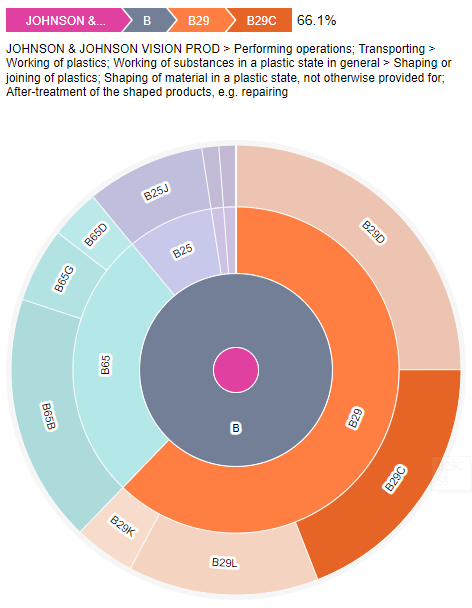
\includegraphics[width=0.8\textwidth]{img/breadcrumbs_text}
\caption{Full-text titles of sunburst nodes added to breadcrumbs.}
\label{fig:breadcrumbs_text}
\end{figure}

\subsection{Detail view}
\label{subsec:detail_view}

The detail view follows the principle of \textit{details on demand} (see \autoref{subsubsec:visual_information_seeking_mantra} for details). 
It allows the user to examine all of the available metadata per patent.
The information is organized in a tabular manner for compactness (see \autoref{fig:detail_view}).
Included are (left to right, top to bottom) publication number, title, application date, a list of assignees, forward and backward citations, a list of \gls{ipc} classes,  a list of the top 15 relevant key terms and the abstract.

\begin{figure}[!]
\centering
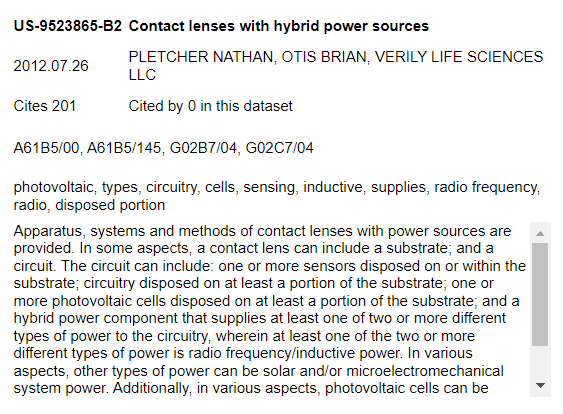
\includegraphics[width=0.8\textwidth]{img/detail_view}
\caption{Detail view on an example patent from the contact lens dataset.}
\label{fig:detail_view}
\end{figure}

If the user would like to study the patent text thoroughly, they can double-click anywhere in the detail view.
This causes an additional browser window to appear, which contains the full text of the textual parts of the patent, i. e. abstract and claims (see \autoref{fig:claims}).
When the user double-clicks on another patent, the already opened window persists and a new one is opened.
This permits a detailed examination and comparison of multiple patents.

\begin{figure}[!]
\centering
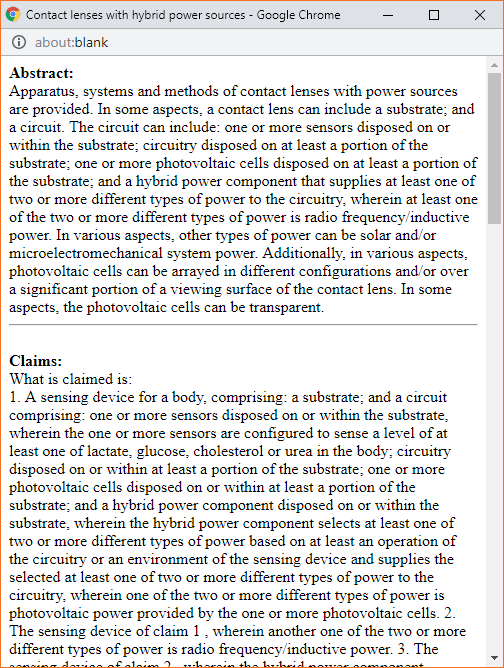
\includegraphics[width=0.8\textwidth]{img/claims}
\caption{Window with full text (abstract and claims) of an example patent from the contact lens dataset.}
\label{fig:claims}
\end{figure}

\subsection{Interactions between views}
\label{sec:interactions_between_views}

For a consistent behavior across all parts of the interface, we enable similar kinds of interactions for the sunburst, the histogram and the scatter plot.
We distinguish between three kinds of interactions:
\begin{itemize}
\item hovering over an object for a preview of the changes - ``Highlighting''
\item clicking on an object to make the change persistent - ``Selecting''
\item clicking on a background of the view to reset the selection.
\end{itemize}
An overview of how those interactions influence coordinated views is shown in \autoref{fig:interactions_between_views}.
In this section we describe the possible user actions that had not yet been covered in the previous sectionss.

\begin{figure}[!]
\centering
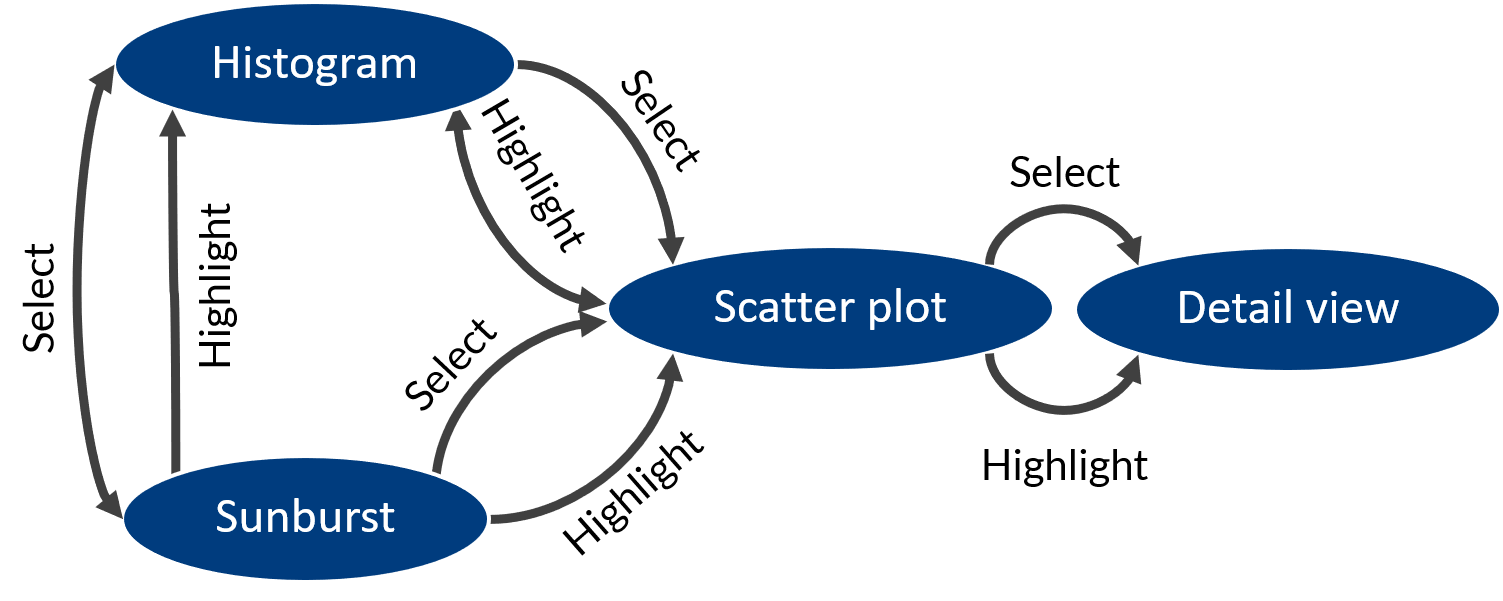
\includegraphics[width=0.8\textwidth]{img/interactions_between_views}
\caption{Diagram of interactions between views. The arrows point from the view where the given interaction happens to the view where it takes effect.}
\label{fig:interactions_between_views}
\end{figure}

On a histogram, the user can select a certain time interval by brushing.
The histogram bars for the years outside the selection become grayed out, so do the patents submitted outside the selected interval.
Then, the sunburst is generated anew based only on the patents within the selection.
The colors of the remaining points then adjust to match the new state of the sunburst.
See \autoref{fig:histogram_brushing_interaction} for a comparison of states before and after brushing.
In this example, one can see that patents submitted from 2007 to 2011 are concentrated in one thematic area.
Moreover, less of them are assigned the \gls{ipc} class G - ``Physics'', while H - ``Electricity'' becomes more widespread.
This might be an indication of a change in the meaning of the \gls{ipc} classes over time: the first version of \gls{ipc} classification was developed in 1968 before the rapid development of information technology.
The selection in the histogram can be reset by clicking on its background.

\begin{figure}[!]
    \centering
    \subfigure[Before brushing]
    {
        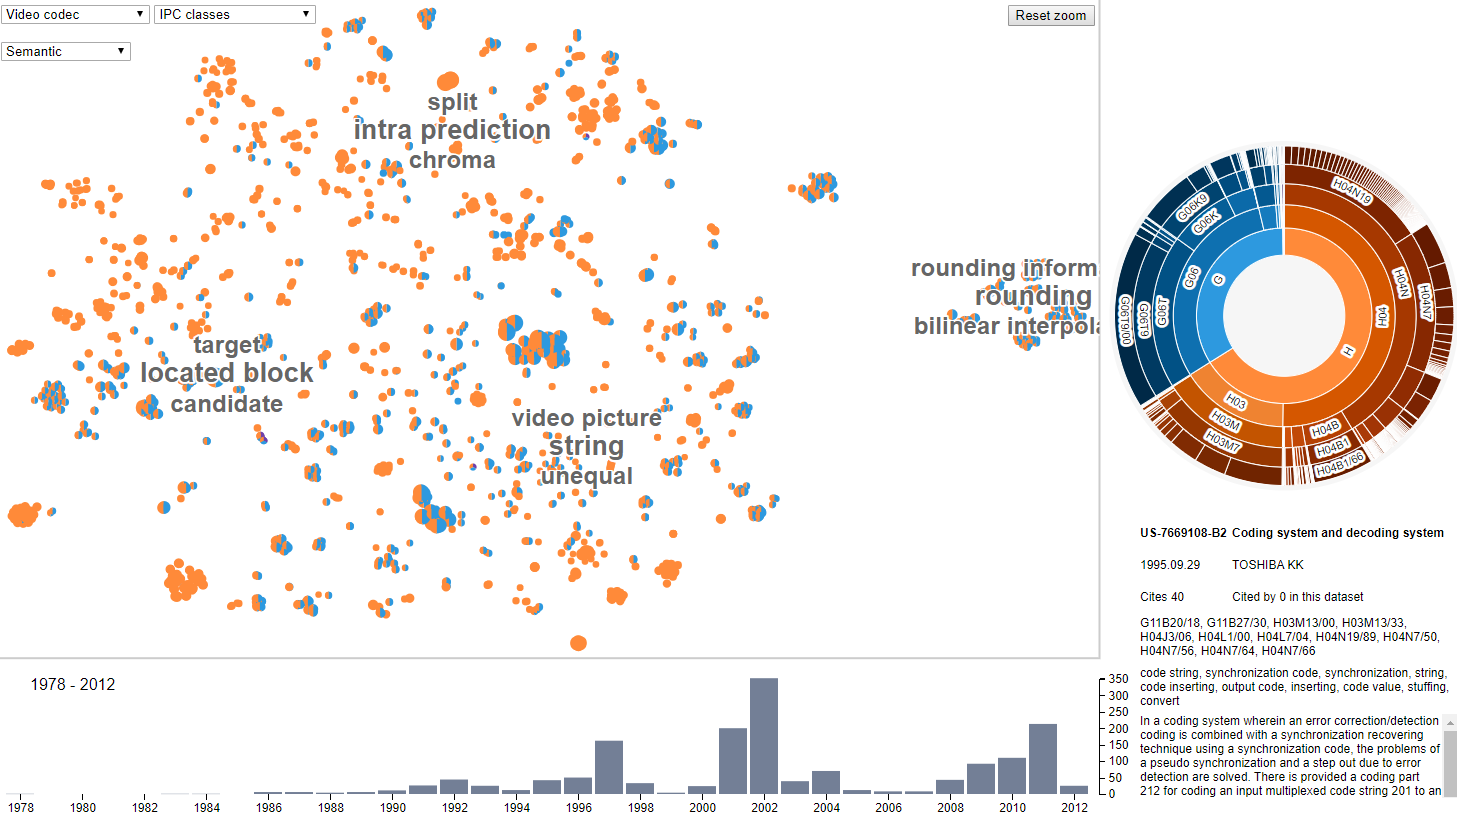
\includegraphics[width=\textwidth]{img/histogram_before_brush}
        \label{fig:histogram_before_brush}
    }\\
    \subfigure[After brushing]
    {
        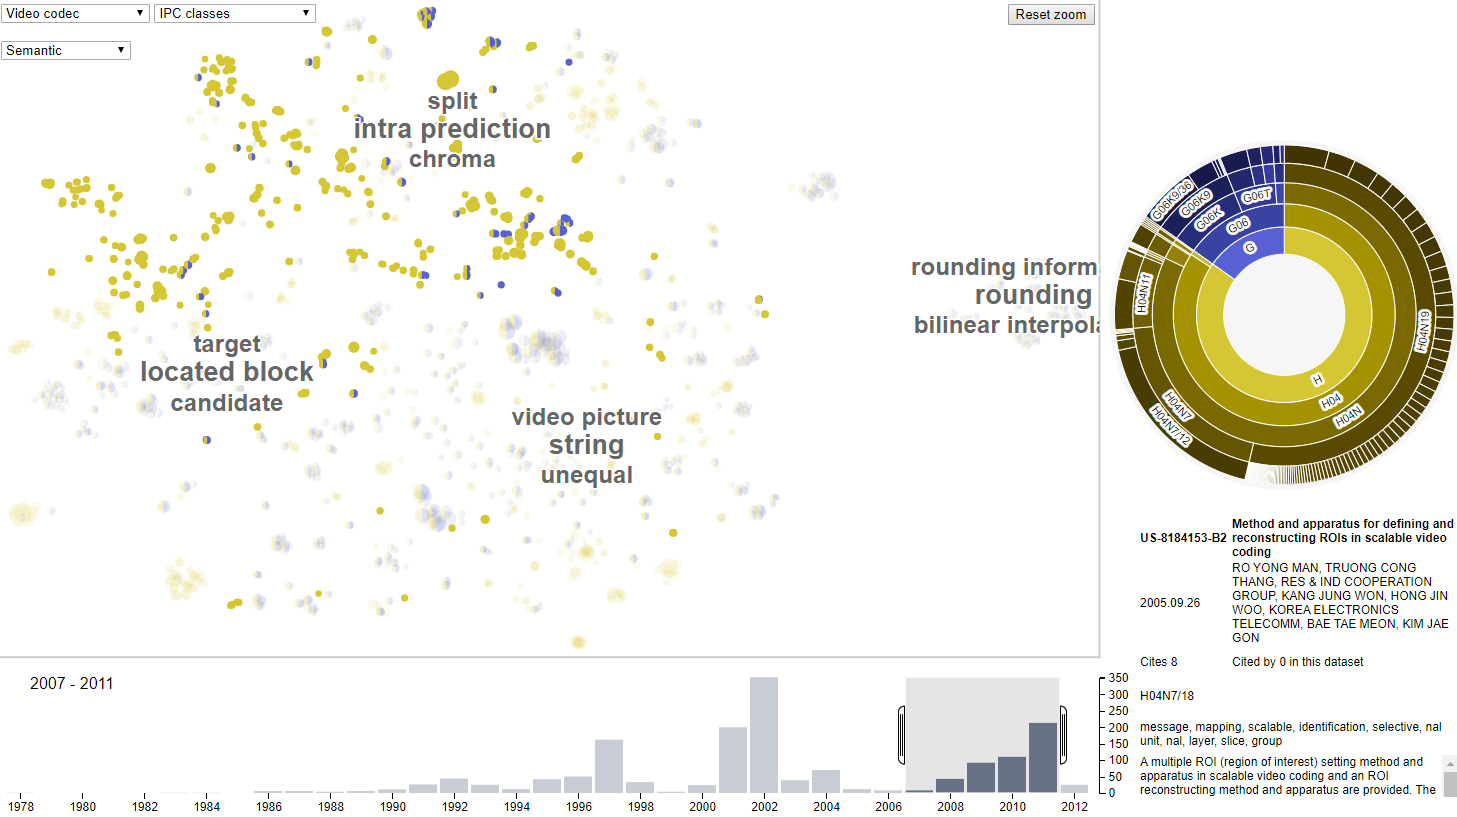
\includegraphics[width=\textwidth]{img/histogram_after_brush}
        \label{fig:histogram_after_brush}
    }
    \caption{The impact of a brushing action on a histogram on the scatter plot and sunburst. Video codec dataset}
    \label{fig:histogram_brushing_interaction}
\end{figure}

When the user hovers over a sunburst node, this node's contribution to the histogram is displayed in the color corresponding to the sunburst node.
In other words, the histogram becomes a stacked bar chart in which the bottom part of the stack corresponds to the highlighted sunburst node and the upper part of the stack includes all other patents.
This interaction allows the user to follow the temporal trends in the development of a single \gls{ipc} class, assignee or country.
For example, Figure \autoref{fig:sunburst_hover} shows that 3D printing technology has started developing rapidly in China since 2015.
If the user then clicks on China, it moves to the center of the sunburst and its children take over the whole circle.
The bars corresponding to China that were blue on hover now constitute the whole histogram and the Y-axis is scaled accordingly (see Figure \autoref{fig:sunburst_click}).
Moreover, the points in the scatter plot now match their colors to the child nodes of China.

\begin{figure}[!]
    \centering
    \subfigure[While hovering]
    {
        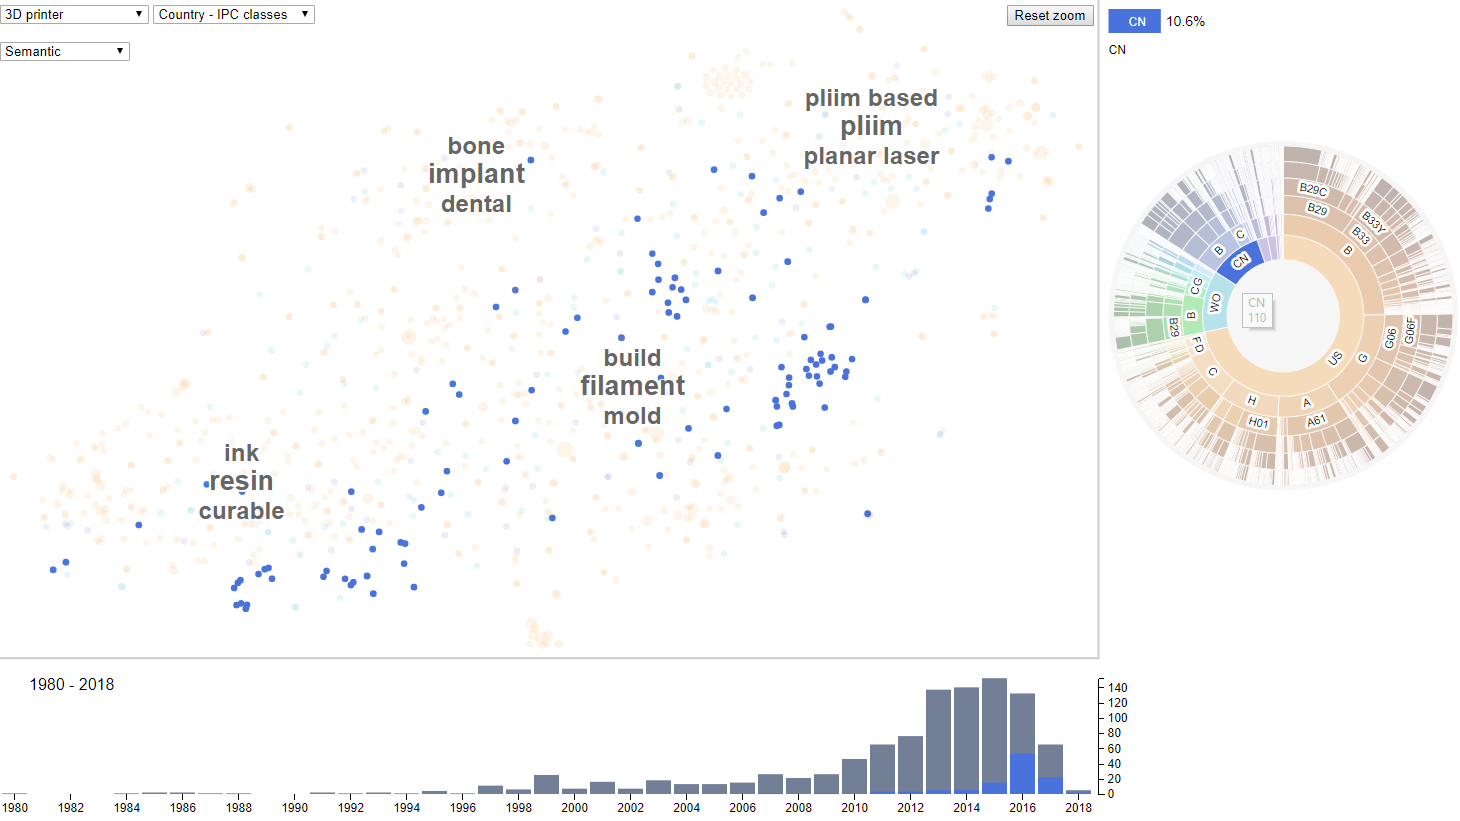
\includegraphics[width=\textwidth]{img/sunburst_hover}
        \label{fig:sunburst_hover}
    }\\
    \subfigure[After clicking]
    {
        \includegraphics[width=\textwidth]{img/sunburst_click}
        \label{fig:sunburst_click}
    }
    \caption{The impact of hovering and clicking on a sunburst node on histogram and scatter plot. 3D printer dataset}
    \label{fig:sunburst_interactions}
\end{figure}

The scatter plot also implements the highlighting and selection with regard to single patents.
As long as the user hovers over a certain point, it is emphasized by a black contour and its citations and family members become visible.
The detail view then shows the metadata of this particular point, but the information persists even when the mouse is taken away until some other patent is highlighted.
Moreover, the year when the patent was submitted is accented in bright yellow on the histogram (see Figure \autoref{fig:sunburst_click}).
It gives the user a quick impression about the age of the patent without the need to read this information in textual form in the detail view.
Clicking on a patent makes its connections permanently visible.
The user is then able to examine related patents by hovering over them.
The detail view is reset to the details of the selected point when no other point is hovered over.
A click on a background of the scatter plot resets its selected point.

All above-mentioned interactions between linked views taken together allow the user to focus their attention on any desired aspects of the data, be it the temporal aspect or specific metadata values.
The display can be restricted to a region of interest by various filters.
We made an effort to enable interactions on both micro- and macrolevel (for single patents and for groups of various sizes).
Users' understanding of the interplay between views is evaluated in \autoref{subsubsec:hypothesis4}.
%% LaTeX2e class for student theses
%% sections/evaluation.tex
%% 
%% Karlsruhe Institute of Technology
%% Institute for Program Structures and Data Organization
%% Chair for Software Design and Quality (SDQ)
%%
%% Dr.-Ing. Erik Burger
%% burger@kit.edu
%%
%% Version 1.3.3, 2018-04-17

\chapter{Evaluation}
\label{ch:evaluation}

The objective of our work is to provide a solution for the problem of exploration of large document collections.
To examine how well our proposed visualization meets the goal, an empirical evaluation is necessary.
This we achieve by conducting a summative user study, which is a part of the case study described in \autoref{ch:case_study}.
The purpose of this stage and the procedures for data collection have been decided upon as described in \autoref{subsec:procedures_for_data_collection}.
In this chapter we describe the execution of the summative study and discuss its results.

\section{Procedure}
\label{sec:procedure}

Four patent experts agreed to take part in the summative study.
Three of them had already participated in the formative study described in \autoref{sec:interviews}.

Being asked to perform tasks while being recorded might be stressful for the participants and therefore might influence the results negatively.
It is therefore recommended to preserve the context of the participants' usual workday routine as much as possible \cite{Portigal2013}.
For this reason, the study took place in a meeting room at the participants' workplace.
The participants were invited to solve tasks and talk about their experience while using the prototype in a one-on-one conversation.

Each individual appointment started with an explanation of the plan of the study: first a short introduction, then the first part focused on evaluating the usability of the prototype as a whole, followed by a second part focused on comparing the proposed approach with the baseline. 
The participants were encouraged to talk while they solved the tasks to describe what they were doing. 
The full plan of the study can be found in \autoref{sec:plan_summative_study}.

As a preparation for the actual study, two test rounds were conducted with volunteers with backgrounds outside the patent domain. 
This experience allowed us to experimentally detect inefficiencies and inconsistencies in the study plan and improve it before the proper study began.
The examiner had to multitask during the study:
\begin{itemize}
\item acknowledge the participants' statements and encourage them to think aloud
\item make sure that not too much time is spent on one task
\item look out for technical problems
\item guide the participants through the study procedure
\end{itemize}
For this reason, the practice rounds were immensely helpful to rehearse following the procedure of study plan exactly.

All four experts familiarized themselves with the ideas behind the visualization approach and with the prototype itself. 
This took place during the feedback meeting where the first proof-of-concept prototype was presented and also during the mid-term presentation for the thesis.
It allowed us to keep the introduction part short and to establish the rapport with the user quickly.

During the introduction, possible interactions with the prototype were explained and users were encouraged to try them out themselves immediately.
For that part, a dataset about 3D printers was used. 
This way, only the knowledge about how to control the prototype was transferable to the following tasks.

After the first task-solving part, a \gls{sus} questionnaire was offered. 
Some participants voluntarily commented on their answers.
Then a second task-solving part began.
With the study being in-subject, every participant evaluated both the semantic and the baseline approaches.
To counter learning effects, half of the participants tested the baseline approach first, then the semantic approach.
The other half started with the semantic approach first and finished with the baseline approach.

After the subject finished the tasks pertaining to one approach, a questionnaire was offered to capture impressions about that approach.
The participant was encouraged to speak about why they answered in the way they did.
The study ended with a brief general discussion of the participants' impressions, any perceived advantages and disadvantages of the prototype.
All relevant guidelines for the interviews already mentioned in \autoref{subsec:procedure} were followed: intentional pauses to encourage participants to speak, open questions instead of leading ones, etc.

Starting after the introduction, the study was recorded with the help of a screen capturing software OBS Studio.
The participants' actions and their commentary were captured and later transcribed for the evaluation.
The resulting script is 23 pages long and is not included in the thesis for brevity's sake and for the protection of the participants' privacy.
The transcription enabled us to make conclusions regarding the hypotheses we describe in \autoref{subsec:think_aloud}.

\section{Results}
\label{sec:results}

\subsection{Think-aloud}
\label{subsec:think_aloud}

We used the contact lens dataset described in \autoref{subsec:data_source} for the evaluation.
This domain was chosen partly because of the participants' background in chemistry and medicine.
Nevertheless, it is important to remember that the participants were not closely familiar with the subject of contact lenses.

We put forth a number of hypotheses to evaluate different aspects of the proposed approach.
The hypotheses from \autoref{subsubsec:hypothesis1} to \autoref{subsubsec:hypothesis5} pertain to usability of the prototype.
Evaluating them shows whether there is a match between the user interface and users' mental model of the patent landscaping task.
The last two hypotheses in \autoref{subsubsec:hypothesis6} and \autoref{subsubsec:hypothesis7} have the specific goal of comparing the baseline approach with the semantic approach.

\subsubsection{Hypothesis 1: Color mapping of points depending on sunburst is understood and helps identify clusters}
\label{subsubsec:hypothesis1}

Color is a pre-attentive visual attribute, which means differences in color are processed effortlessly and in parallel without any attention being focused on the display \cite{Treisman1985}.
Therefore, we expect that mapping categorical attributes, such as \gls{ipc} class, to colors helps experts identify coherent areas.

There were two tasks for evaluating this hypothesis:
\begin{itemize}
	\item Task 1. What \gls{ipc} classes (on the section level, one letter) appear together often?
	\item Task 11. Briefly describe broad thematic areas in the dataset (big clusters). Evaluate the positions of the clusters relative to each other.
\end{itemize}

\paragraph{During Task 1 the participants implicitly grouped same-colored points}~\\
Co-occurring \gls{ipc} classes yielded continuous areas with the same color combinations for both the semantic and the baseline approaches.
Assuming that the \gls{ipc} classes were assigned consistently, this indicates that both approaches were able to capture thematic groups within the domain.
All four participants referred to said continuous areas as opposed to single data points during their analysis for the task 1.
 
 \paragraph{Task 11 indicates that cluster boundaries are better understood when they differ in color}~\\
Task 11 needed to be solved twice per participant, once for each approach. 
The task 10 before task 11 required participants to switch to a single-colored representation.
They were asked to do so by choosing \textit{country} as a sunburst hierarchy because there was only one country present in the dataset.
It was anticipated that participants wish to switch back to the \textit{\gls{ipc} hierarchy} for the sunburst after completing the task.
Notably, one of four participants still stayed on a single-colored \textit{country} hierarchy kind.
It appears that they did not understand where exactly the boundaries of a labeled area lie.
They said ``There are areas not occupied with big key terms'' while they were describing areas on the largest cluster level.
In fact, due to the nature of agglomerative clustering, every data point always belongs to some cluster.
The area that was ``not labeled'' according to the participant's perception would have been the same color as the points around the nearest ``labeled'' area.
Conceivably, it would have been easier for the participant to identify boundaries of the cluster correctly if they had perceived one color within the cluster but different colors outside the cluster.

One participant had selected \textit{\gls{ipc} classes} as the sunburst hierarchy for both approaches.
While describing the areas, they circled with the mouse cursor around the boundaries of the clusters in a fairly precise way.
Other two participants had \textit{country} activated for one approach and \textit{\gls{ipc} classes} for another.
One of them circled around cluster boundaries on a colorful representation with \gls{ipc} classes, but not on a single-colored representation.
This might speak for the hypothesis.
The other participant moved the cursor from cluster label to cluster label, which is why it is impossible to estimate their perception of the cluster limits.

We anticipated that the participants would make a connection between the content of an \gls{ipc} class and cluster labels.
For example, one could expect reasoning analogous to the following: ``Areas with more blue points are overwhelmingly about chemistry, and the cluster about contact lens containers includes a group of blue points, so that means the containers  are probably treated with or hold some chemical solution.``
Unfortunately, no participant voiced any indication that they matched the labels of clusters with the content of the \gls{ipc} hierarchy.
It is nevertheless possible that they would have made this connection if they had been having the chance to work with the prototype for a longer time.
Participants themselves emphasized that they would normally spend significantly more time to familiarize themselves with the dataset, including the \gls{ipc} classes that are used within the data.

\paragraph{General observations}~\\
During the study, there were quite a few instances when colors within the scatter plot changed depending on what node was currently selected in the sunburst.
In every case, the mapping between colors and metadata values was directly obvious to the participants.
We therefore conclude that the dynamic color assignment was understood.

\paragraph{Summary}~\\
Ultimately, it was confirmed that the changing of the colors of the points depending on the sunburst state is understood. 
As for whether it helps identify the clusters, this part of the hypothesis is more likely to be confirmed than refuted.
Further experiments would be necessary to collect more evidence.

\subsubsection{Hypothesis 2: Glyphs as indication of co-occurrence of multiple values per metadata attribute are understandable and clearly visible}
\label{subsubsec:hypothesis2}

There were two tasks for evaluating this hypothesis:
\begin{itemize}
	\item Task 1. What \gls{ipc} classes (on the section level, one letter) appear together often?
	\item Task 3. Choose one of three largest assignees. Does this institution collaborate a lot with others? If yes, are they other institutions or individuals?
\end{itemize}

\paragraph{Co-occurence of \gls{ipc} classes}
\subparagraph{Intended solution}~\\
Our intended way of solving task 1 was to hover over each letter, one after another on the upper level of the \gls{ipc} hierarchy.
For each letter, the participants were supposed to roughly estimate how often the corresponding color appears on its own and with other colors.
One would also pay attention to the percentages in the breadcrumbs to support the estimation.
The expected conclusion would be that all patents belong to the class G - ``Physics'', while classes A, B and C are assigned to about a third of the patents each.
A majority of the patents belongs to two \gls{ipc} classes and a smaller number to three classes.
The most popular combination of two classes is G+A (red+green) occurring in 31\% of patents.

\subparagraph{Participants erroneously assume that choosing multiple sunburst nodes would show co-occurrences}
Two participants wrongly assumed that it was necessary to select multiple sunburst nodes simultaneously to display cooccurences.
One participant glanced to the keyboard which was intentionally placed out of reach. 
They searched for a way of selecting multiple nodes, such as clicking on them while holding a control key.
This erroneous attempt stemmed from the experience with desktop software where such mode of selection is popular, for example Windows Explorer or Microsoft Excel.
One participant also used the right-click hoping to find a suitable menu option in the context menu.

In web applications, right-clicking and using key combinations are not conventionally used.
From the above, we conclude that it was not immediately obvious to the participants that the prototype is a web application.
This conclusion is supported by the fact that participants were slightly confused when asked to refresh the web page when technical problems required a reset of the current state.

\subparagraph{Expert's perception of co-occurrence values was correct but occasionally incomplete}~\\
The first expert's initial impression was that G (red) occurs most often and that G+A (red+green) is the prevalent combination.
Then the participant examined color combinations by hovering the cursor over all one-letter \gls{ipc} classes one after another.
At the same time, they read percentage values in the breadcrumbs which confirmed their estimations.
They realized that 100\% the of data points belonged to \gls{ipc} class G  and guessed the reason for that correctly: ``It was probably used in the query to produce the dataset''.
The impression that red+green appears most often was also confirmed as the participant saw the value of 31\%.
All in all, this solution matched our expectations completely.

In addition to the first expert, one more participant was able to discover that 100\% of the data points belonged to \gls{ipc} class G - ``Physics''.
The remaining two experts nevertheless mentioned that the color of this class (red) occurs most often.
The total number of participants who saw the percentage values for classes A, B and C is two.
In the end, three experts were able to provide at least a partial solution for task 1.

One participant navigated into section A on the first level of the \gls{ipc} hierarchy and explained co-occurrences between subclasses of A, such as A61 and A45.
They however were unable to describe co-occurrences on the top level of the \gls{ipc} hierarchy when prompted, even though the course of action would be exactly the same and just the \gls{ipc} selection different.

\subparagraph{Colors in glyphs mix when seen from far away}~\\
In one case, the participant perceived purple color for glyphs composed of red and blue: ``On the first glance I thought it was purple and I could not find purple on the sunburst''.
We assume that the colors merged the same way blue, green and red diodes together can create a pixel of any color.
The effect did not apply any longer after the participant had zoomed in and glyphs had become slightly bigger, which supports our assumption.

\paragraph{Co-occurence of assignees}
\subparagraph{Intended solution}~\\
The expected procedure for solving this task would be to navigate into the chosen assignee node by clicking on it.
Then, the user would get an impression of how many points have just one single color corresponding to the selected assignee. 
If there were many multi-colored points that have multiple assignees, the participant would hover the mouse cursor over them and read the assignee entries in the detail view.
This way it would be possible to say if collaborators were mostly institutions or individuals.

\subparagraph{Experts' solutions}~\\
One participant understood \textit{cooperation} from the wording of the task not as co-occurrences of assignees, but as organizations citing each other's work.
As described in \autoref{subsubsec:forward_backward_citations}, this understanding is incorrect.
A citation purely indicates that the inventors are aware of existing inventions and still consider their patent novel.

All experts started the task by switching the sunburst hierarchy to \textit{assignees}. 
Despite the large number of assignees in the hierarchy, it was obvious to all users that assignees were ordered in the descending order by the number of applications.
One participant tried to detect co-occurrences by hovering over the tree top assignees in turn.
They were looking for points that stay visible after switching to another assignee.
In the end, all except one participant clicked the chosen assignee node, which happened to be Novartis AG in all cases, probably because it was the largest assignee. 
Then they hovered over multi-colored points and read the assignee information in the detail view for a number of patents.

One expert, however, did not realize that it was the intended way to solve the task: ``I can hover here and I get the assignee information, but it surely wasn't meant like this.''
They wished for a list of all assignees the chosen assignee has ever cooperated with.
According to them, only with such a list would they be able to see if the cooperations were mostly with organizations or individuals.

One more participant wished an alternative representation of assignee co-occurrences. 
They imagined a visualization in matrix form, possibly because they were familiar with such representation from the STN AnaVist software.
They also imagined a sunburst hierarchy \textit{assignee - assignee} in which the co-occurrences of assignees would be shown on the second level.
The idea would not be applicable to \gls{ipc} classes since it is not possible to display co-occurrences on different levels of \gls{ipc} hierarchy clearly in a way that is consistent with current interaction techniques for switching between levels.
Most importantly, in the current implementation of the sunburst child nodes indicate subgroups and not co-occurrences, which means that one would be introducing contradictions into the mental model of the sunburst control.

Ultimately, three experts were able to complete the task and answer the question.
Their conclusion was that Novartis AG does not cooperate much with other institutions.
When they do, it is mostly with individuals.
According to the experts, a characteristic feature of the US patent law is to enter the names of the inventors working for a company into the patent application as an assignee along with the the company itself.
Two experts explained that those individual assignees are most probably inventors working for Novartis AG.

\paragraph{Summary}~\\
Over the course of the two tasks, it has been confirmed that glyphs allow users to easily distinguish data points with one value of a categorical attribute from the points with multiple values.
When the goal is to provide a first impression about the distribution of values of metadata attributes, glyphs fit the purpose.
For a more detailed quantitative analysis of co-occurrences other representation forms are more suitable, for example, a co-occurrence matrix or a bar chart.

Furthermore, not using glyphs would mean that each data point would only be assigned one color.
Choosing to display only one value of a metadata attributes from a list of values would skew the perceived distribution of values because many values would not be displayed.
Considering all of the above, we consider the hypothesis confirmed.
Glyphs as they are used in our approach are an understandable indication of co-occurrence.
However, they are not sufficient for a detailed co-occurrence analysis.

\subsubsection{Hypothesis 3: The sunburst is suitable not only for hierarchical attributes, such as \gls{ipc} classes, but also for arbitrary sets of categorical attributes}
\label{subsubsec:hypothesis3}

The task for evaluating this hypothesis was Task 5: ``Compare in what \gls{ipc} areas \textit{Novartis AG} and \textit{Johnson \& Johnson Vision Care} are active''.

\paragraph{Intended solution}~\\
For this task, participants were expected to switch the sunburst hierarchy to \textit{assignees - \gls{ipc} codes}.
Then the anticipated course of action would be to navigate into the assignee node by clicking on it, examine the distribution of the \gls{ipc} classes, go back to the root of the hierarchy and do the same with the other assignee.

\paragraph{Switching the sunburst hierarchy kind}~\\
The previous task left the sunburst hierarchy set to \textit{assignees} and all participants understood the need to switch hierarchy kind.
This was the first time the participants needed to use two metadata attributes simultaneously in the sunburst.
One participant first navigated to Novartis AG on the assignee level, then attempted to change the hierarchy to \textit{\gls{ipc} classes}, which brought invalid results due to a technical problem.
Apparently, they expected that the currently selected hierarchy node persists after switching to another kind of hierarchy.
After they realized their misconception, they were able to choose the expected hierarchy kind successfully.

\paragraph{Navigation was problematic because of performance issues}~\\
Participants had a reliable grasp on navigation between the levels of the sunburst.
All of them realized the need to navigate into a node if its child nodes are currently too small for convenient interaction.

The assignees mentioned in the task are ones in the top three according to the total number of patent applications.
This is intentional because of the large number of assignees in the dataset (about 1100).
Measures were taken to merge assignees with different spellings into one entry as described in \autoref{subsec:data_preprocessing} ``Parsing of metadata attributes''.
However, the resulting view still permitted working comfortably with approximately top 20 assignees only.
The rest of the assignees occupied a sector of the circle too small to be selected reliably with the mouse.

As is, using assignees as the first level of the sunburst hierarchy resulted in a suboptimal experience for the participants because of performance problems.
For some participants, it took time to learn to wait until the hover or click interactions were completely rendered by the prototype.
When they did not immediately see the result of their actions, they moved the mouse cursor around and accidentally hovered over small assignees they did not recognize.
After participants learned what response times to expect, all of them were able to successfully navigate to an assignee of choice and back to the root of the hierarchy.
One expert said: ``I thought you could type it in here somewhere'' referring to the choice of an assignee.

\paragraph{Summary}~\\
All experts were able to describe the differences in the distribution of \gls{ipc} classes for two chosen assignees.
They compared the size of the same sunburst nodes not only on section level (e. g. G), but on the class level (e. g. G02) as well.
One expert stated that the differences ``can be seen well''.

One conceivable solution to the challenge of showing many nodes on the same hierarchy level would be to enlarge the sunburst control to fit the whole screen. 
For hover interactions to be possible while still seeing the data points, one would move the enlarged sunburst control to a second monitor.
An alternative solution would be to only distinguish between the top 10 to 20 assignees and aggregate the rest into the category ``Others''.
The disadvantage of this approach is that it would be difficult to perceive the distribution of assignees by the number of applications, i. e. whether the technology domain is dominated by a few powerful companies or many smaller ones.

Until a solution is implemented, we would discourage from using the sunburst chart for metadata attributes with tens of different values.
For the patent landscaping scenario, country and \gls{ipc} class are attributes that result in a clear usable representation in a sunburst, while assignee is not suitable.
The hypothesis is therefore considered partly confirmed.

\subsubsection{Hypothesis 4: The interaction of all parts of the interface is understood}
\label{subsubsec:hypothesis4}

There were two tasks that could only be solved if the interaction between the sunburst view and the histogram view was clearly understood by the participant:
\begin{itemize}
	\item Task 2. During what timespan does the \gls{ipc} area G02C13 (Assembling; Repairing; Cleaning) actively develop?
	\item Task 4. Compare the timelines of applications for the assignees \textit{Johnson \& Johnson Vision Care} and \textit{Bausch \& Lomb}.
\end{itemize}
Furthermore, no view in the interface is so independent from the others that it could provide full benefits if taken alone.
This means the remaining tasks also significantly contributed to the testing of this hypothesis.

\paragraph{Trends in development of an \gls{ipc} class}
\subparagraph{Intended solution}~\\
This task was intended to be completed as following. 
First, the sunburst hierarchy has to be switched to ``\gls{ipc} classes''.
Second, one needs to interact with the node that represents G02C13 either by hovering over it or by clicking on it.
In case of hovering, the number of applications for this subclass will be overlaid over the histogram view in the matching color.
In case of clicking, only applications in this subclass will be shown in the histogram view.
The participant would then be able to detect application peaks, time intervals with a significant number of applications and with little to no applications.

\subparagraph{Interaction between sunburst and histogram is clear}~\\
All four participants preferred clicking on G02C13 instead of hovering over it.
We suppose that clicking is a more widespread and intuitive interaction form than hovering and therefore participants were more comfortable with clicking.
Importantly, every expert connected the change in the values of the histogram to their previous action of selecting the subclass.
Accordingly, all four were able to describe the trend of G02C13's development.
The years they named as a period of active development were consistent between participants.

\paragraph{Trends in development of an assignee}
\subparagraph{Participants' solutions}~\\
The solution of task 4 was very similar to the one of task 2, except the participants should change the sunburst hierarchy kind to \textit{assignee}.

As described in the previous paragraph, during task 2 no participant has intentionally used the hover interaction on a sunburst node to see the number of applications per year for that node.
Notably, by task 4 two of the participants became accustomed to the hover interaction and successfully used it to solve the task.

One participant navigated into the required assignee node, then back up and to the second assignee.
While doing so, they expressed some frustration about not being able to see the timelines for both assignees at the same time: ``One cannot remember all of this''.
They intended to perform a thorough year-per-year comparison, which is more effort than the task actually required.

In fact, this is where the advantage of the hover interaction becomes apparent as compared to clicking into the assignee node.
Going one level back to switch to another assignee requires a change of context.
A hover interaction, however, takes place at the root level of the sunburst hierarchy and does not require switching back and forth.
It also takes less time so it is easier to keep the values of the time-series in short-term memory.
Nevertheless, we agree that for detailed quantitative comparison it is necessary to display both time series simultaneously.

\subparagraph{Interaction between sunburst and histogram is clear and adds value}~\\
In the end, all experts were able to complete the task.
After they saw no new applications for Bausch \& Lomb since 2009, one participant was able to put this fact in the context of their domain knowledge: ``it stops then because the company does not exist anymore''.
One participant said that ``it is often interesting to see this'' referring to the evolution of the domain through the years.
Another participant agreed that it was ``by all means'' useful to be able to examine the time dimension.

Tasks 2 and 4 allow us to confirm that the interdependence between the sunburst nodes and the time series values in histogram view was indeed clear to the participants.
Our visualization approach is thus considered suitable for the \textit{trend analysis} usage scenario.\todo{refer to scenarios}

\paragraph{Interactions between the sunburst itself and the breadcrumbs}~\\
It is impossible to say exactly how the breadcrumbs view was utilized without a camera or an eye-tracking system which we did not use.
Nevertheless, reading can be recognized when the person whispers the words or says them aloud, or when the person moves the mouse to the text they are reading.
It is especially interesting to know whether the experts took advantage of the full descriptions for the \gls{ipc} classes and unshortened assignee names.

We can say confidently that the changes in the breadcrumbs view depending on the the actions in the sunburst were clear to all participants.
For example, if they navigated into a sunburst node, they were reassured of the result of their action because the navigation path was shown with the breadcrumbs.
Notably, for tasks involving \gls{ipc} classes, the participants often read the descriptions for the upper level of the \gls{ipc} hierarchy, but seldom for deeper levels.
We attribute this to the fact that the experts were not familiar with the domain of contact lenses.
They probably did not see the point in getting acquainted with the \gls{ipc} classes from this domain, especially considering the short-term nature of the tasks in the study.

Providing the descriptions for \gls{ipc} classes implements the principle of \textit{recognition instead of recall} as described in \autoref{subsubsec:breadcrumbs}.
The experts can easily browse through the nodes in the sunburst and recognize the thematic areas they search for.
This feature was also requested by the experts during the feedback meeting when the first iteration of the prototype was presented.
Therefore, textual content along with the graphic breadcrumb nodes provides added value.
For the above-mentioned reasons, we are convinced that the visual metaphor for the breadcrumbs view is chosen appropriately.

\paragraph{Interactions involving scatter plot and detail view}~\\
Task 3 (assignee co-occurrences, see \autoref{subsubsec:hypothesis2}) and all tasks from part 2 of the evaluation relied on information only visible in the detail view.
Except for cases of overlapping points (see \autoref{subsubsec:hypothesis5}) or points obscured by cluster labels, the participants were able to retrieve detailed information for a chosen point confidently.

As with hover vs. click interaction on the sunburst (see the beginning of this subsection), some participants were initially more comfortable with clicking, even when they did not need the information in the detail view to persist (e. g. for comparison).

\paragraph{Summary}~\\
Summing it up, the participants grasped the interplay between sunburst and histogram, sunburst and scatter plot (see \autoref{subsubsec:hypothesis1}), scatter plot and detail view (see above).
Notably, the training in the beginning of the study only took 10 minutes.
After the training the experts were able to reliably control the visualization.
We therefore consider the hypothesis confirmed. 

\subsubsection{Hypothesis 5: Dynamic density of labels for points and clusters results in a readable and informative presentation}
\label{subsubsec:hypothesis5}

Intended for evaluating this hypothesis was task 6: ``Navigate into the dataset with panning, zooming in and back out and assess the readability of labels in different levels of detail''. 
The task is self-explanatory.

One participant asked why a point had no label while they were on a middle detail level.
As described in \autoref{subsubsec:points} ``Zooming'', adaptive density of labels was implemented for readability reasons.
This fact, however, was not included into the introduction to the study for brevity's sake.

Participants described the point labels as well-readable with just one exception.
When the scatter plot was zoomed in to the maximal detail level (zoom factor 10), the top three relevant terms were shown per patent.
In some cases the points were situated close enough for the labels to overlap and become unreadable.
This happens when points are approximately at the same position horizontally and the labels are long.
According to one expert, if two points are so close that they overlap, ``it is even more important to know what the differences [between them] are''.
The expert hoped to comprehend the difference based on the top three key terms.

The participants asked for the overlapping problem to be solved and suggested solutions themselves. 
For example, they suggested automatically moving overlapping points away from each other at the maximal zoom level.
One participant asked if they could ``play around'' with overlapping points, with the intention to pull them apart.
Allowing users to manually move points would be a simple alternative to an automatic overlap removal algorithm.
Another simple solution that takes almost no implementation effort would be just increasing the maximal allowed zoom level so that points stand further apart.
One more alternative suggested by an expert is to bring a point into foreground when it is hovered over. 
For this idea to work as intended, a contrast background has to be added behind the active point to separate it from its neighbors and make the label readable.

\paragraph{Summary}~\\
No participants perceived that there were too many or too few labeled points, which is exactly the result we were aiming for with the heuristic for a proportion of shown labels.

Our observation did not reveal any readability problems except the mentioned overlapping issue.
The hypothesis is considered confirmed.

\subsubsection{Hypothesis 6: Cluster labels computed based on word2vec-based embeddings correspond to human understanding in a better way than those in TF-IDF-based embeddings}
\label{subsubsec:hypothesis6}

The task specifically aimed at evaluating this hypothesis was Task 11: ``Briefly describe broad thematic areas in the dataset (big clusters). Evaluate the positions of the clusters relative to each other''.
This task is very reliant on the significance of cluster labels.
Most importantly, all tasks from part two of the study implicitly assess this hypothesis.

% Table generated by Excel2LaTeX from sheet 'Sheet1'
\begin{longtable}[htbp]{|r|p{11.3em}|p{11.3em}|p{10em}|}
  \caption{Comparison of cluster key terms for both approaches. Contact lens dataset}\\
   \toprule
   \multicolumn{1}{|c|}{\multirow{2}[4]{*}{\textnumero}} & \multicolumn{2}{c|}{Top 15 key terms per approach} & \multirow{2}[4]{*}{Experts' description} \\
   \cmidrule{2-3}      & Semantic & Baseline & \multicolumn{1}{c|}{} \\
   \midrule
    \endhead
    \multicolumn{4}{r}{\textit{Continued on next page}} \\
    \endfoot
    \bottomrule
    \endlastfoot
    \midrule
    1 & \textbf{enzyme}, \textbf{cleaning}, \textbf{disinfecting}, \textbf{polyionic}, \textbf{polyionic material}, \textbf{salt}, \textbf{peroxide}, \textbf{surfactant}, \textbf{composition}, hydrogen peroxide, \textbf{polyoxyethylene}, \textbf{deposits}, \textbf{antimicrobial}, \textbf{polyanionic}, aqueous medium & \textbf{cleaning}, \textbf{polyionic}, \textbf{enzyme}, \textbf{surfactant}, \textbf{disinfecting}, \textbf{polyionic} \textbf{material}, medical device, \textbf{polyanionic}, medical, \textbf{composition}, \textbf{salt}, \textbf{antimicrobial}, \textbf{polyoxyethylene}, \textbf{peroxide}, \textbf{deposits} & -Cleaning\newline{}-Enzymes, cleaning, hygiene, disinfection\newline{}-Cleaning, disinfection\newline{}-Enzymes for cleaning of lenses\newline{}-Cleaning systems\\
    \midrule
    2 & \textbf{prepolymer}, \textbf{divalent} \textbf{radical}, methylene pyrrolidone, macromonomer, \textbf{divalent}, \textbf{crosslinkable}, \textbf{vinylic}, \textbf{crosslinker}, \textbf{alk}, meth, parts weight, \textbf{hydrocarbon}, \textbf{denotes}, \textbf{compound}, polymerizable composition & \textbf{crosslinkable}, \textbf{prepolymer}, \textbf{compound}, \textbf{divalent} \textbf{radical}, \textbf{divalent}, \textbf{alk}, binder, radical carbon, \textbf{hydrocarbon}, \textbf{denotes}, \textbf{vinylic}, vinylic monomer, ink, binder polymer, \textbf{crosslinker} & -Materials the lens consists of, they are polymers\newline{}-Materials\newline{}-What the lens consists of\newline{}-Substances, polymers the lens consists of\newline{}-How the materials are produced \\
    \midrule
    3 & medical device, dye, medical, ink, article, \textbf{precursor}, \textbf{polymeric} \textbf{material}, reactive, \textbf{hybrid}, ophthalmic lens, cellulose, \textbf{hybrid} \textbf{contact}, \textbf{polymerizable} \textbf{composition}, anti, printing & \textbf{hybrid}, \textbf{polymerizable} \textbf{composition}, \textbf{hybrid} \textbf{contact}, \textbf{polymeric} \textbf{material}, \textbf{precursor}, siloxane monomer, collagen, core, aromatic, aromatic based, extracted, polymeric lens, macromer, rigid, composite &-Materials the lens consists of\newline{}-Materials\newline{}-Lens itself, its shape\newline{}-Colorants\newline{}-Products \\
    \midrule
    4 & \textbf{central} \textbf{zone}, \textbf{aberration}, \textbf{meridian}, \textbf{optical} \textbf{zone}, \textbf{vertical} \textbf{meridian}, \textbf{refractive} \textbf{power}, \textbf{central} \textbf{optical}, \textbf{model}, \textbf{inferior}, \textbf{spherical} \textbf{aberration}, \textbf{optic} \textbf{zone}, \textbf{segment}, \textbf{stabilization}, \textbf{lens} \textbf{design}, transition zone & \textbf{central} \textbf{zone}, \textbf{aberration}, \textbf{meridian}, \textbf{optical} \textbf{zone}, \textbf{refractive} \textbf{power}, \textbf{vertical} \textbf{meridian}, \textbf{central} \textbf{optical}, \textbf{model}, \textbf{optic} \textbf{zone}, \textbf{inferior}, multifocal contact, \textbf{spherical} \textbf{aberration}, \textbf{segment}, \textbf{lens} \textbf{design}, \textbf{stabilization} & -Optical power. When someone has astigmatism, how the lens should be bent, its form\newline{}-Abberation is how you see\newline{}-Vision corrections as known from an optician \\
    \midrule
    5 & \textbf{container}, \textbf{chamber}, \textbf{package}, \textbf{housing}, \textbf{cleaning}, \textbf{lens} \textbf{package}, \textbf{reservoir}, \textbf{holder}, \textbf{cap}, \textbf{lens} \textbf{holder}, \textbf{cup}, \textbf{lens} \textbf{cleaning}, shaft, insert, carrier & \textbf{container}, \textbf{chamber}, \textbf{package}, \textbf{housing}, \textbf{cleaning}, \textbf{lens} \textbf{package}, \textbf{holder}, \textbf{cap}, \textbf{reservoir}, mold part, \textbf{lens} \textbf{holder}, station, \textbf{lens} \textbf{cleaning}, \textbf{cup}, male & -Containers \newline{}-Packaging\newline{}-Where the lenses are stored\newline{}-How packaging is, how lenses are stored, reservoirs etc. \\
    \midrule
    6 & \textbf{iris} \textbf{section}, \textbf{iris}, \textbf{shade}, \textbf{color}, \textbf{limbal} \textbf{ring}, \textbf{starburst}, \textbf{limbal}, \textbf{colored}, \textbf{dots}, \textbf{cosmetic}, \textbf{colorant}, white, ophthalmic lens, beam, \textbf{colored} \textbf{contact} & \textbf{iris}, \textbf{iris} \textbf{section}, \textbf{shade}, \textbf{colorant}, pattern, \textbf{colored}, \textbf{cosmetic}, \textbf{limbal} \textbf{ring}, \textbf{color}, \textbf{starburst}, \textbf{limbal}, \textbf{colored} \textbf{contact}, \textbf{dots}, dot, indicator & -Colored lenses\newline{}-How the iris is built\newline{}-The eye, the iris as an organ \\
    \midrule
    7 & \textbf{substrate}, \textbf{signal}, \textbf{sensing}, \textbf{information}, \textbf{antenna}, circuit, sensors, circuitry, \textbf{data}, wireless, disposed substrate, \textbf{energy}, reader, electrodes, \textbf{ophthalmic} \textbf{device} & \textbf{ophthalmic} \textbf{device}, \textbf{substrate}, \textbf{energy}, \textbf{signal}, dynamic, beam, ophthalmic lens, \textbf{data}, \textbf{information}, \textbf{sensing}, insert, filter, display, \textbf{antenna}, reflected & -Not clear\newline{}-Some physical methods\newline{}-Antennas, circuits, sensors. Those are devices that measure properties of lenses\newline{}-Sensors, measuring devices\newline{}-The end product (device), but also electronical properties, energy \\
  \label{tab:comparison_clusters}%
\end{longtable}%

For both semantic and baseline (\gls{tf-idf}-based) approaches, the top level of hierarchical clustering consisted of 7 clusters.
\autoref{tab:comparison_clusters} shows cluster terms for both approaches and the way the experts described the content of the corresponding area (see \autoref{subsec:hierarchical_clustering} for details on key term extraction).
For 5 out of those 7 clusters (clusters \textnumero1, \textnumero2, \textnumero4, \textnumero5, \textnumero6), the key terms were very similar between the approaches.
In fact, at least two of the top three terms were exactly the same for both approaches.
In case of clusters \textnumero4, \textnumero5 and \textnumero6 even all three terms were the same.

\paragraph{Experts were often able to consistently identify same areas between different approaches}~\\
Predictably, after the participants identified and described large thematic areas for one approach, they were able to instantly recognize comparable areas for another approach.
The experts' descriptions of those areas were consistent:
\begin{itemize}
\item Cluster \textnumero1 is about cleaning of contact lenses with enzymes.
\item Cluster \textnumero2 contains materials contact lenses are made of.
\item Cluster \textnumero4 is about optical properties of the lenses and how they assist vision correction.
\item Cluster \textnumero5 describes the storage of lenses in suitable containers.
\item Cluster \textnumero6 is about colored contact lenses, according to three experts. One expert was led astray by the term ``iris'' as they assumed it could only refer to the organ. Human body parts, however, are not patentable by themselves. In this case, the iris is discussed in the context of a colored contact lens. An artificial pattern on the lens covers the iris and sometimes tries to replicate the aesthetics of a real iris.
\end{itemize}

In contrast to the abovementioned five clusters, the two remaining ones (clusters \textnumero3, \textnumero7) lead to most incoherent descriptions.
Cluster \textnumero3 includes fairly inhomogenious topics, which resulted in the top three terms being completely different between the approaches (medical device, dye, medical vs. hybrid, polymerizable composition, hybrid contact).

``Medical'' is, in context of contact lenses, a very general term that did not contribute much to the understanding of the domain.
The participants struggled with its interpretation during the evaluation of the semantic approach.
By contrast, chemical terms from the baseline approach were specific enough for a better understanding.
For both approaches, the cluster \textnumero2 labeled by additional chemical terminology (crosslinkable, prepolymer, compound) was very close to the cluster \textnumero3 and partly merged with it.
Because of that, for the baseline approach some participants described both clusters \textnumero2 and \textnumero3 together as containing materials for producing contact lenses.

Experts appeared to have difficulties describing cluster \textnumero7 because they were not very familiar with the domain of electronics, in particular wearables.
The term ``substrate'' in this case refers to the material the electronic circuits are placed upon .
Most participants have a background in chemistry, where substrate refers to the chemical of interest that is being modified \cite{mcnaught1997compendium}.
It is possible that the discrepancy in the understanding of this term led to some confusion.
In the end, no expert described this area sufficiently well.

\paragraph{Relative importance of top key terms}~\\
The participants' ideas about the content of the clusters seemed to be influenced greatly by the top three terms per cluster that are always visible.
After an initial assumption about the topic of the cluster was made, the remaining 12 of 15 top terms (shown on mouseover) seemed not to alter the first idea.
This might be explained by the perceptual principles of the visual hierarchy.

Objectively speaking, the fourth top term does not differ much in relevance compared to the third top term.
In fact, all 15 top terms enhance each other well and provide meaning for the user when considered together.
However, the fourth and further key terms are only visible on demand, and are shown in a much smaller font size.
Those are the trade-offs that we chose to make for the sake of readability.
It is likely that because of that, the perceived relevance of the fourth and further top terms is much lower, and they are not taken into account by the experts as much.

If we were to increase the font size of the on-demand terms to match the top three, we would have to distribute them around the cluster to avoid overlaps and visual clutter. 
Depending on the length, some terms might even land outside the cluster boundaries.
All of this would suggest to the users that the exact position of the terms inside a cluster matters, which is not the case here.
A better solution remains to be found.

\paragraph{Experts' perceptions of key terms}~\\
Regarding the key terms themselves the experts had varied opinions.
One participant struggled to see the added value in the extracted terms.
According to them, there were many irrelevant terms among the ones extracted for clusters and single patents.
They explained that, for example, ``pharmaceutical composition'' is a very common phrase in the domain of medicine, and ``bottom portion'' or ``side walls'' are used ubiquitously when describing devices of any kind.

We agree that such phrases have little explanatory power, but only in the case of a homogeneous dataset where every patent is about medicine or about devices, accordingly.
In our case, however, the contact lens dataset contained a diverse range of topics.
The example phrases mentioned by the expert really can make the difference between different thematic areas visible.
It is quite possible that for a less diverse dataset, such terms would not be considered ``relevant'' by the \gls{tf-idf} algorithm. 
Since they appear in the most patents within the corpus, the \gls{idf} would lower their computed relevance.
A more extensive stopword list can nevertheless be of great help for the quality of extracted terms.

Notably, we used \gls{tf-idf} as a baseline approach for the key term extraction for single patents (the approach for clusters is described in \autoref{subsec:hierarchical_clustering}).
We experimented with the algorithm's parameters, but the potential for improvement is not exhausted yet.
Moreover, a number of more advanced algorithms based on \gls{tf-idf} exist \cite{Liu2010} \cite{Kim2009}.
So do key term extraction methods not based on \gls{tf-idf} like \gls{rake} \cite{rose} and TextRank \cite{Mihalcea2004}.
It might be beneficial to test the above-mentioned algorithms on patent texts.

The expert mentioned above was also wondering about the differences between adjacent points with disparate key terms: ``To really analyze this, I need to know why those two are so close, and why are the extracted terms then so different?''
We strongly agree with the requirement for explainability.
In this case, however, the interpretation is made difficult by the fact that we are observing a space after the dimensionality reduction.
One conceivable reason for dissimilar terms for supposedly semantically close documents might be a lot of shared vocabulary, which nevertheless does not show up in extracted terms as it is too widespread within the document corpus.
This leaves the most narrowly used terms to be extracted as relevant.

Overall, the experts' perception was that the key terms are more useful for bigger clusters, where they also describe more general concepts: ``On the higher levels the terminology is more helpful, so that you can associate it with something''.
The key terms become less helpful as one focuses on the specifics of a small group of documents.
Nevertheless, one expert found multiple levels of detail for hierarchical clustering a helpful feature: ``it has the generated terminology on two [sic] different levels, this is good''.

\paragraph{Suggestions for improvements}~\\
The above-mentioned participant was also happy to see the areas labeled at all because ``in other software you have to write the titles yourself''.
To give users the ability to compose their own captions for arbitrary areas is a feature that was already mentioned by the experts during the mid-term presentation of the thesis.
It would be immensely helpful for a detailed analysis to be able to draw a boundary around an interesting area.
This would follow the principle of \textit{recognition over recall}.
It is a user interface design pattern that requires significantly less cognitive effort from the user when implemented.
In this case, it takes less mental effort for the user to process an area they labeled themselves versus when they are forced to recollect their description of the area every time.
Should our prototype be developed further as a product, this is a functionality that might be worth implementing.

All participants wished for a search functionality based on document terms when confronted with tasks that required zooming into the landscape: ``it is difficult. I have this information [from the task] and I can't search, but can only zoom, hover and read''.
They would expect to see highlighted areas where the queried term appears often: ``it would show me where it [the requested term] is and jump there. Maybe one [document] will be here and one there. It would say, here on the upper-left side there is a hotspot''.

One participant had an impression that the baseline approach resulted in better key terms for the clusters, but could not elaborate on their vague feeling.

\paragraph{Cluster terms overlap significantly between approaches}~\\
To examine whether the similarity of cluster terms between both approaches is pertinent only to the contact lens dataset, we compared the top 15 terms for other datasets used in this thesis: 3d printers, video codecs, hair dryers and diesel engines. 
In the overwhelming majority of the cases, we could determine a one-to-one correspondence between clusters for both approaches based on common themes suggested by overlapping key terms. 
The results can be seen in \autoref{sec:term_comparison} with the identical terms emphasized in bold.

It can easily be seen that a greater part of cluster key terms are exactly the same.
The hair dryer dataset is the one where the corresponding clusters were most difficult to define.
We attribute this to a small sample size (ca. 350 documents), where influence of noise and of individual properties of the algorithms is unlikely to be compensated.
In fact, the number of matching terms among the top 15 terms per cluster increases with the size of the dataset.
Clearly, matching terms can only be a result of a term extraction on approximately the same subset of the data.
This shows that both semantic and baseline approaches group the same patents in a similar way, at least at the most general level.

Considering all of the above, with regard to key terms none of the compared approaches provided a significant advantage over the other.
The hypothesis is therefore refuted.

\subsubsection{Hypothesis 7: Distances between points in word2vec-based embeddings correspond to human understanding in a better way than those in TF-IDF-based embeddings}
\label{subsubsec:hypothesis7}

In the same way as with \autoref{subsubsec:hypothesis6}, all tasks from part 2 of the study are applicable to evaluate this hypothesis:
\begin{itemize}
\item Task 7. Find the area/areas with patents about colored contact lenses.
\item Task 8. Find the area/areas with patents about contact lenses with electronic components (“smart” contact lenses)
\item Task 9. Find the area/areas with patents about cleaning of contact lenses.
\item Task 10. Find the area/areas with patents about ordering systems for contact lenses. They handle interaction with the client: diagnosis, ordering of lenses for example as a subscription, adjusting the prescription, etc.
\item Task 11. Briefly describe broad thematic areas in the dataset (big clusters). Evaluate the positions of the clusters relative to each other.
\end{itemize}

\paragraph{Searching for large areas}~\\
Tasks 7 and 9 were designed to be solved in a similar way for comparability, with one task per approach.
For those tasks, we wanted to evaluate the approaches independently of the patent's metadata, only based on the textual content.
For that, the participants were asked to choose ``Country'' as a hierarchy level for the sunburst.
The dataset consisted of only patents from the US patent office, so filtering and highlighting features were not accessible for that single value.

\subparagraph{Our examination of relative cluster placement}~\\
Both colored contact lenses and cleaning of contact lenses comprise their own large clusters (see clusters \textnumero6 and \textnumero1 in \autoref{tab:comparison_clusters}).
Additionally, there are significant areas with related patents within other clusters.
in \autoref{fig:colored_ink}, we highlight the main large cluster of interest, the smaller relevant areas and the bigger cluster they are a part of.

\begin{figure}[!]
    \centering
    \subfigure[Semantic approach]
    {
	\includegraphics[width=\textwidth]{img/colored_ink_semantic}
        \label{fig:colored_ink_semantic}
    }\\
    \subfigure[Baseline approach]
    {
        \includegraphics[width=\textwidth]{img/colored_ink_baseline}
        \label{fig:colored_ink_baseline}
    }
    \caption{Areas relevant for task 7. Colored contact lenses (red), materials for making lenses (blue), inks for printing on colored lenses (purple).}
    \label{fig:colored_ink}
\end{figure}

For colored contact lenses, there exists an area focusing on ink for printing on colored contact lenses.
For the semantic approach (see Figure \autoref{fig:colored_ink_semantic}, it lies inside cluster \textnumero3, which specializes on chemical substances for the production of lenses.
The area about ink lies between the ``chemical'' cluster \textnumero3 and the cluster \textnumero6 with colored contact lenses.

For the baseline approach, the cluster \textnumero3 (materials)  and cluster \textnumero6 (colored contact lenses) are situated further away from each other and do not touch directly (see Figure \autoref{fig:colored_ink_semantic}.
Nevertheless, the area about ink is at the edge of cluster \textnumero3 that is closest to cluster \textnumero6 .

\begin{figure}[!]
    \centering
    \subfigure[Semantic approach]
    {
	\includegraphics[width=\textwidth]{img/cleaning_package_semantic}
        \label{fig:cleaning_package_semantic}
    }\\
    \subfigure[Baseline approach]
    {
        \includegraphics[width=\textwidth]{img/cleaning_package_baseline}
        \label{fig:cleaning_package_baseline}
    }
    \caption{Areas relevant for task 9. Cleaning of contact lenses (red), storage of lenses (blue), containers with cleaning solutions (purple).}
    \label{fig:cleaning_package}
\end{figure}

For cleaning of contact lenses (cluster \textnumero1), a smaller related area is situated inside the cluster \textnumero5 about packaging and storage of lenses.
It is predictable because containers for lenses often include a cleaning solution.
Same as with task 7, the clusters produced by semantic approach are closer to each other (see Figure \autoref{fig:cleaning_package_semantic}.
For the baseline approach, the areas focused on cleaning and packaging are not adjacent (see Figure \autoref{fig:cleaning_package_baseline}).
For both approaches, the area about containers with cleaning solutions is on the edge of cluster \textnumero5 that is closest to cluster \textnumero1.

In other words,  between tasks 7 and 9 the semantic and baseline approaches behaved in a consistent way with regards to the relative placement of clusters.
The semantic approach seems to place areas with strong thematic connections closer to each other.
Notably, no other unrelated patents were situated between the two clusters of interest.
The space between them was either empty or occupied with patents related to both clusters.
This was not the case with the baseline approach, in which unrelated patents occupied the gap.
One possible explanation for this phenomenon might be that the semantic representations result in more ``continuous'' areas where topics ``flow'' into one another.
\gls{tf-idf}-based vectors, on the other hand, might produce more ``interrupted'' or ``discrete'' structures that are more likely to be rearranged during the dimension reduction process.

\subparagraph{Intended solution}~\\
We assumed that the large clusters would be found fairly quickly based on their key terms. 
Then smaller related areas could be discovered by following the citation connections.
The user is supposed to briefly hover over a number of patents within an area they consider definitely relevant.
If most citation lines lead to one particular area outside of the current cluster, then it might be worthwhile to follow them and inspect the other area.

\subparagraph{Summary}~\\
All participants found the requested large clusters for both tasks fairly quickly by reading the key terms for the large clusters.
They then confirmed their assumptions by zooming into the selected cluster and reading terms, or in some cases, titles and abstracts of the patents situated there.

Two experts came up with the idea of using citations to find related areas.
One of them even realized that many connections led to the same spot, but could not interpret this information further: ``Even though with all those lines going to here and there I can see the other areas on the landscape, I still find it difficult to generate knowledge from that''.
This participant by chance examined only cited patents that were not directly thematically related to the region of interest.
It is completely understandable that they could not see a direct connection.
Ultimately, no expert could successfully identify the smaller related areas supplementary to the noticeable large clusters.

\paragraph{Searching for small areas}~\\
Same as with tasks 7 and 9, task 8 and task 10 were intended to be solved in a similar way for comparability.
Here, using the filtering controls was allowed and encouraged.

\subparagraph{Intended solution}~\\
For contact lenses with electronic components, one could safely assume that those patent applications are fairly recent.
After restricting the timeline to the years after 2000, one can observe that the \gls{ipc} class ``H - electricity'' grew in proportion from almost invisible 1.5\% to 2.2\%.
Electricity is a plausible \gls{ipc} section, so after selecting that ``H'' node, there are virtually no documents left except one densely populated spot (see Figures \autoref{fig:electronic_components_semantic} and \autoref{fig:electronic_components_baseline}).
It approximately matches the cluster \textnumero7 with terms \textit{substrate, signal, sensing} (for semantic approach) or \textit{ophthalmic device, substrate, energy} (for baseline approach). 
The user could then try lifting the filters and checking whether the patents inside the area of interest, but from outside of \gls{ipc} class ``H'' and those filed before 2000 are relevant, too.

\begin{figure}[!]
    \centering
    \subfigure[Semantic approach]
    {
	\includegraphics[width=\textwidth]{img/electronic_components_semantic}
        \label{fig:electronic_components_semantic}
    }\\
    \subfigure[Baseline approach]
    {
        \includegraphics[width=\textwidth]{img/electronic_components_baseline}
	\label{fig:electronic_components_baseline}
    }
    \caption{The landscape as seen after the proposed sequence of actions for solving task 8. The landscape is restricted to years after 2000 and \gls{ipc} class H - ``electricity''.}
    \label{fig:electronic_components}
\end{figure}

Upon further inspection, with the semantic approach it should become clear that approximately one-fourth of cluster \textnumero7's area is mostly dedicated to various industrial automation systems.
Those systems definitely include electronic components, while the lenses itself do not.
The fact that they were grouped together with smart contact lenses was foreseeable and meaningful because of the shared vocabulary.
The remaining three-fourths of the area comprise the intended answer to task 8 (see Figure \autoref{fig:industrial_automation_semantic}).
For the baseline approach, the separation between patents pertaining to automation systems and patents about smart contact lenses is less clear (see Figure \autoref{fig:industrial_automation_baseline}).
The patents irrelevant for this task intersperse cluster \textnumero7.
This is evidence of the superiority of the semantic approach for this particular case.

\begin{figure}[!]
    \centering
    \subfigure[Semantic approach]
    {
        \includegraphics[width=\textwidth]{img/industrial_automation_semantic}
        \label{fig:industrial_automation_semantic}
    }\\
    \subfigure[Baseline approach]
    {
	\includegraphics[width=\textwidth]{img/industrial_automation_baseline}
        \label{fig:industrial_automation_baseline}
    }
    \caption{Cluster \textnumero7 as seen in both approaches. The area relevant for task 8 is shown in red, the area about industrial automation systems is shown in blue, the cluster boundaries are shown in gray}
    \label{fig:industrial_automation}
\end{figure}

\subparagraph{Experts' solutions}~\\
The study showed that the intended sequence of steps for solving the task was too complicated, at least for our experimental setting.
None of the participants chose to use any filtering options.
Moreover, the sunburst hierarchy was switched to \textit{country} after the previous task, which resulted in a monochrome view.
No participant wished to switch back to \textit{\gls{ipc} class} for a colorful display.
This might mean that for this task, the participants concentrated exclusively on reading cluster and document terms and did not see a need to involve other controls.
Another explanation is also plausible: as the participants saw a single-colored representation, it did not occur to them to change it because they briefly forgot that it is possible.
Maybe if they had a sunburst hierarchy unsuitable for this task already selected (i. e. \textit{assignee}), they would have noticed the mismatch and would have tried to fix it.

The participants expressed the wish for a search feature because they would rather use it for such kind of task than browse around hoping to stumble upon the right area: ``it's fairly difficult to find the right area if it [what you're looking for] is not labeled in the big regions''.

Ultimately, three experts were able to identify cluster \textnumero7 as the relevant area.
Unfortunately, they did not examine the area thoroughly enough to discover the irrelevant quarter of the documents.
One expert started their search in the ``chemical'' area as they argued that polymers are the basis onto which the electronic components are placed: ``the electronic components should be included in polymer materials somewhere''.
The participant browsed around until they stumbled upon the medium-sized cluster with the terms ``signal, substrate, sensing'', which they recognized as the area of interest.

Two other participants were steered to the correct answer by terms such as ``signal, substrate, sensing'' and ``energy''.
They then confirmed their guess by reading some patent titles.
The one expert who did find a wrong solution to the task was distracted by the plausible, but irrelevant term ``medical device'' in cluster \textnumero3.
Our examination revealed that the term ``device'' in the above-mentioned area is not used to mean ``appliance'', but refers to the lens itself as a product for medical purposes.

\todo{task 10}

\paragraph{Relative positions of clusters}~\\
For the semantic approach, one participant said ``there are distinctly separated areas, it can be clearly seen''.
Another expert noted that ``areas are separated more clearly'' in the semantic approach, and that it looked ``less noisy and more focused''.
Both of them also remarked that the clusters related to the chemical composition of contact lenses (see clusters \textnumero2 and \textnumero3 from \autoref{tab:comparison_clusters}) are supposed to be situated close to each other: ``I think those two belong together''.
One participant also noticed a difference in this area between the two approaches: ``the polymer stuff was in two areas before and now it is in only one'' (in this case, ``before'' refers to the baseline approach and ``now''  to the semantic approach).

\paragraph{Summary}~\\
Ultimately, the semantic approach seemed to reflect the structure of the domain in a better way.
This, however, did not influence the experts' strategy much, as the overall structure of the clusters was comparable.
The proposed visualization approach itself mattered more than the method for placing the data points.
When it comes to the specific tasks we offered, the hypothesis is likely to be confirmed.

\paragraph{Limitations of qualitative evaluation}~\\
It is important to note that the tasks created for the study cannot possibly evaluate the distances between the documents as a whole.
When it comes to subjective perception, we can only witness the experts' mental processes and their opinions.
We can merely capture a small sample due to the limited number of tasks.
A quantitative evaluation would be necessary to evaluate the placement of documents as a whole.
%This led us to propose another, objective way to evaluate how distances express similarity in a given dataset.
%We argue that distances in the visualization space between patents and their citations are a suitable indicator of similarity because citations constitute prior art, which means a certain degree of relatedness.
%Admittedly, not every citation is absolutely relevant to the newer patent, however, we assume that citations as a whole represent similarity sufficiently well.
%To obtain a measure of quality for some configuration of points in the visualization space, one needs to consider all pairwise distances 

\subsection{\gls{sus}}
\label{subsec:sus}

A German translation \cite{Rauer2011} of a \gls{sus} questionnaire was used after the first part of the study. The prototype received an average \gls{sus} score of 68.12 points, with a negligible difference of only one point between two tested approaches. It is important to remember that the \gls{sus} score is not a percentage, so it is necessary to consider the percentile when interpreting the value. According to \cite{Bangor2009}, an application is considered ``acceptable'' at around 68-70 \gls{sus} points, which is also the average.

When participants explained their answers, they mostly named the technical imperfections of the prototype as reasons for lower scores. 
The performance on the contact lens dataset with about 2500 data points was not optimal and resulted in processing delays of up to two seconds, especially when hovering and clicking on the sunburst. 
It was important for us to provide an extensive dataset with sufficient thematic variation, so we willingly accepted the delays for that reason.
The performance of the prototype was mentioned by the users: ``I would use it, assuming it runs faster'', ``The operation is not cumbersome, but difficult because of the delay. Because it is so simple, it should run smoothly''.

The experts confirmed that the prototype was easy to use: ``It is easy because there are not infinitely many options to click on'', ``I didn't find it excessively difficult to use'', ``It would not take long to train someone to use it''.
They also missed features that one would expect from a finished piece of software: ``What is implemented is coherent and conclusive, you could extend it nicely'', ``It does not exploit all possibilities''.

While we are not proposing a commercially viable software product, we are conscious of the fact that it is difficult for users to evaluate prototypes with a limited number of features. 
Users are usually confronted with commercial software and therefore expect a comparable amount of development effort from every piece of software they encounter.
Considering all of the above, we view the ``average'' \gls{sus} score as a success.

\subsection{Questionnaire for comparing the approaches and the following mini-interview}
\label{subsec:questionnaire_comparing_approaches}

If we consider differences in the answers between two approaches, they comprised 31\% on average.
69\% of the answers were identical for the same participant.

One participant felt that the baseline approach was ``a bit better'', but was not able to explain why.
Other participants did not see a significant difference between the two approaches: ``I am unable to say whether one or the other is better'', ``maybe I contradict myself [in the answers] compared to the other one, they are not that different''.

All participants saw value in the proposed visualization approach as a whole, independently of the kind of document embeddings which is used.
They emphasized that it is an easy way to get a general idea about the domain one is dealing with: ``It is a fast possibility to be able to say what areas you are working with'', ``the topics are prepared how one would expect them to be''.
The expert compared the visual approach to patent landscaping with existing commercial solutions: ``In other tools you can do an \gls{ipc} analysis. This here is another approach with the same goal''.
They emphasized that with our proposed approach one must not heavily rely on knowledge of \gls{ipc} classes.

One expert stated that ``you can discover connections [with the prototype]''.
They expect that the prototype ``can provide benefits in industry and research''.

\section{Discussion}
\label{sec:discussion}

\subsection{The visualization approach and interaction metaphors}

The prototype received an average SUS score which is considered acceptable, even though it lacked some features the participants expected or wished for.
Their wishes were undoubtedly at least partly shaped by the participants' prior exposure to the patent landscaping tool STN Anavist, which is a commercial product and therefore cannot constitute a fair comparison to our proof-of-concept prototype.
Overall, the participants' impression of the prototype was positive and they confirmed the need for such a tool.

Several relatively minor usability problems had been uncovered during the evaluation.
First, panning and zooming start to noticeably lag when working with over 2000 patents, which resulted in performance problems. 
This was an inconvenience to the experts and affected their understanding of the current state of the sunburst.
Another usability issue that the participants remarked on were data points situated close to each other so that the labels overlap making the terms per patent unreadable.

Overall, the chosen visualization metaphors fit the task and were understood by the participants.
The heuristic for the dynamic label density successfully provides a balance between text and whitespace.
The dynamic mapping of colors depending on the state of the sunburst and glyphs as indicators of co-occurrence were quickly grasped by the participants.
Just as well did the participants understand how the interconnected views affect each other's states.
Considering the very short training the participants received, our visualization approach proved to be intuitive.

Thinking back to the research questions defined in the case study, we successfully found interactions techniques that are able to combine metadata of various types and semantic dimensions.
The semantic space adds a dimension where one can find patterns via distributions of values of metadata attributes.
For example, colors of the points likely contributed to the participants' perceptions of clusters.

The proposed visualization approach provides added value for various patent landscaping scenarios such as technology trend analysis\todo{etc}.
At the same time, there are no restrictions that would speak against the use of our approach for any kind of text documents characterized by metadata, for example, scientific publications.

The benefits of our proposed approach are especially evident when a brief overview of various thematic areas in the dataset is necessary.
Detailed queries are better fulfilled using conventional tools such as textual search, bar charts and co-occurrence matrices.

\subsection{Semantic embeddings versus TF-IDF embeddings}

The think-aloud study resulted in inconclusive data with regards to the comparison of the two approaches.
It has been shown that the approach itself only played a minor role in the evaluation process.
The task-solving process was significantly more influenced by the interface of the visualization and its features.

According to some participants, the semantic embeddings resulted in a more intuitive relative placement of clusters.
The clusters in the semantic approach were also separated in a better way according to our own examination and participants' perceptions.
This might be attributed to the fact that semantic embeddings are dependent on the context of a word and therefore better capture similarities for synonyms, hypernyms, words used often in similar sentences, etc.
However, the tasks we designed for the study could only possibly evaluate a subset of the documents with regard to their relative placement.
Only a quantitative approach would be able to assess the positions of patents in visualization space as a whole.
It is therefore impossible to draw a definitive conclusion at this point.
%% LaTeX2e class for student theses
%% sections/conclusion.tex
%% 
%% Karlsruhe Institute of Technology
%% Institute for Program Structures and Data Organization
%% Chair for Software Design and Quality (SDQ)
%%
%% Dr.-Ing. Erik Burger
%% burger@kit.edu
%%
%% Version 1.3.3, 2018-04-17

\chapter{Conclusion}
\label{ch:conclusion}

\section{Summary}

In this work, we investigated how to visually explore large document collections by employing semantics obtained from word embeddings of the document's textual content.
We studied the problem for the task of patent landscaping as a case study.
For that, with help of patent experts we studied the particularities of patent landscaping domain.
We then proposed an interactive visualization approach that takes them into account.

We implemented a proof-of-concept interactive prototype.
Similarities between documents are expressed through averaging weighted word embeddings of words in a document.
The visualization makes the semantic space visible by reducing it to two dimensions with \gls{tsne}.
Additionally, multiple levels of detail are implemented via hierarchical clustering followed by a key term extraction.
This helps make the local and global structures in the data visible, thereby supporting explainability of the semantic space.

Moreover, we incorporated metadata attributes of various types, for example, temporal, categorical and hierarchical, into the display through use of coordinated views.
A zoomable scatter plot displays documents, while a sunburst and a histogram aggregate metadata values and serve to highlight and filter corresponding areas in the scatter plot.
A detail view contributes to the exploration by providing maximal level of detail on demand.
Taken as a whole, the user interface provided a way to discern patterns arising from the combination of semantically related clusters and the distributions of metadata values.

As a finishing part of the case study, we evaluated the prototype in a usability study with patent experts.
We compared the word2vec-based document embeddings to \gls{tf-idf} vectors as sparse document representations.

\section{Key results}

The chosen interaction techniques proved to be consistent and intuitive.
The study showed that the user interface of the prototype influenced the participants' perceptions significantly, while the way patents are situated and clustered did not play a major role.
This is partly due to the fact that both approaches resulted in very similar extracted cluster key terms.
The proportion of overlapping cluster key terms between both approaches increased with the size of a dataset.
This can possibly be attributed to the greater influence of noise among local structures within the data for smaller datasets.

The semantic approach produced clusters that were better separated and placed more intuitively with regard to each other.
The reason for this might be that semantic embeddings take the context of a given word, its synonyms, more specific or abstract words, etc. into account.
This possibly results in a high-dimensional structure that is more cohesive and continuous as compared to the sparse \gls{tf-idf}-based representation.

The study results indicated that the combination of the semantic representations of documents' textual content and their metadata was understood by the participants and was likely helpful for finding clusters.
Nevertheless, further research would be necessary to examine the mental processes involved in such exploration as it is a cognitively complex task.

The proposed visualization approach provides added value to the task of patent landscaping and can be applied to other document exploration tasks.

\section{Future work}
\label{sec:future_work}

In this section we provide an outlook on the possible improvements of our approach, both general and restricted to the domain of patent landscaping.

\subsection{Improvements independent of the patent domain} 

Patent landscaping depends heavily on the input dataset.
\cite{Abood2018a} proposes a neural-network-based approach that expands the given seed dataset by following its citations \textit{outwards}.
The model they developed then prunes the patents that are not directly relevant to the seed's topic.
This results in a more complete dataset because it now contains related and relevant documents that would have been omitted otherwise.
Their approach would be extremely useful as a part of the data acquisition phase before our data processing pipeline.

The data processing for our visualization at the moment involves one manual step that is very influential for the result.
It is the selection of suitable cut-off values for the three detail levels of hierarchical clustering.
A single optimal clustering does not exist due to the subjective human perception.
This means a heuristic must be introduced that would help find advantageous number and size of the clusters and possibly even the number of levels of detail depending on the size of the dataset.

Our approach addresses the challenge of visual scalability as it allows the users to explore hundreds to thousands of documents simultaneously.
However, the computing power available to us was not sufficient for a smooth operation when showing ca. 2600 documents simultaneously.
For large document collections, it would be immensely advantageous to allow a graceful degradation of the functionality for a fluid performance.
A balance must be found between preserving the functionality and preserving an adequate response time.

Composing a document embedding out of word2vec embeddings is no longer state-of-the art.
There has been a number of promising approaches for context-sensitive word embeddings or document embeddings such as paragraph2vec \cite{Le2014}, ELMo \cite{Peters2018}, BERT \cite{Devlin2018} etc.
We chose word2vec as a simple standard approach which proved to be successful.
Moreover, developing a new embedding method or training a model specifically for the patent domain based on an existing approach was not in the scope of this work.
However, it might be worthwhile to compare different word and document embedding methods.
Moreover, embedding different parts of the text document separately (in our case, patent's claims and sections of description) might provide interesting insights.

Considering the key term extraction for single documents, a number of advanced algorithms based on \gls{tf-idf} exist \cite{Liu2010} \cite{Kim2009}.
Moreover, there are key term extraction methods not based on \gls{tf-idf}, such as \gls{rake} \cite{rose} and TextRank \cite{Mihalcea2004}.
It might be worthwhile to compare those algorithms to each other and to our straightforward implementation of \gls{tf-idf}.

Our experiments showed that \gls{tsne} is the most suitable dimension reduction method at the moment.
Its result, however, is dependent on the parameters of the algorithm, especially the perplexity.
With a change in perplexity local structures within the data change their shape.
It might prove valuable to let the user dynamically vary the perplexity to see how the cluster shapes change.
It would, however, require a waiting process because the clusters and their key terms have to be generated anew.

We briefly attempted to derive general key terms from specific ones with unsatisfactory results.
If one were to determine the exact meaning of a key term out of a multitude of its contextual meanings (synset detection), it would open a possibility to reliably augment cluster terms with hypernyms.

\subsection{Patent-specific improvements}

It came to our attention during the interviews with patent experts that added value patent databases exist.
Patent texts in them are rewritten in a concise way by trained professionals.
We assume that a semantic approach such as ours would perform significantly better on the data derived from such added value databases.

Inventors usually play a smaller role in the patent landscape than institutions.
It could be useful to automatically detect private persons and companies and possibly hide single inventors for a less cluttered overview.
A special case would be when a patent belongs only to physical persons without association with any institution. 
One should not hide all inventors to avoid showing patents without any single assignee.
Alternatively, one could aggregate such inventors into one group called ``Miscellaneous'' or ``Others''.

There are certain patent properties that we did not take into account.
One example is the kind code which distinguishes between application, grant, search report, correction, etc. and is build differently for each country.
Citations can also be of different types.
It might be profitable for patent experts to be able to explore this information in addition to the information we have already present.
 


%% --------------------
%% |   Bibliography   |
%% --------------------

%% Add entry to the table of contents for the bibliography
\printbibliography[heading=bibintoc]

%% ----------------
%% |   Appendix   |
%% ----------------
\appendix
%% LaTeX2e class for student theses
%% sections/apendix.tex
%% 
%% Karlsruhe Institute of Technology
%% Institute for Program Structures and Data Organization
%% Chair for Software Design and Quality (SDQ)
%%
%% Dr.-Ing. Erik Burger
%% burger@kit.edu
%%
%% Version 1.3.3, 2018-04-17

\iflanguage{english}
{\chapter{Appendix}}    % english style
{\chapter{Anhang}}      % german style
\label{chap:appendix}

\section{Semi-structured interview questionnaire}
\label{sec:semi_structured_interview_questionnaire}

\paragraph{Begrüßung - 3 Min}

\begin{itemize}
\item Sick für die Zeit bedanken
\item Vorstellung meiner Arbeit: 
Ich untersuche, wie man die Patent-Landscaping-Aufgabe unterstützen kann. 
Ich werde eine Lösung zu der Datenverarbeitung, die hinter den Kulissen passiert, anbieten, aber vor allem zu der Visualisierung. 
Mein Fokus liegt auf der Interaktion - wie genau man das Wichtigste aus den Daten rausholen kann.
\item Ziels des Gesprächs erklären: Ich möchte verstehen, wie man mit den Daten interagiert. 
Nicht der Benutzer wird getestet, sondern das System. 
Es gibt keine richtigen und falschen Antworten.
\item Ich möchte gerne unser Gespräch aufnehmen -  mit einem Mikrofon, aber ohne eine Kamera. 
Das ist dazu da, dass wir frei reden können und ich nicht die ganze Zeit nur am Notizenmachen bin. 
Die Aufnahme kann nach Wunsch jederzeit gestoppt werden, genauso wie das ganze Interview. 
Dadurch entstehen dem Teilnehmer keine Nachteile. 
\item Darlegen, wie die Daten benutzt werden: Ich werde anhand von der Aufnahme unser Gespräch transkribieren und danach die Aufnahme löschen. 
Selbstverständlich werden die Daten nicht an Dritte weitergegeben. 
Ich werde sie nur im Kontext der Masterarbeit benutzen und möchte gerne das, was Sie sagen, in meiner Arbeit zitieren.
\item Haben Sie Fragen zur Organisation?
\item Einverständniserklärung unterschreiben lassen
\item Aufnahme starten
\end{itemize}

\paragraph{Aufwärmfragen - 5 Min}

\begin{itemize}
\item Stellen Sie sich bitte vor.
\item Was ist Ihr beruflicher Hintergrund (in welchen Branchen haben Sie gearbeitet, wie lange)?
\item Wie sieht Ihr typischer Arbeitsalltag aus?
\item Wie ist Ihr Verhältnis zur Technologie allgemein? Wie vertraut sind Sie mit Technologie?
\item Wie lange beschäftigen Sie sich schon mit Patentenanalyse?
\end{itemize}

\paragraph{Hauptteil - 45 Min}

\begin{itemize}
\item Welche Programme benutzen Sie normalerweise in der Arbeit? (zusätzlich zu STN AnaVist)
\item Wie ist die Aufteilung zwischen allen Tools (Zeit, Aufwand)?
\item Können Sie mir bitte von ihrem letzten erstellten Landscape erzählen?
\begin{itemize}
\item In welcher Form kommt die Aufgabenstellung für ein Landscape?
\item Welche Bedürfnisse haben die Kunden, die Landscapes beantragen?
\item Wie lange dauert es, einen Patent Landscape Bericht zu erstellen?
\item Wie viele Berichte haben Sie ca. schon erstellt?
\item Wie umfangreich ist das Ergebnis?
\item Welche Grafiken (Typ, Achsen) kommen normalerweise in einem Bericht vor?
\item Wie finden Sie die passenden Suchanfragen?
\begin{itemize}
\item Wie lang und komplex sind die Anfragen?
\item Wie viele Treffer ergibt die Suche?
\item Relevanz der Ergebnisse?
\end{itemize}
\item Wie aussagekräftig sind die Beschriftungen der Cluster im Themescape?
\item Gibt es mehrere Abstraktionsebenen bei der Suche? Wenn ja, wie unterscheiden sie sich? (Sublandscapes)
\item Worauf achten Sie bei der Aufgabe?
\begin{itemize}
\item Was für eine Bedeutung haben die Verbindungen zwischen einzelnen Patenten (Zitierung, Patentfamilie, gemeinsamer Autor oder Assignee)?
\item Was für eine Bedeutung hat die zeitliche Entwicklung?
\item Was für eine Bedeutung hat die hierarchische Klassifikation?
\item Welchen Einfluss hat Concept Frequency?
\end{itemize}
\end{itemize}
\item Gibt es etwas, was Sie persönlich am existierendem System stört?
\item Wie unterscheidet sich die Patentsuche für verschiedene Themengebiete? Gab es Fälle, wo es besonders gut oder besonders schlecht funktioniert hat?
\item Gibt es etwas, was Sie gelernt haben nach einigen erstellten Landscapes?
\item Gibt es interessante Geschichten/Anekdoten, die sie teilen wollen?
\item Haben Sie sich mit Menschen ausgetauscht, die andere Tools verwenden? Wie waren ihre Erfahrungen?
\end{itemize}

\paragraph{Ausblick für die Zukunft - 3 Min}

\begin{itemize}
\item Was wäre ein perfektes System für Patent Landscaping?
\item Abschluss - 3 Min
\item Gibt es sonst etwas, was Sie mir mitteilen wollen?
\item Haben Sie Fragen an mich?
\item Bedanken und verabschieden
\item Aufnahme stoppen
\item Hauptgedanken notieren
\end{itemize}

\section{SQL query for the 3D printer dataset}
\label{sec:3d_printer_query}

\begin{verbatim}
SELECT DISTINCT p.publication_number            
FROM
    `patents-public-data.patents.publications` p
    LEFT JOIN UNNEST(p.cpc) AS cpc_code,
    UNNEST(p.title_localized) AS title,
    UNNEST(p.abstract_localized) AS abstract,
    UNNEST(p.ipc) AS ipc_code              
WHERE
    title.language = 'en' AND abstract.language = 'en'
    AND 
    (
         REGEXP_CONTAINS(abstract.text, r'3D') OR REGEXP_CONTAINS(title.text, r'3D')
      OR REGEXP_CONTAINS(abstract.text, r'3-D')  OR REGEXP_CONTAINS(title.text, r'3D')
      OR REGEXP_CONTAINS(abstract.text, r'3-dimension') 
      OR REGEXP_CONTAINS(title.text, r'3-dimension')
      OR REGEXP_CONTAINS(abstract.text, r'3 dimension') 
      OR REGEXP_CONTAINS(title.text, r'3 dimension')
      OR REGEXP_CONTAINS(abstract.text, r'three dimension') 
      OR REGEXP_CONTAINS(title.text, r'three dimension')                
    )
    AND 
    (
        REGEXP_CONTAINS(abstract.text, r'desktop') 
      OR REGEXP_CONTAINS(title.text, r'desktop')
      OR REGEXP_CONTAINS(abstract.text, r'additive') 
      OR REGEXP_CONTAINS(title.text, r'additive')
    )
    AND 
    (
        REGEXP_CONTAINS(abstract.text, r'print') 
      OR REGEXP_CONTAINS(title.text, r'print')
      OR REGEXP_CONTAINS(abstract.text, r'fabricat') 
      OR REGEXP_CONTAINS(title.text, r'fabricat')
      OR REGEXP_CONTAINS(abstract.text, r'manufactur') 
      OR REGEXP_CONTAINS(title.text, r'manufactur')
    )                
    AND 
    (
      (
           REGEXP_CONTAINS(ipc_code.code, r'B29C') 
        OR REGEXP_CONTAINS(ipc_code.code, r'H01L') 
        OR REGEXP_CONTAINS(ipc_code.code, r'G06F')
        OR REGEXP_CONTAINS(ipc_code.code, r'G02B') 
        OR REGEXP_CONTAINS(ipc_code.code, r'B32B') 
        OR REGEXP_CONTAINS(ipc_code.code, r'H05K')
        OR REGEXP_CONTAINS(ipc_code.code, r'B41J') 
        OR REGEXP_CONTAINS(ipc_code.code, r'B41M') 
        OR REGEXP_CONTAINS(ipc_code.code, r'G06T')
        OR REGEXP_CONTAINS(ipc_code.code, r'B44C') 
        OR REGEXP_CONTAINS(ipc_code.code, r'B22F') 
        OR REGEXP_CONTAINS(ipc_code.code, r'H04L')
        OR REGEXP_CONTAINS(ipc_code.code, r'G03F') 
        OR REGEXP_CONTAINS(ipc_code.code, r'H04N') 
        OR REGEXP_CONTAINS(ipc_code.code, r'C04B')
        OR REGEXP_CONTAINS(ipc_code.code, r'G05B') 
        OR REGEXP_CONTAINS(ipc_code.code, r'G03B35') 
        OR REGEXP_CONTAINS(ipc_code.code, r'A61')
      )
      OR REGEXP_CONTAINS(cpc_code.code, r'B44C')      
    )
    AND NOT 
    (
          REGEXP_CONTAINS(abstract.text, r'stereoscopic') 
       OR REGEXP_CONTAINS(title.text, r'stereoscopic')
       OR REGEXP_CONTAINS(abstract.text, r'oxidation product')  
       OR REGEXP_CONTAINS(title.text, r'oxidation product')
       OR REGEXP_CONTAINS(abstract.text, r'streaming interactive')  
       OR REGEXP_CONTAINS(title.text, r'streaming interactive')
       OR REGEXP_CONTAINS(abstract.text, r'nanoweb')  
       OR REGEXP_CONTAINS(title.text, r'nanoweb')
       OR REGEXP_CONTAINS(abstract.text, r'nano web')  
       OR REGEXP_CONTAINS(title.text, r'nano web')
       OR REGEXP_CONTAINS(abstract.text, r'nanofiber')  
       OR REGEXP_CONTAINS(title.text, r'nanofiber')
       OR REGEXP_CONTAINS(abstract.text, r'nanofibre')  
       OR REGEXP_CONTAINS(title.text, r'nanofibre')
       OR REGEXP_CONTAINS(abstract.text, r'nano fiber')  
       OR REGEXP_CONTAINS(title.text, r'nano fiber')
       OR REGEXP_CONTAINS(abstract.text, r'nano fibre')  
       OR REGEXP_CONTAINS(title.text, r'nano fibre')
       OR REGEXP_CONTAINS(abstract.text, r'nanometer fiber')  
       OR REGEXP_CONTAINS(title.text, r'nanometer fiber')
       OR REGEXP_CONTAINS(abstract.text, r'nanometer fibre')  
       OR REGEXP_CONTAINS(title.text, r'nanometer fibre')
       OR REGEXP_CONTAINS(abstract.text, r'non halogen')  
       OR REGEXP_CONTAINS(title.text, r'non halogen')
       OR REGEXP_CONTAINS(abstract.text, r'non-halogen')  
       OR REGEXP_CONTAINS(title.text, r'non-halogen')
       OR 
       (
          (
                REGEXP_CONTAINS(abstract.text, r'food')  
             OR REGEXP_CONTAINS(title.text, r'food')             
             OR REGEXP_CONTAINS(abstract.text, r'feed')  
             OR REGEXP_CONTAINS(title.text, r'feed')
             OR REGEXP_CONTAINS(abstract.text, r'liquid')  
             OR REGEXP_CONTAINS(title.text, r'liquid') 
             OR REGEXP_CONTAINS(abstract.text, r'rheolog')  
             OR REGEXP_CONTAINS(title.text, r'rheolog') 
          )
          AND REGEXP_CONTAINS(abstract.text, r'additive')  
          OR REGEXP_CONTAINS(title.text, r'additive')
       )
       OR REGEXP_CONTAINS(abstract.text, r'seed culture')  
       OR REGEXP_CONTAINS(title.text, r'seed culture')
       OR REGEXP_CONTAINS(abstract.text, r'nanometre fiber')  
       OR REGEXP_CONTAINS(title.text, r'nanometre fiber')
       OR REGEXP_CONTAINS(abstract.text, r'nanometre fibre')  
       OR REGEXP_CONTAINS(title.text, r'nanometre fibre')
       OR REGEXP_CONTAINS(abstract.text, r'antibacteria')  
       OR REGEXP_CONTAINS(title.text, r'antibacteria')
       OR REGEXP_CONTAINS(abstract.text, r'media access control')  
       OR REGEXP_CONTAINS(title.text, r'media access control')
       OR REGEXP_CONTAINS(abstract.text, r'multi-wafer 3D CAM cell')  
       OR REGEXP_CONTAINS(title.text, r'multi-wafer 3D CAM cell')
       OR REGEXP_CONTAINS(abstract.text, r'3-sigma')  
       OR REGEXP_CONTAINS(title.text, r'3-sigma')
       OR REGEXP_CONTAINS(abstract.text, r'three sigma')  
       OR REGEXP_CONTAINS(title.text, r'three sigma')                   
       OR REGEXP_CONTAINS(abstract.text, r'vibration isolator')  
       OR REGEXP_CONTAINS(title.text, r'vibration isolator')                   
    )
GROUP BY p.publication_number, title.text, abstract.text;
\end{verbatim}

\section{SQL query for the contact lens dataset}
\label{sec:contact_lens_query}

\begin{verbatim}
SELECT DISTINCT
    REGEXP_EXTRACT(LOWER(p.publication_number), r'\w+-(\w+)-\w+') as pub_num            
FROM
    `patents-public-data.patents.publications` p,
    UNNEST(p.title_localized) AS title,
    UNNEST(p.abstract_localized) AS abstract,
    UNNEST(p.ipc) AS ipc_code
WHERE
    title.language = 'en'
    AND abstract.language = 'en'
    AND (
           REGEXP_CONTAINS(abstract.text, r'contact lens')
           OR REGEXP_CONTAINS(title.text, r'contact lens')
    )
    AND (
           ipc_code.code = 'G02C7/00' OR ipc_code.code = 'G02C7/02' 
        OR ipc_code.code = 'G02C7/04' OR ipc_code.code = 'G02C7/06' 
        OR ipc_code.code = 'G02C7/08' OR ipc_code.code = 'G02C13/00'
    )
    AND p.country_code = 'US' 
GROUP BY p.publication_number, title.text, abstract.text;
\end{verbatim}

\section{Plan for the summative study}
\label{sec:plan_summative_study}

\begin{enumerate} 
\item Einführung - 10 Min.
\item Aufgabenteil 1 - 20 Min.

Lösen Sie bitte folgende Aufgaben. Versuchen Sie dabei laut zu denken und Ihre Vorgänge zu beschreiben.
\begin{enumerate} 
\item Welche \gls{ipc}-Klassen (auf Section-Ebene, 1 Buchstabe) treten oft zusammen auf? 
\item In welchem Zeitintervall entwickelt sich der Bereich \textit{G02C13 (Zusammenbau, Reparatur und Reinigung der Kontaktlinsen)} aktiv?
\item Wählen Sie einen Assignee aus den 3 größten. Kooperiert diese Einrichtung viel mit anderen? Wenn ja, sind es eher andere Einrichtungen oder Privatpersonen? 
\item Vergleichen Sie den zeitlichen Verlauf der Anmeldeaktivität von \textit{Johnson \& Johnson Vision Care} und \textit{Bausch \& Lomb}.
\item Vergleichen Sie, in welchen \gls{ipc}-Bereichen \textit{Novartis AG} und \textit{Johnson \& Johnson Vision Care} aktiv sind.
\item Navigieren Sie durch Verschieben und Reinzoomen in den Datensatz rein und wieder raus und beurteilen Sie dabei die Lesbarkeit der Beschriftungen bei unterschiedlichem Detaillierungsgrad.
\end{enumerate}

Füllen Sie bitte den Fragebogen zur Benutzbarkeit aus.

\item Aufgabenteil 2 - 20 Min.

Lösen Sie bitte folgende Aufgaben. Versuchen Sie dabei laut zu denken und Ihre Vorgänge zu beschreiben.

Ansatz 1
\begin{enumerate}
\item \textbf{Für diese Teilaufgabe bitte Hierarchie oben links auf „Country” umschalten.} Finden Sie den Bereich / die Bereiche mit Patenten über farbige Kontaktlinsen
\item Finden Sie den Bereich / die Bereiche mit Patenten über Kontaktlinsen mit elektronischen Komponenten (“Smart”e Kontaktlinsen)
\item Beschreiben Sie kurz die groben thematischen Bereiche im Datensatz (Große Cluster) mit eigenen Worten. Beurteilen Sie die Platzierung der Bereiche zueinander.
\end{enumerate}
Füllen Sie bitte den Fragebogen zum Vergleich der Ansätze aus.

\textbf{Schalten Sie bitte nun in der linken oberen Ecke den Ansatz um – wenn bis jetzt A eingestellt wurde, dann auf B umschalten, und anders rum.}

Ansatz 2
\begin{enumerate} 
\item \textbf{Für diese Teilaufgabe bitte Hierarchie oben links auf „Country” umschalten.} Finden Sie den Bereich / die Bereiche mit Patenten über Reinigung der Kontaktlinsen 
\item Finden Sie den Bereich / die Bereiche mit Patenten über Bestellungssysteme für Kontaktlinsen (es geht um die Interaktion mit dem Kunden, also Diagnose, Bestellung z.B. als Abo, Anpassung des Rezepts etc.)
\item Beschreiben Sie kurz die groben thematischen Bereiche im Datensatz (Große Cluster) mit eigenen Worten. Beurteilen Sie die Platzierung der Bereiche zueinander.
\end{enumerate}

Füllen Sie bitte den Fragebogen zum Vergleich der Ansätze aus.
	
\item Besprechung der Ergebnisse - 10 Min.
\end{enumerate}

\section{Comparison of extracted terms for semantic and baseline approaches}
\label{sec:term_comparison}

The tables are in the descending order sorted by size of the dataset. Matching terms are emphasized in bold.

% Table generated by Excel2LaTeX from sheet 'Diesel engine'
\begin{table}[htbp]
  \centering
  \caption{Comparison of cluster key terms for both approaches. Diesel engines dataset}
    \begin{tabular}{|r|p{17em}|p{17em}|}
    \toprule
    \multicolumn{1}{|c|}{\multirow{2}[4]{*}{No}} & \multicolumn{2}{p{27.61em}|}{Top 15 key terms per approach} \\
\cmidrule{2-3}      & Semantic & Baseline \\
    \midrule
    1 & \textbf{electrode}, \textbf{tube}, \textbf{reactor}, \textbf{module}, \textbf{conduit}, \textbf{plasma}, \textbf{exchanger}, \textbf{heat} \textbf{exchanger}, \textbf{work} \textbf{vehicle}, \textbf{burner}, \textbf{arrangement}, egr, \textbf{duct}, \textbf{cleaning}, dosing & \textbf{electrode}, \textbf{tube}, \textbf{burner}, \textbf{reactor}, \textbf{conduit}, \textbf{module}, \textbf{plasma}, \textbf{work} \textbf{vehicle}, \textbf{exchanger}, \textbf{heat} \textbf{exchanger}, \textbf{cleaning}, \textbf{duct}, \textbf{arrangement}, electrodes, bracket \\
    \midrule
    2 & \textbf{s\_number\_}, \textbf{exhaust} \textbf{purification}, \textbf{purification} \textbf{apparatus}, \textbf{forced} \textbf{regeneration}, \textbf{control} \textbf{apparatus}, \textbf{abnormality}, \textbf{mode}, \textbf{selective} \textbf{reduction}, reduction catalyst, \textbf{particle} \textbf{filter}, diagnosis, judgment, accumulation amount, injection control, \textbf{purifying} \textbf{system} & \textbf{s\_number\_}, \textbf{purification} \textbf{apparatus}, urea, reductant, \textbf{exhaust} \textbf{purification}, egr, urea water, \textbf{control} \textbf{apparatus}, \textbf{forced} \textbf{regeneration}, \textbf{abnormality}, \textbf{selective} \textbf{reduction}, \textbf{purifying} \textbf{system}, dosing, \textbf{particle} \textbf{filter}, mode \\
    \midrule
    3 & \textbf{ceramic} \textbf{honeycomb}, \textbf{honeycomb} \textbf{filter}, \textbf{mat}, \textbf{article}, \textbf{plugging}, \textbf{plugged} \textbf{honeycomb}, \textbf{honeycomb} \textbf{segment}, \textbf{honeycomb} \textbf{structural}, \textbf{bonding}, \textbf{segments}, \textbf{structural}, \textbf{bonding} \textbf{material}, \textbf{honeycomb} \textbf{structured}, \textbf{structured} \textbf{body}, porous body & \textbf{ceramic} \textbf{honeycomb}, \textbf{mat}, \textbf{honeycomb} \textbf{filter}, \textbf{plugging}, \textbf{honeycomb} \textbf{structural}, \textbf{plugged} \textbf{honeycomb}, \textbf{honeycomb} \textbf{segment}, \textbf{structural}, \textbf{article}, \textbf{bonding}, \textbf{segments}, pollution control, \textbf{bonding} \textbf{material}, \textbf{structured} \textbf{body}, \textbf{honeycomb} \textbf{structured} \\
    \midrule
    4 & \textbf{lubricating}, \textbf{lubricating} \textbf{oil}, \textbf{oil} \textbf{composition}, \textbf{catalyst} \textbf{composition}, \textbf{washcoat}, \textbf{purification} \textbf{catalyst}, \textbf{composite} \textbf{oxide}, \textbf{zeolite}, \textbf{composite}, \textbf{composition}, \textbf{purifying} \textbf{catalyst}, \textbf{molecular} \textbf{sieve}, platinum group, support material, \textbf{zone} & \textbf{lubricating}, \textbf{lubricating} \textbf{oil}, \textbf{oil} \textbf{composition}, \textbf{catalyst} \textbf{composition}, \textbf{washcoat}, \textbf{zone}, \textbf{composite} \textbf{oxide}, \textbf{zeolite}, \textbf{composite}, \textbf{composition}, \textbf{purification} \textbf{catalyst}, \textbf{molecular} \textbf{sieve}, acid, \textbf{purifying} \textbf{catalyst}, sieve \\
    \bottomrule
    \end{tabular}%
  \label{tab:addlabel}%
\end{table}%

% Table generated by Excel2LaTeX from sheet 'Video codec'
\begin{table}[htbp]
  \centering
  \caption{Comparison of cluster key terms for both approaches. Video codec dataset}
    \begin{tabular}{|r|p{16em}|p{18em}|}
    \toprule
    \multicolumn{1}{|c|}{\multirow{2}[4]{*}{No}} & \multicolumn{2}{p{27.61em}|}{Top 15 key terms per approach} \\
\cmidrule{2-3}      & Semantic & Baseline \\
    \midrule
    1 & \multirow{2}[4]{=}{\textbf{intra} \textbf{prediction},  \textbf{split},  \textbf{chroma},  \textbf{luma},  \textbf{quantization} \textbf{parameter},  filtering,  depth,  strength value,  \textbf{filter} \textbf{strength},  \textbf{coding} \textbf{units},  \textbf{prediction} \textbf{mode},  \textbf{prediction} \textbf{modes},  \textbf{mpm},  scanning,  \textbf{block} \textbf{boundary}} & \textbf{split},  \textbf{filtering},  \textbf{depth},  \textbf{strength} \textbf{value},  \textbf{coding} \textbf{units},  \textbf{filter} \textbf{strength},  maximum coding,  \textbf{block} \textbf{boundary},  pixels block,  \textbf{strength},  successive pixels,  boundary,  split information,  transformation unit,  transformation \\
\cmidrule{1-1}\cmidrule{3-3}    2 & \multicolumn{1}{l|}{} & \textbf{intra} \textbf{prediction},  \textbf{chroma},  merge,  \textbf{candidate},  \textbf{luma},  \textbf{quantization} \textbf{parameter},  target,  merge candidate,  \textbf{prediction} \textbf{mode},  \textbf{prediction} \textbf{modes},  \textbf{mpm},  target block,  samples,  motion information,  pair \\
    \midrule
    3 & \textbf{string},  \textbf{video} \textbf{picture},  \textbf{unequal},  \textbf{header} \textbf{information},  \textbf{packets},  \textbf{frames},  \textbf{code} \textbf{table},  \textbf{compressed},  \textbf{referenceable},  order value,  event,  bidirectional,  length code,  image data,  identifier & scanning,  layer,  \textbf{unequal},  \textbf{string},  \textbf{header} \textbf{information},  \textbf{video} \textbf{picture},  \textbf{compressed},  packets,  context model,  \textbf{code} \textbf{table},  model,  scanning pattern,  \textbf{referenceable},  object,  \textbf{frames} \\
    \midrule
    4 & \textbf{rounding,  rounding information,  bilinear interpolation,  bilinear,  prediction image,  current frame,  coded information,  synthesizing prediction,  synthesizing,  encoded bitstream, bitstream current,  dct coefficients,  dct,  frame current,  values specifies} & \textbf{rounding,  rounding information,  bilinear interpolation,  bilinear,  current frame,  prediction image,  coded information,  synthesizing prediction,  synthesizing,  encoded bitstream,  bitstream current,  dct coefficients,  dct,  frame current,  values specifies} \\
    \midrule
    5 & \textbf{located} \textbf{block},  target,  candidate,  \textbf{reference} \textbf{frame},  vector predictor,  merge,  \textbf{list},  \textbf{picture} \textbf{index},  \textbf{neighboring} \textbf{blocks},  target block,  \textbf{weighting},  \textbf{vector} \textbf{located},  \textbf{decoded} \textbf{picture},  merge candidate,  layer & \textbf{located} \textbf{block},  \textbf{reference} \textbf{frame},  \textbf{picture} \textbf{index},  \textbf{vector} \textbf{located},  \textbf{weighting},  predictive block,  picture list,  list motion,  frame picture,  \textbf{neighboring} \textbf{blocks},  \textbf{list},  predictive image,  vector predictive,  weighting factor,  \textbf{decoded} \textbf{picture} \\
    \bottomrule
    \end{tabular}%
  \label{tab:addlabel}%
\end{table}%

% Table generated by Excel2LaTeX from sheet '3D printer'
\begin{table}[htbp]
  \centering
  \caption{Comparison of cluster key terms for both approaches. 3D printer dataset}
    \begin{tabular}{|r|p{12.39em}|l|l|}
    \toprule
    \multicolumn{1}{|c|}{\multirow{2}[4]{*}{No}} & \multicolumn{2}{p{23.61em}|}{Top 15 key terms per approach} & \multicolumn{1}{c|}{\multirow{2}[4]{10.335em}{Our comments}} \\
\cmidrule{2-3}      & Semantic & \multicolumn{1}{p{11.22em}|}{Baseline} &  \\
    \midrule
    1 & \textbf{resin}, \textbf{ink}, \textbf{curable}, powder, \textbf{precursor}, \textbf{composition}, \textbf{reactive}, \textbf{water}, \textbf{monomer}, \textbf{slurry}, parts, particulate, article, diluent , polymerizable & \multicolumn{1}{p{11.22em}|}{\textbf{resin}, \textbf{ink}, \textbf{mold}, \textbf{curable}, \textbf{precursor}, \textbf{sheet}, \textbf{reactive}, \textbf{water}, \textbf{monomer}, \textbf{slurry}, molding, \textbf{composition}, cement, composite, ceramic} & \multicolumn{1}{p{10.335em}|}{Materials for printing, especially resin} \\
    \midrule
    2 & \textbf{filament}, \textbf{build}, mold, \textbf{nozzle}, \textbf{cooling}, \textbf{powder}, \textbf{print}, sheet, \textbf{dielectric}, component, cavity, module, \textbf{print} \textbf{head}, \textbf{head}, channel & \multicolumn{1}{p{11.22em}|}{\textbf{filament}, \textbf{build}, \textbf{powder}, \_number\_d printer, \textbf{nozzle}, \textbf{print}, \textbf{cooling}, build material, \textbf{dielectric}, desktop, \textbf{head}, \textbf{print} \textbf{head}, channel, interconnect, printing device} & \multicolumn{1}{p{10.335em}|}{Printing process and materials for printing, especially plastic filament} \\
    \midrule
    3 & \textbf{implant}, \textbf{bone}, \textbf{dental}, patient, \textbf{teeth}, anatomy, distal, oral, digital model, custom, mold, jaw, porous, denture, graft & \multicolumn{1}{l|}{\multirow{2}[4]{11.22em}{\textbf{implant}, \textbf{pliim}, \textbf{pliim} \textbf{based}, \textbf{planar} \textbf{laser}, \textbf{laser} \textbf{illumination}, \textbf{image} \textbf{detection}, \textbf{plib}, \textbf{image} \textbf{formation}, \textbf{detection}, \textbf{supportable}, \textbf{bone}, \textbf{detection} \textbf{array}, \textbf{dental}, \textbf{teeth}, \_number\_d model}} & \multicolumn{1}{l|}{\multirow{2}[4]{10.335em}{3D-printed dental prosthetics and other medical applications. \newline{}\newline{}PLIIM stands for Planar Laser Illumination and Imaging which is used in 3D scanning}} \\
\cmidrule{1-2}    4 & \textbf{pliim}, \textbf{pliim} \textbf{based}, \textbf{planar} \textbf{laser}, \textbf{laser} \textbf{illumination}, \textbf{image} \textbf{detection}, \textbf{plib}, \textbf{image} \textbf{formation}, \textbf{detection}, \textbf{supportable}, \textbf{detection} \textbf{array}, \_number\_d object, virtual, communications, simulation, information &   &  \\
    \bottomrule
    \end{tabular}%
  \label{tab:addlabel}%
\end{table}%

% Table generated by Excel2LaTeX from sheet 'Hair dryer'
\begin{table}[htbp]
  \centering
  \caption{Comparison of cluster key terms for both approaches. Hair dryer dataset}
    \begin{tabular}{|r|p{16em}|p{18em}|}
    \toprule
    \multicolumn{1}{|c|}{\multirow{2}[4]{*}{No}} & \multicolumn{2}{p{27.61em}|}{Top 15 key terms per approach} \\
\cmidrule{2-3}      & Semantic & Baseline \\
    \midrule
    1 & \multirow{2}[4]{=}{\textbf{circuit}, \textbf{temperature}, \textbf{power}, hot air, appliance, \textbf{generator}, casing, \textbf{current}, \textbf{barrel}, \textbf{voltage}, \textbf{speed}, \textbf{cord}, \textbf{channel}, \textbf{airflow}, \textbf{sensor}} & \textbf{circuit}, \textbf{power}, \textbf{temperature}, filter, \textbf{cord}, \textbf{speed}, battery, \textbf{sensor}, blower, light, source, system, \textbf{current}, power cord, blow dryer \\
\cmidrule{1-1}\cmidrule{3-3}    2 & \multicolumn{1}{l|}{} & \textbf{barrel}, \textbf{generator}, blow dryer, \textbf{channel}, ion, blow, attachment, unit, \textbf{airflow}, \textbf{voltage}, bottom, holder, portable, stand, frame \\
    \midrule
    3 & \textbf{assembly}, \textbf{head}, blow, attachment, apparatus, \textbf{hood}, blow dryer, bottom, \textbf{shell}, \textbf{arm}, top, barrel, plate, holder, configuration & apparatus, \textbf{assembly}, \textbf{hood}, \textbf{head}, duct, accordance, \textbf{shell}, chamber, valve, conduit, grip, \textbf{arm}, pivot, tubular, mounting \\
    \midrule
    4 & \textbf{fluid}, \textbf{hairdryer}, \textbf{path}, \textbf{appliance}, \textbf{duct}, emitting, sleeve, liquid, ion, components, water, fixed, combination, hollow, results & diffuser, plate, \textbf{duct}, \textbf{fluid}, hot air, shell, connector, attachment, external, \textbf{hairdryer}, \textbf{path}, \textbf{appliance}, face, sheet, plastic \\
    \midrule
    5 & \textbf{vanes}, \textbf{duct}, \textbf{impeller}, \textbf{casing}, diffuser, ring, \textbf{plate}, outlet opening, tubular, guide, hood, shaft, blow dryer, inlet opening, barrel & \textbf{casing}, \textbf{impeller}, wire, chamber, \textbf{vanes}, tube, longitudinal axis, longitudinally, port, guide, extension, axial, part, \textbf{duct}, \textbf{plate} \\
    \bottomrule
    \end{tabular}%
  \label{tab:addlabel}%
\end{table}%

\section{Figures}

%\section{A comparison of dimension reduction techniques applied to the video codec dataset.}
\begin{figure}[h!]
    \centering
    \subfigure[Non-metric \gls{mds}]
    {
        \includegraphics[width=0.48\textwidth]{img/nonmetric_mds_video_codec}
    }
    \subfigure[Metric \gls{mds}]
    {
        \includegraphics[width=0.48\textwidth]{img/metric_mds_video_codec}
    }\\
    \subfigure[Isomap. Straight lines represent patent families.]
    {
        \includegraphics[width=0.48\textwidth]{img/isomap_video_codec}
    }
    \subfigure[\gls{pca}]
    {
        \includegraphics[width=0.48\textwidth]{img/pca_video_codec}
    }
    \caption{A comparison of dimension reduction techniques applied to the video codec dataset.}
    \label{fig:other_dimension_reduction}
\end{figure}

%\section{A comparison of document vectors computed with and without \gls{idf} weighting. Contact lens dataset.}
\begin{figure}[h!]
    \centering
    \subfigure[Non-weighted average]
    {
        \includegraphics[width=0.95\textwidth]{img/tsne_contact_lens_averaged}
    }\\
    \subfigure[Weighted average]
    {
        \includegraphics[width=0.95\textwidth]{img/tsne_contact_lens_weighted}
    }
    \caption{A comparison of document vectors computed with and without \gls{idf} weighting. Contact lens dataset.}
    \label{fig:weighted_vs_average_contact_lens}
\end{figure}

%\section{Distribution of text lengths in patent datasets after stopword removal}
\begin{figure}[h!]
    \centering
    \subfigure[Contact lens dataset]
    {
        \includegraphics[width=\textwidth]{img/words_contact_lens_us}
        \label{fig:words_contact_lens_us}
    }\\
    \subfigure[Diesel dataset]
    {
	\includegraphics[width=\textwidth]{img/words_diesel}
        \label{fig:words_diesel}
    }
    \caption{Distributions of text length after stopword removal}
    \label{fig:text_length_distributions}
\end{figure}


\end{document}
